\documentclass[11pt, a4paper, english]{book}

\usepackage{unir}

\usepackage{apacite}
\usepackage{caption}
\usepackage{eso-pic}
\usepackage{float}
\usepackage{graphicx}
\usepackage{minted}
\usepackage{picture}
\usepackage{subcaption}
\usepackage[nottoc]{tocbibind}

\hypersetup{
  colorlinks = true, % Colors links instead of ugly boxes
  urlcolor   = azulunir, % Color for external hyperlinks
  linkcolor  = azulunir, % Color of internal links
  citecolor  = azulunir, % Color of citations
}

% Bibliography style
\bibliographystyle{apacite}

\setlength{\headheight}{15pt}

%---------------------------
% Título del trabajo y autor
%---------------------------
\title{Open Clusters Characterization in Gaia DR2 Using ML Algorithms}
\author{Carlos David Álvaro Yunta}
\date{12th of November, 2020}
\director{César Augusto Guzmán Álvarez}
\nombreciudad{Madrid, Spain}

%---------------------------
%marges
%---------------------------
%\usepackage[margin=1.9cm]{geometry}
%---------------------------
%---------------------------
%---------------------------
%---------------------------
\begin{document}
%\renewcommand{\listfigurename}{Índice de Ilustraciones}
%\renewcommand{\listtablename}{Índice de Tablas}
%\renewcommand{\contentsname}{Índice de Contenidos}
%\renewcommand{\figurename}{Figura}
%\renewcommand{\tablename}{Tabla}

\maketitle

\frontmatter
\tableofcontents

\chapter{Abstract}

The characterization and knowledge of \emph{Open Clusters} allows us to better understand properties and mechanisms about the Universe
such as stellar formation and the regions where those events occur. They also provide information about stellar processes and the
evolution of the galactic disk.

In this work, we develope a method to characterize those clusters by using \emph{artificial intelligence} tools like clustering
by \emph{K-Means}, or clustering based on \emph{Artificial Neural Networks} by implementing the \emph{Deep Embedded Clustering}
model. We are using \emph{Gaia DR2 database} as data source for testing our models.

The developed method aims to improve the existing ones both in terms of \emph{computational efficiency}, with lower computational requirements,
and \emph{ease of use}, by reducing the number of hyperparameters to configure in order to obtain a good characterization of the analyzed clusters.

As detailed below, our method achieves good results, becoming even better in some cases when the results are compared with other current methods.

\medskip

{\bf Key words.} open clusters characterization --- machine learning --- gaia dr2 --- data analysis --- deep embedded clustering

\chapter{Resumen}

La caracterización y conocimiento de \emph{Cúmulos Abiertos} permite conocer mejor propiedades y mecanismos del Universo tales como
la formación de estrellas y las regiones donde se dan estos procesos. También permiten obtener información sobre procesos estelares
y la evolución del disco galáctico.

En este trabajo se desarrolla un método para caracterizar estos cúmulos mediante el uso de herramientas de \emph{inteligencia artificial}
como agrupamiento por \emph{K-Medias} o agrupamiento basado en \emph{Redes Neuronales Artificiales} mediante la implementación del
modelo \emph{Deep Embedded Clustering} aplicados sobre conjuntos de datos extraídos de la base de datos de \emph{Gaia DR2}.

El método desarrollado pretende mejorar los ya existentes tanto en términos de \emph{eficiencia computacional}, con menores requisitos de cómputo,
como en \emph{facilidad de uso}, reduciendo el número de hiperparámetros a configurar para obtener una buena caracterización de los cúmulos analizados.

Como se detalla más adelante, nuestro método consigue buenos resultados llegando a ser incluso mejor en algunos casos cuando se comparan
los resultados con otros métodos actuales.

\medskip

{\bf Palabras Clave:} caracterización de cúmulos abiertos --- inteligencia artificial --- gaia dr2 --- análisis de datos

\chapter{Acknowledgement}

This work has made use of data from the European Space Agency (ESA) mission
{\it Gaia} (\url{https://www.cosmos.esa.int/gaia}), processed by the {\it Gaia}
Data Processing and Analysis Consortium (DPAC,
\url{https://www.cosmos.esa.int/web/gaia/dpac/consortium}). Funding for the DPAC
has been provided by national institutions, in particular the institutions
participating in the {\it Gaia} Multilateral Agreement.

\medskip

This publication makes use of VOSA, developed under the Spanish Virtual Observatory project
supported by the Spanish MINECO through grant AyA2017-84089.
VOSA has been partially updated by using funding from the European Union's Horizon 2020 Research
and Innovation Programme, under Grant Agreement nº 776403 (EXOPLANETS-A)

\medskip

This research has made use of the VizieR catalogue access tool, CDS, Strasbourg, France (DOI : 10.26093/cds/vizier).
The original description of the VizieR service was published in 2000, \cite[A\&AS 143, 23]{ochsenbein2000vizier}

\mainmatter
\chapter{Introduction}

% TODO: 1.1 Motivation

% ¿Cuál es el problema a tratar?
% ¿Cuáles crees que son las causas?
% ¿Por qué es relevante el problema?

% TODO: 1.2 Planteamiento

% ¿Cómo se podría solucionar el problema?
% ¿Qué es lo que se propone?
% Descripción del objetivo del trabajo en términos generales

% TODO: 1.3 Estructura de la memoria

% Descripción breve de lo que se va a contar en cada uno de los capítulos siguientes.

Stellar open clusters (OCs) \cite{janes1982open} are groups of stars gravitationally bound originated from a single molecular gas cloud.
Thus they share the same chemical composition and age, and they have similar relative positions and proper motion.
These astronomical objects are of fundamental importance to understand the spiral structure,
the dynamics and the chemical evolution of our galaxy.

Although most stars in the Milky Way are presented isolated, it is considered that most of them (or even all)
are formed in clustered environments and spend a period of time gravitationally bound with their siblings embedded
in their original molecular cloud
\cite{clarke2000theformationofstellarclusters} \cite{portegies2010young}.
The evolution of these systems tends to sparse them in a few million years by interacting gravitationally with other systems.
Galactic tidal forces and mechanisms that involves the gas loss driven by stellar feedback are other causes of disruption
\cite{brinkmann2017bound}.
Nevertheless, a small fraction of these systems will survive in the initial state and persist bound in bigger timescales.

Young OCs allow us to research stars formation regions and improve our understanding about the mechanisms that create those stars.
On the other side, older OCs give us information about stellar processes and how the galactic disk evolves.
Some highly disturbed orbits could also provide evidence of recent merge events and accretion traces from outside the galaxy
\cite{cantat2016abundances}.

The study of OCs has been pushed forward thanks to the huge and precise dataset from the Gaia mission
\cite{collaboration2016description} Gaia DR2 \cite{gaia2018gaia}, available since 2018.
This dataset has helped to review already known open clusters and to find new ones.

Stars that belong to a same OC share relative positions, inherited from their original gas cloud.
So their distance from the Earth is similar for all of them and, therefore, they have a narrow dispersion in their parallax value.
They also share similar values of proper motion, both in right ascension and declination. Another property they share is their chemical composition.
Thus, their metallicity must be uniform, since these stars were born from the same gas cloud and at the same time stage.
However, to take this last property into account, we are faced with the drawback that this parameter is poorly reported in Gaia DR2 database.

We will avoid this issue by looking at $E(b-r) / G_{mag}$ diagrams that reflect their connection with the isochrone curves, typical of their
temporal evolution \cite{bressan2012parsec}. The isochrones are derived from theoretical models. These models are mainly based on metallicity
and mass/brightness ratio of stars. They also have a direct correspondence with that presented by the Hertzsprung–Russell (H-R) diagram of the
stars belonging to the cluster. Examples of these curves are shown in Figure \ref{fig:examples_of_isochrones}.

\begin{figure}[htbp]
  \centering
  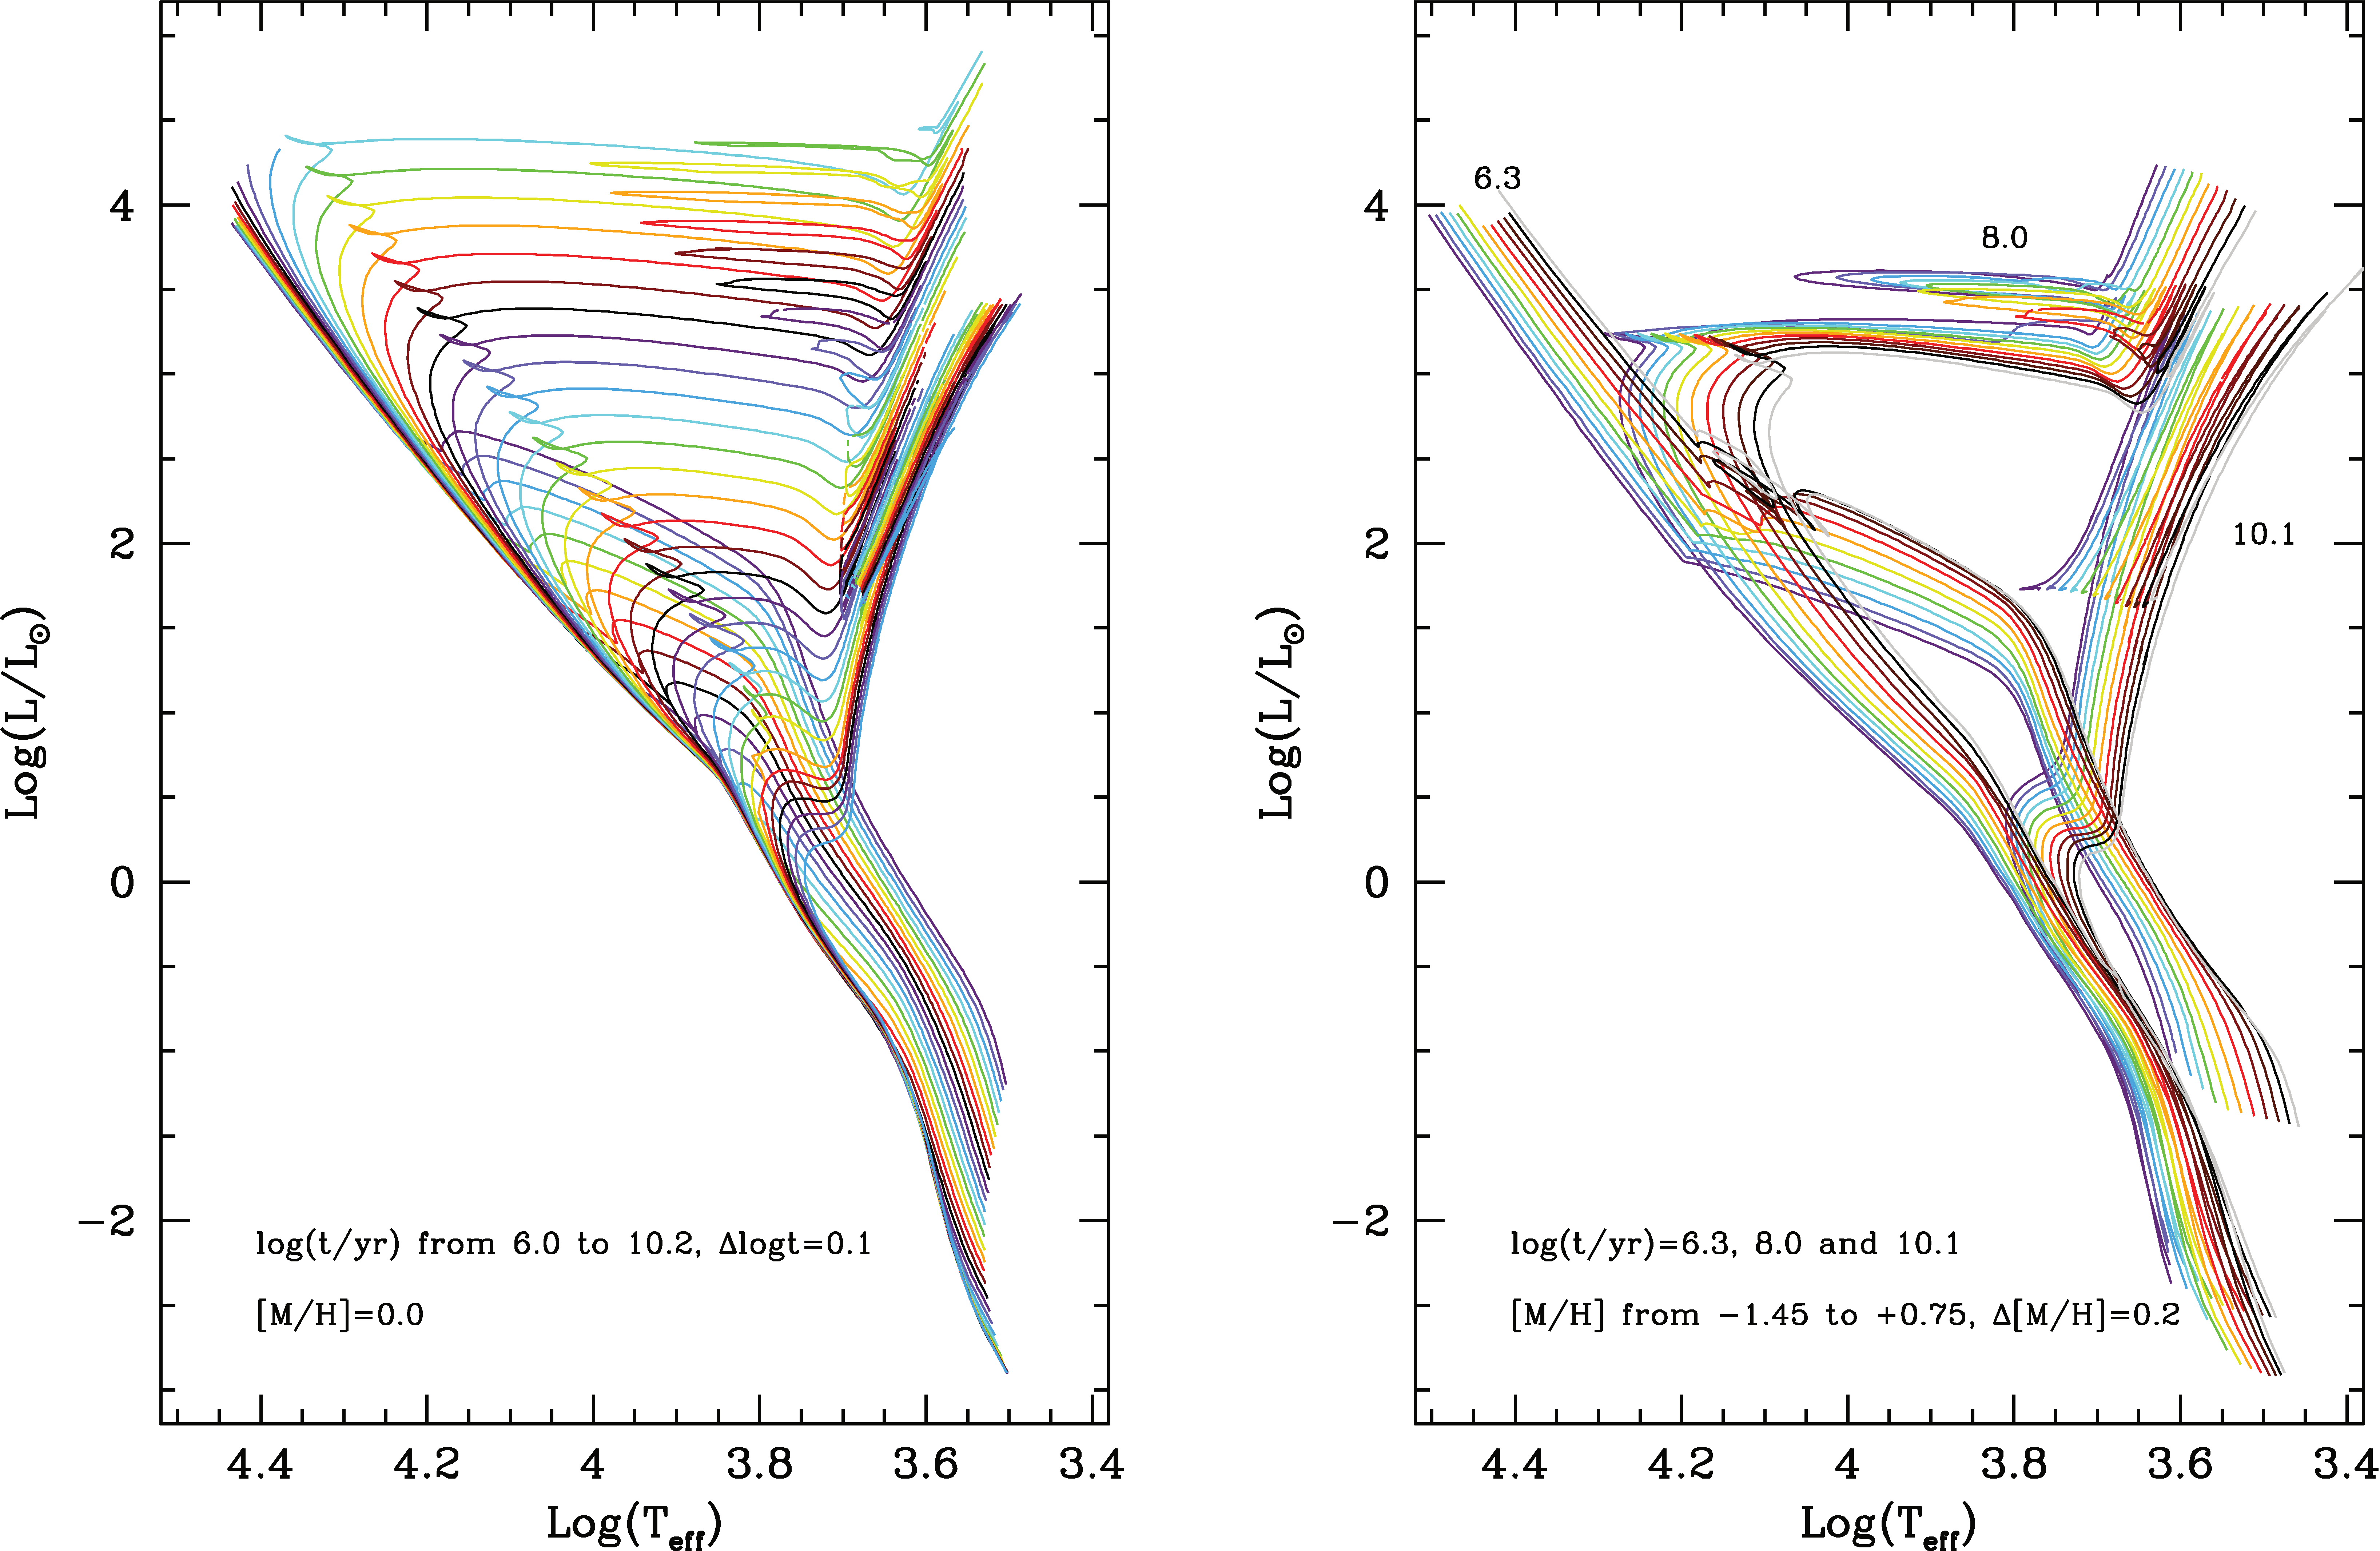
\includegraphics[width=0.9\textwidth]{../figures/theoretical_isochrones_in_hr_diagrams.pdf}
  \caption{Examples of theoretical isochrones in the H-R diagram taken from \protect\citeA[p.~16]{bressan2012parsec}}
  \label{fig:examples_of_isochrones}
\end{figure}

Since these stars were born close in time, they should have a sharp, well-defined profile with little scattering through the main sequence in the H-R diagram.
Examples for this kind of diagrams are presented in Figure \ref{fig:examples_of_hr_diagrams}.

\begin{figure}[htbp]
  \centering
  \begin{subfigure}{0.9\textwidth}
    \centering
    \begin{subfigure}[t]{0.45\textwidth}
      \centering
      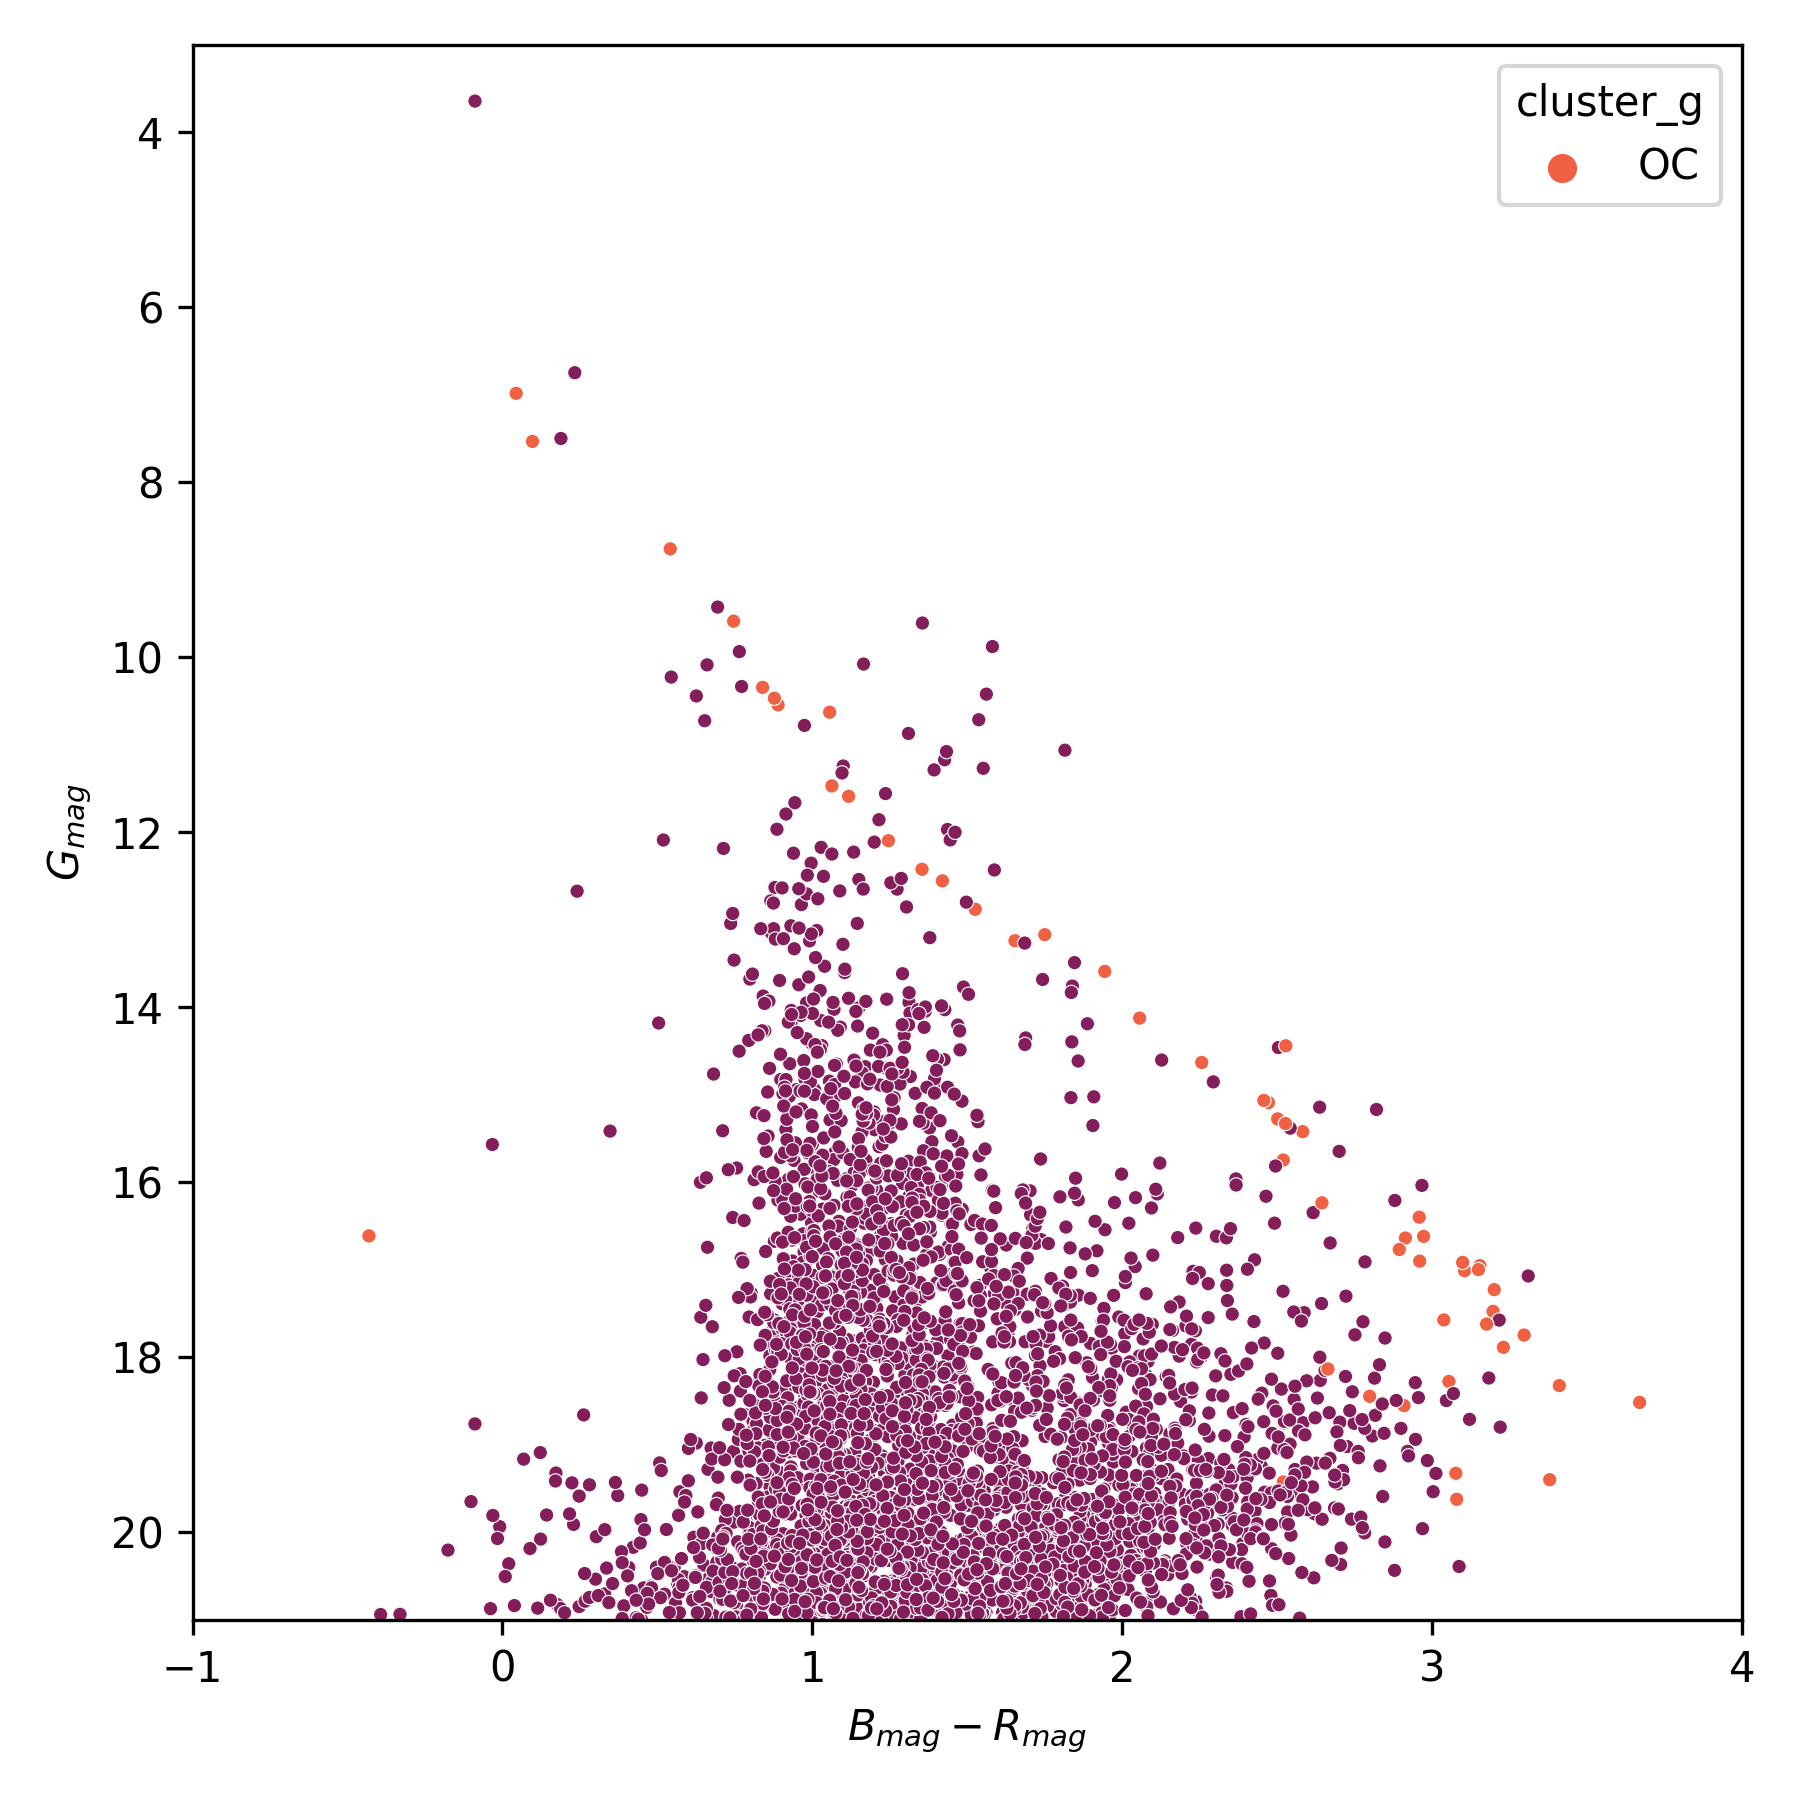
\includegraphics[width=\textwidth]{../figures/melotte_22/hr_diagram_melotte_22.png}
    \end{subfigure}
    \hfill
    \begin{subfigure}[t]{0.45\textwidth}
      \centering
      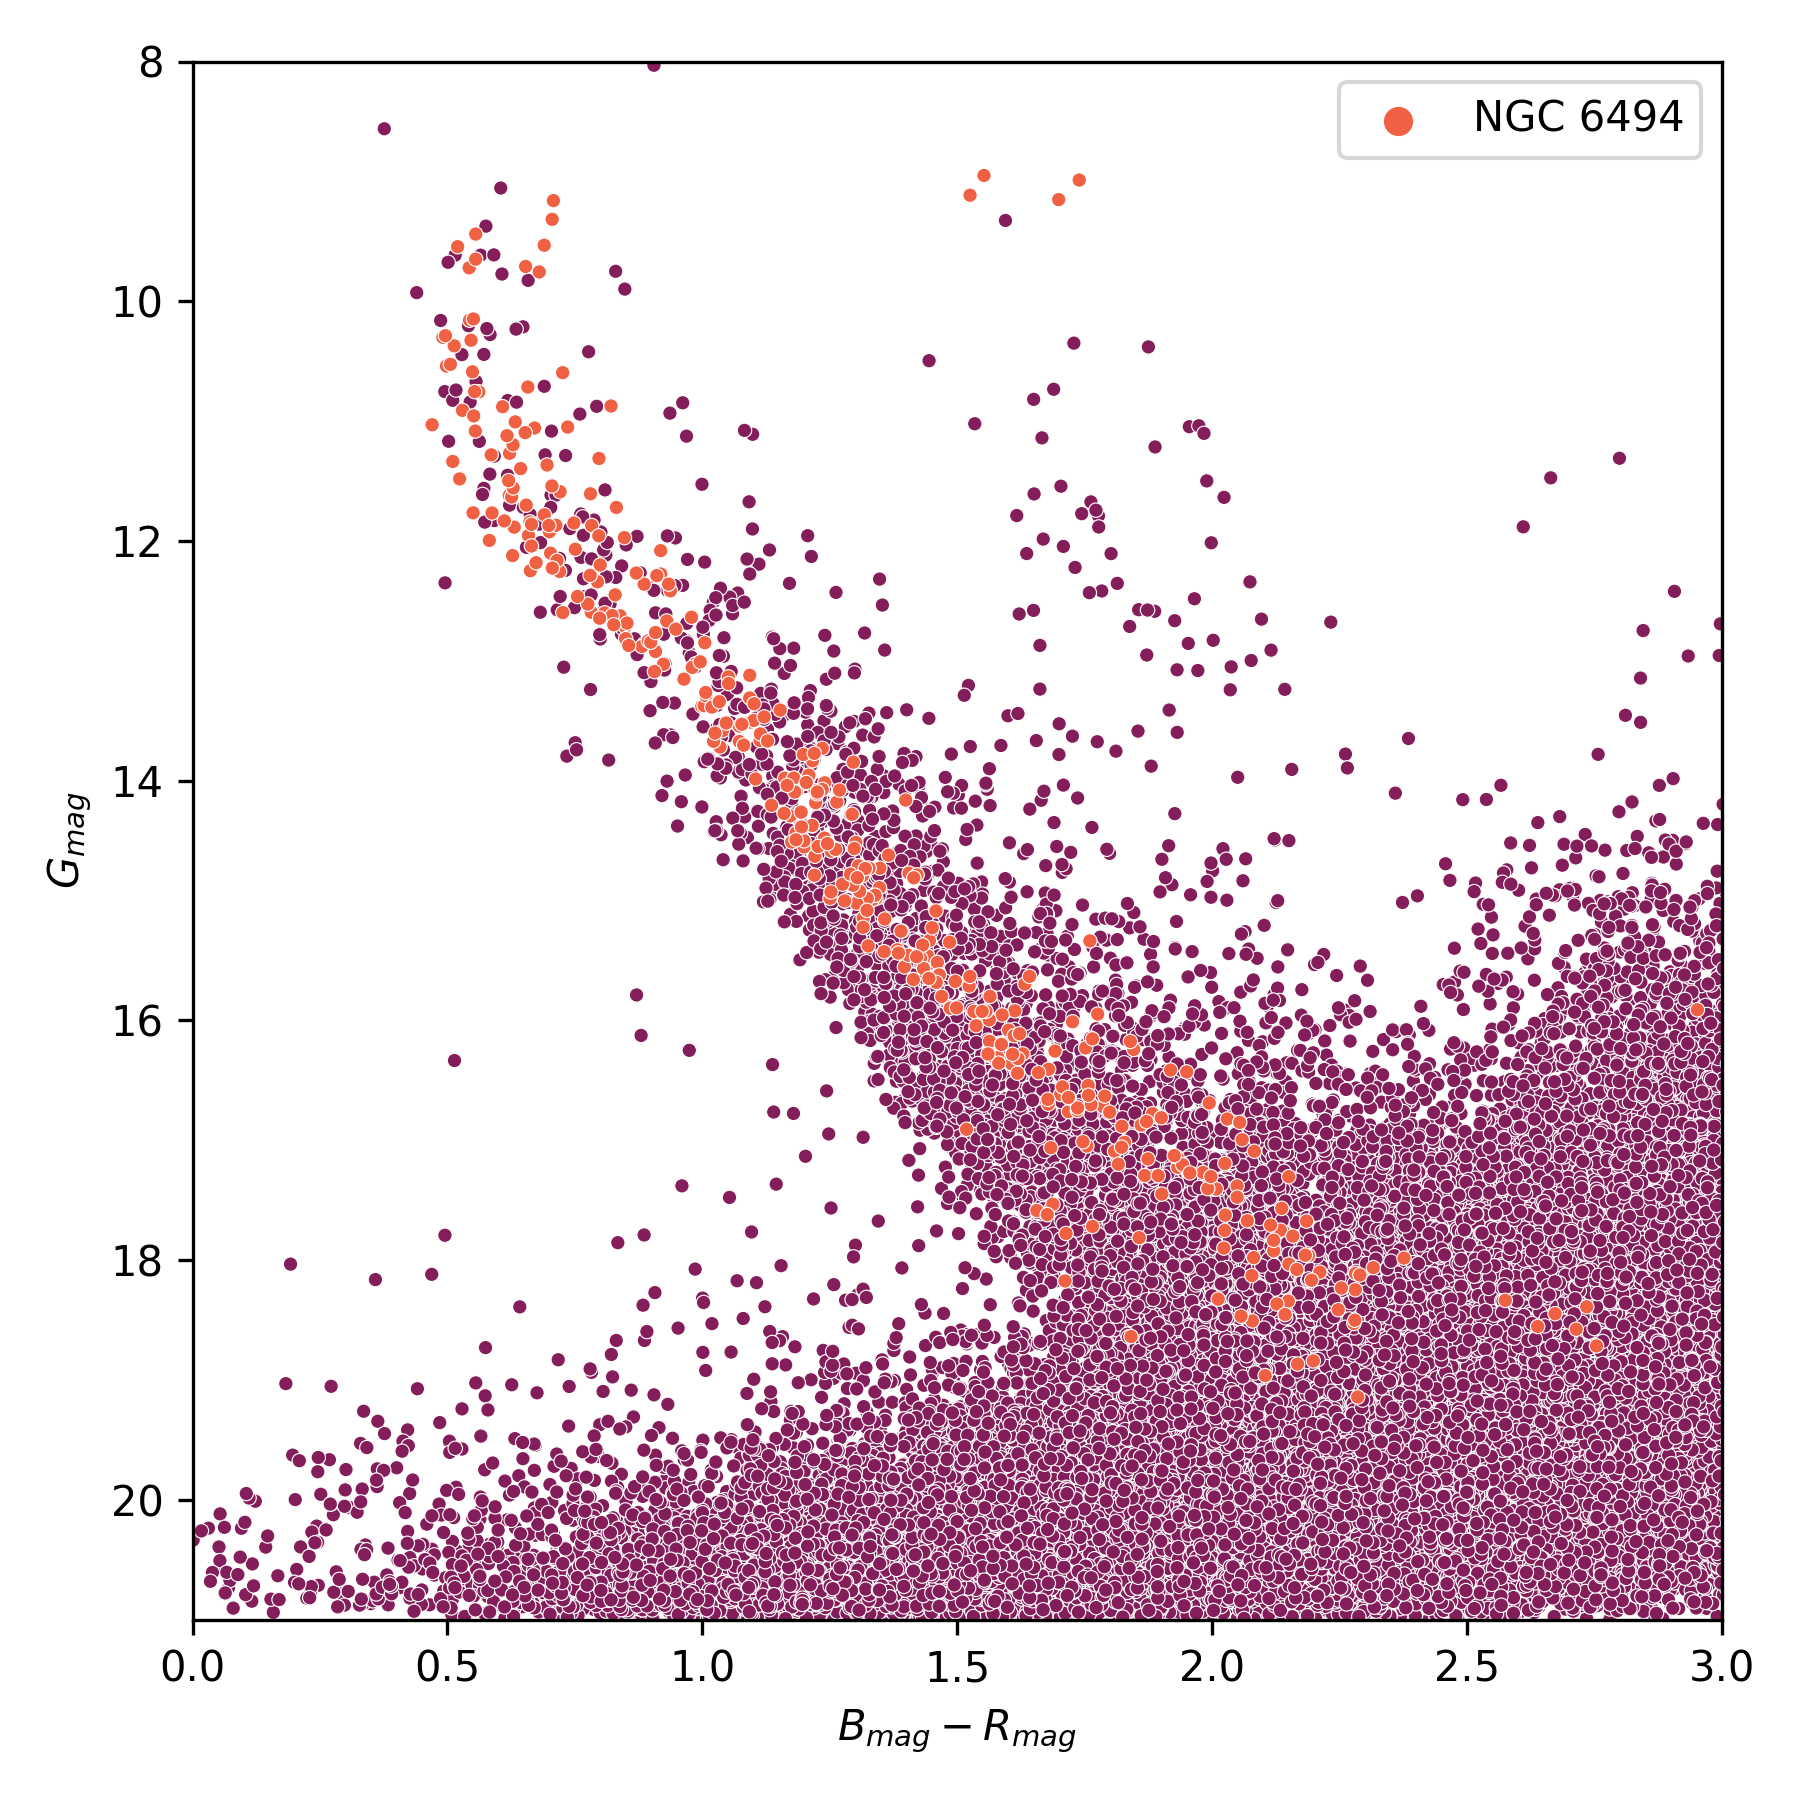
\includegraphics[width=\textwidth]{../figures/ngc_6494/hr_diagram_ngc_6494.png}
    \end{subfigure}
  \end{subfigure}
  \caption{Examples of typical profiles in H-R diagrams for members of open clusters. On the left Melotte 22, on the right NGC 6494.}
  \label{fig:examples_of_hr_diagrams}
\end{figure}

We will take advantage of these properties only to validate our characterization of OCs, but not to determine what stars belong to them. As we will explain later,
we will only use dynamic properties such as proper motions and parallax to characterize open clusters.

Although the members of a cluster appear in the observation visual field as an overdensity in positions, as shown in Figure \ref{fig:pos_ngc_2682}, these coordinates
are not useful to separate those stars that belong to the cluster from the other which do not. However, if we look for overdensities in the proper motions configuration space,
it is possible, at least at first instance, to assume a possible membership delimitation. See Figure \ref{fig:pm_ngc_2682}.

\begin{figure}[htbp]
  \centering
  \begin{subfigure}{0.9\textwidth}
    \centering
    \begin{subfigure}[t]{0.45\textwidth}
      \centering
      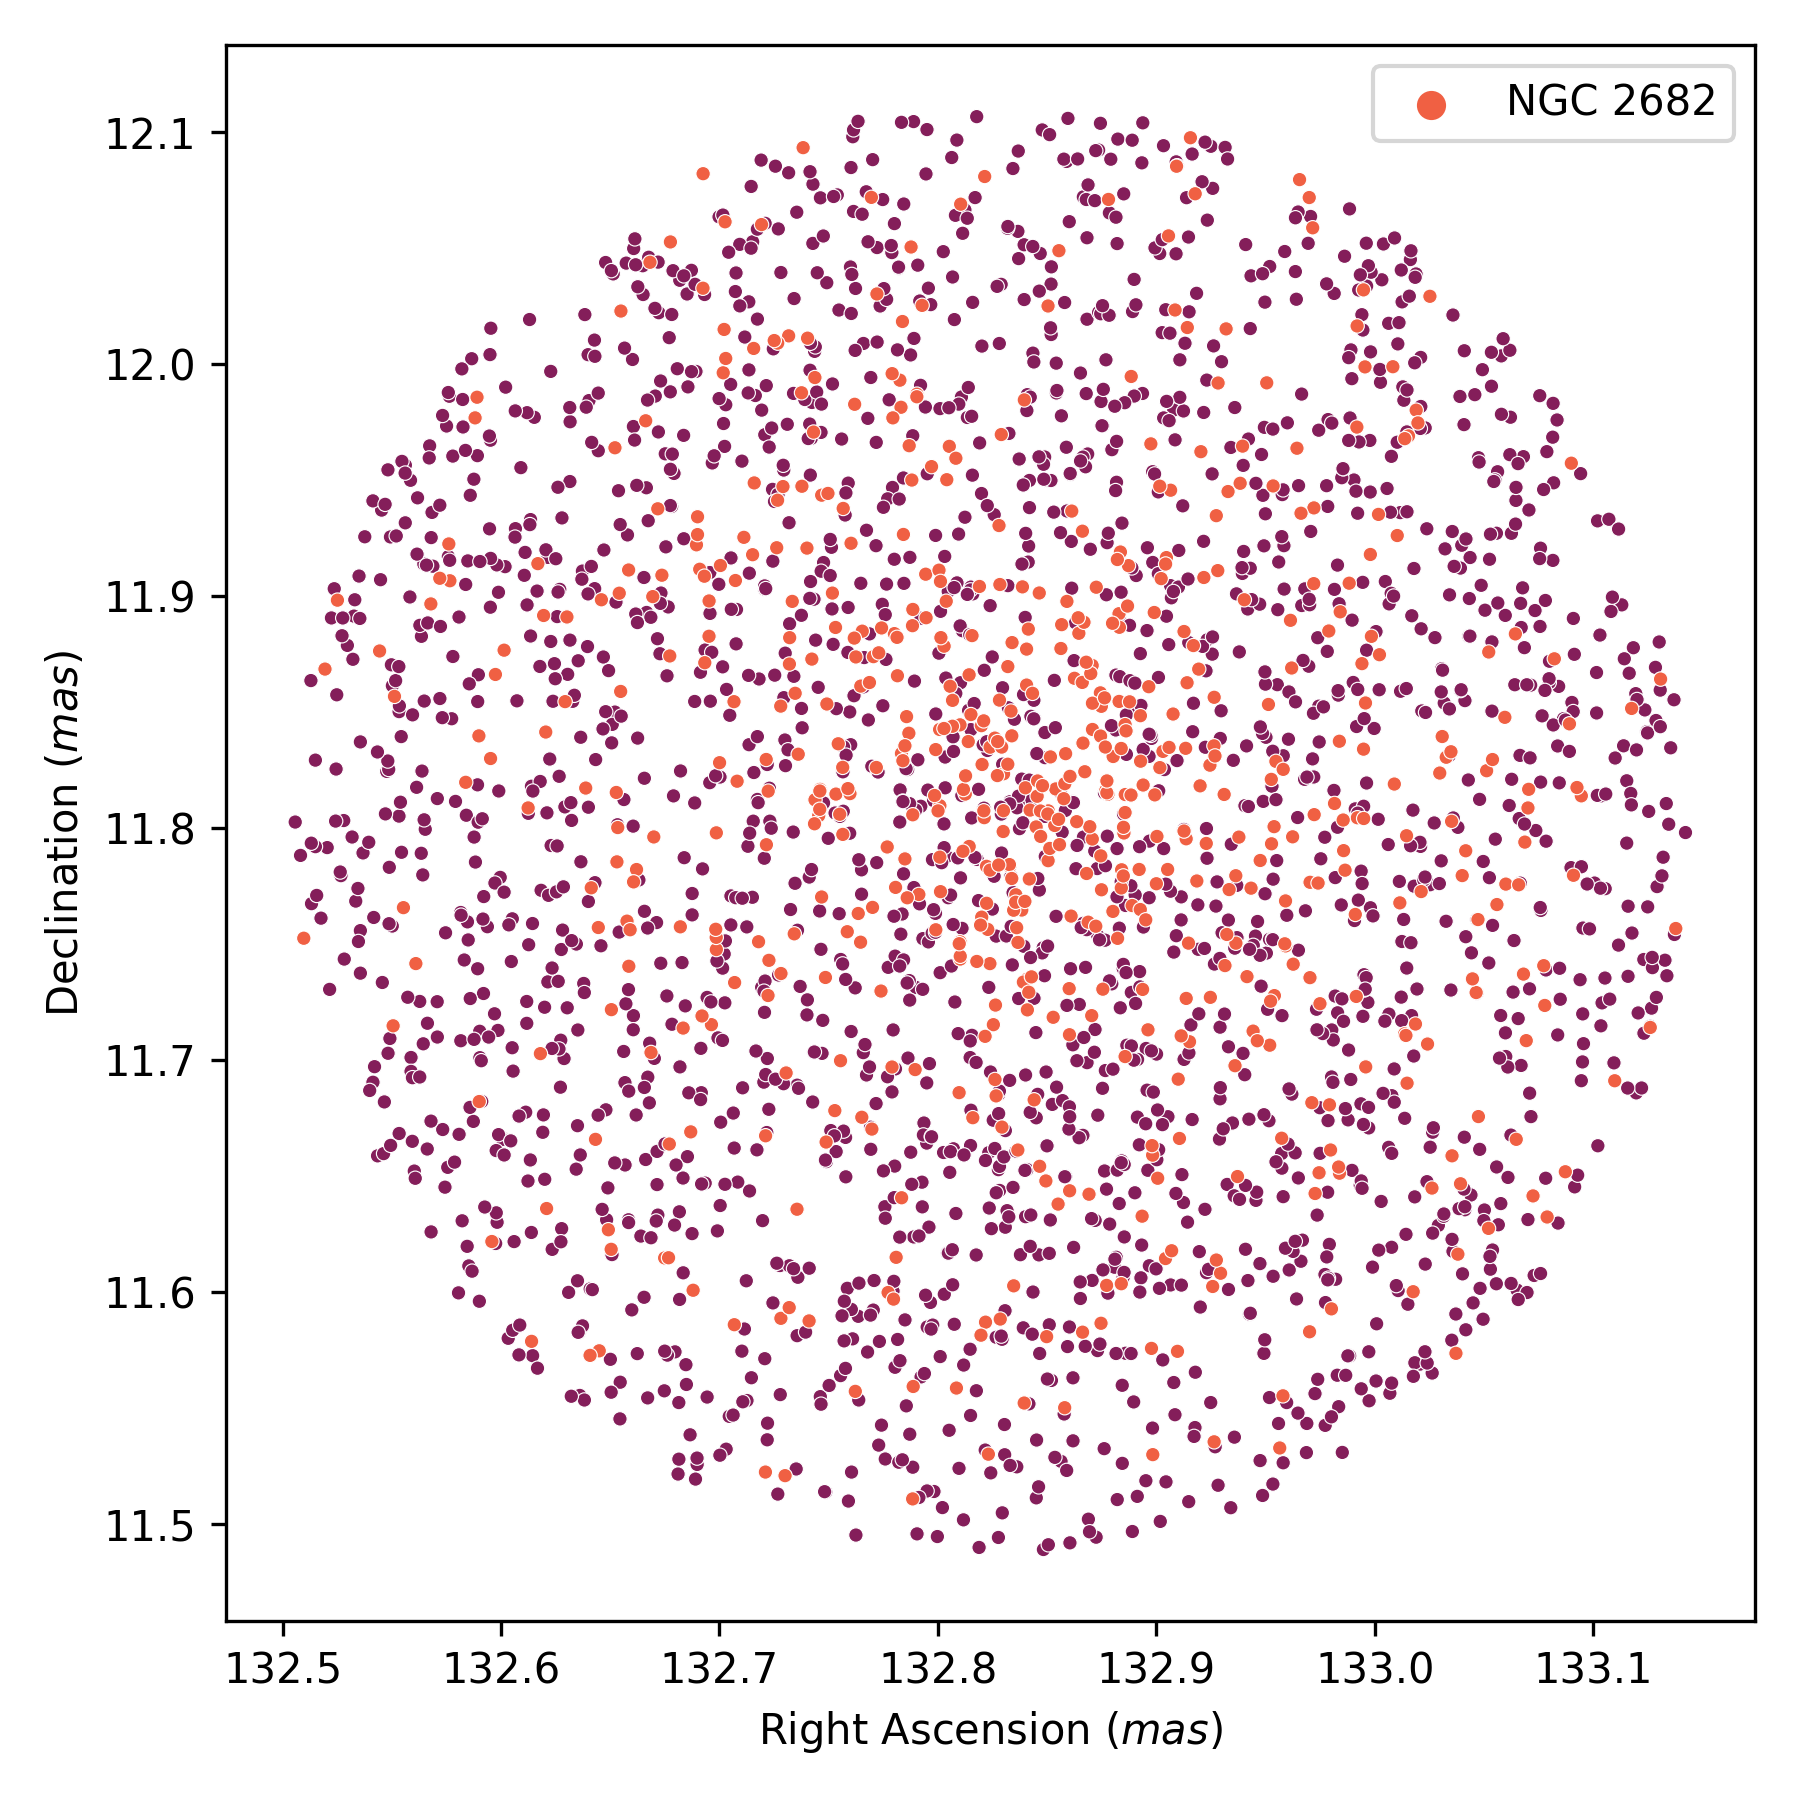
\includegraphics[width=\textwidth]{../figures/ngc_2682/pos_ngc_2682.png}
      \caption{Positions map}
      \label{fig:pos_ngc_2682}
    \end{subfigure}
    \hfill
    \begin{subfigure}[t]{0.45\textwidth}
      \centering
      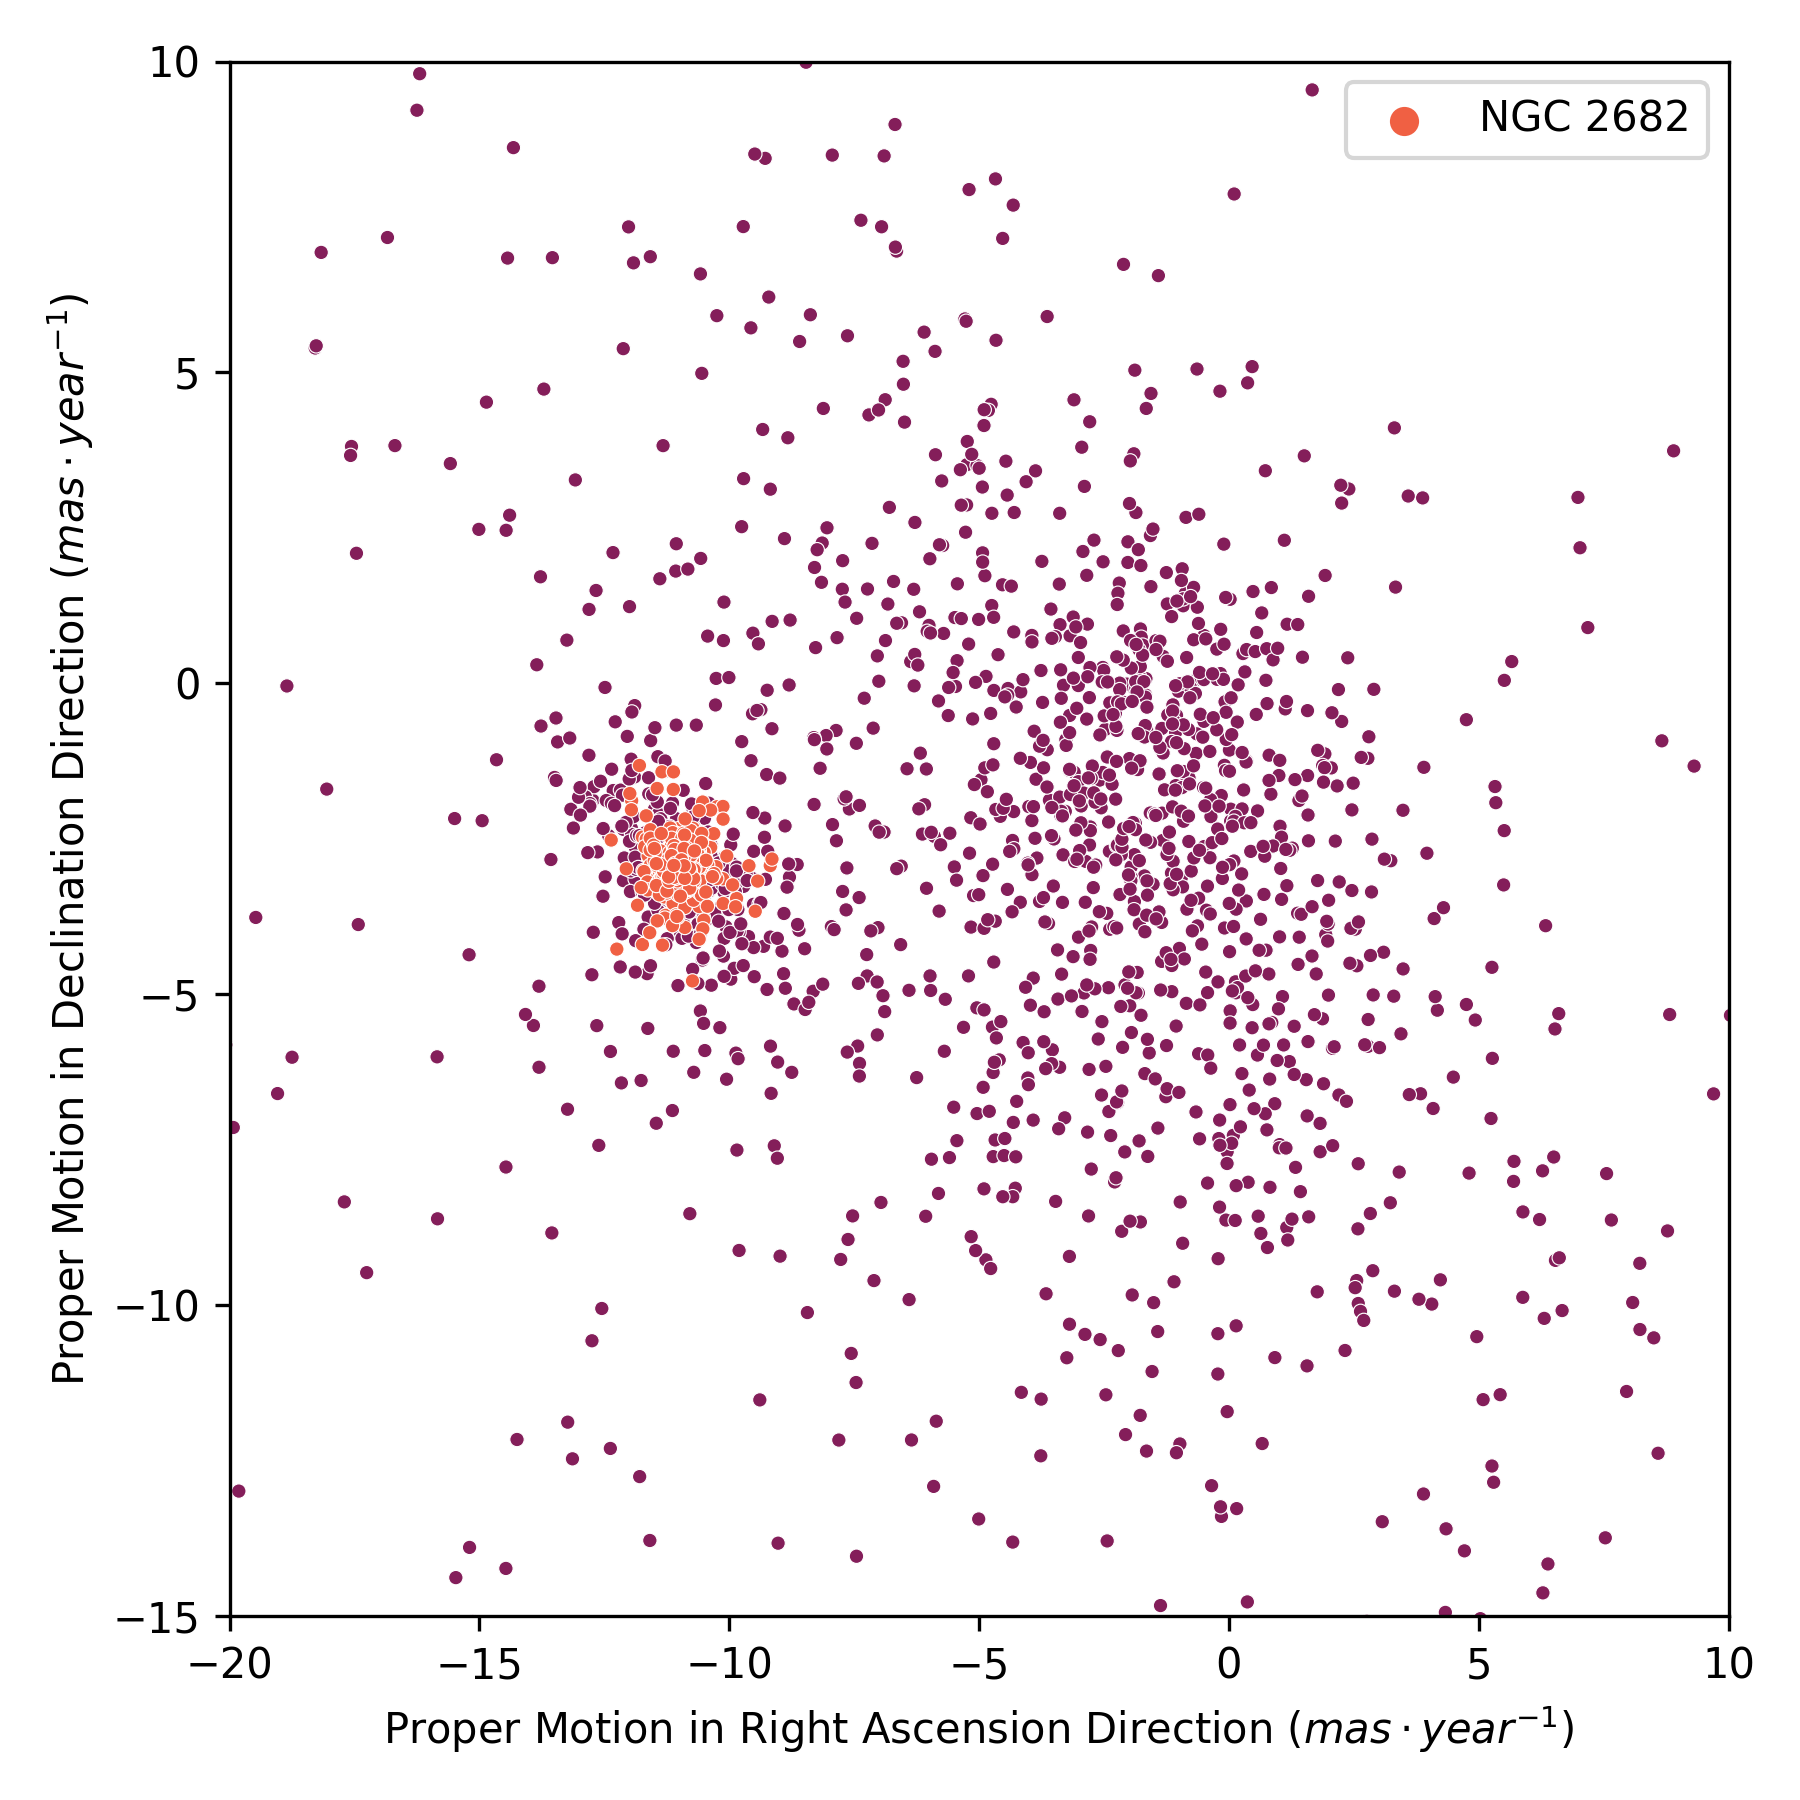
\includegraphics[width=\textwidth]{../figures/ngc_2682/pm_ngc_2682.png}
      \caption{Proper motions}
      \label{fig:pm_ngc_2682}
    \end{subfigure}
  \end{subfigure}
  \caption{NGC 2682 configuration spaces.}
\end{figure}

Overdensities in proper motion are not always so evident. Additionally, we will consider the parallax distribution to improve our cluster characterization.

\begin{figure}[htbp]
  \centering
  \begin{subfigure}{0.9\textwidth}
    \centering
    \begin{subfigure}[t]{0.45\textwidth}
      \centering
      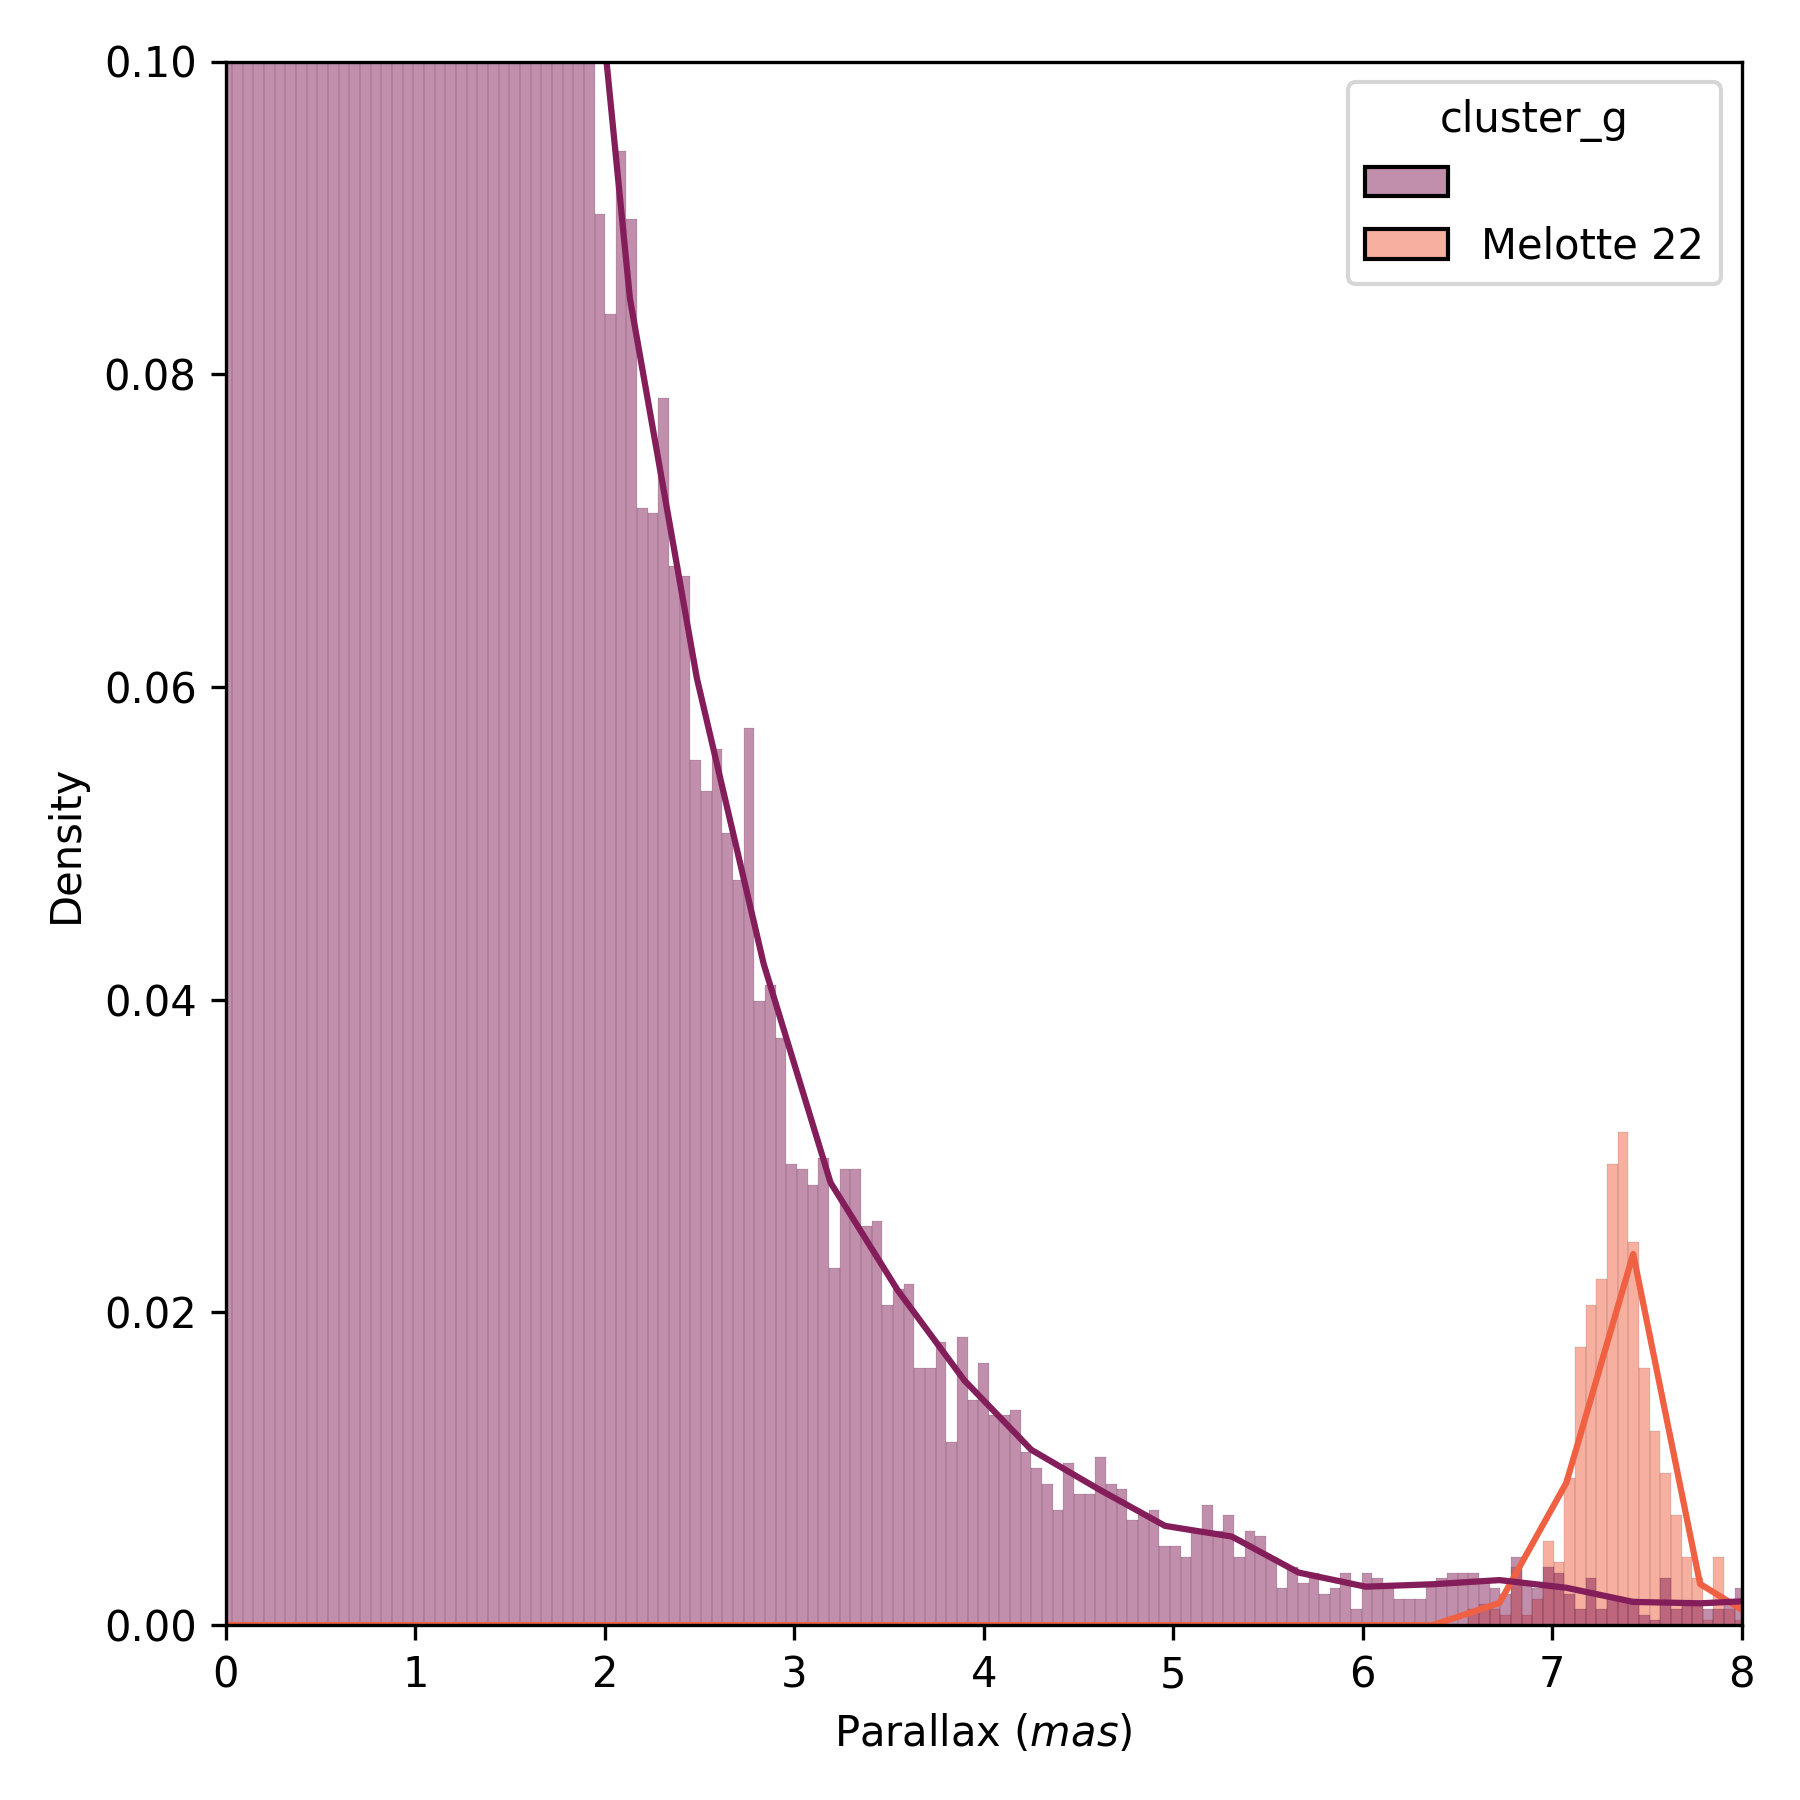
\includegraphics[width=\textwidth]{../figures/melotte_22/parallax_zoom_melotte_22.png}
      \caption{Melotte 22 Parallax}
      \label{fig:melotte_22_parallax_zoom}
    \end{subfigure}
    \hfill
    \begin{subfigure}[t]{0.45\textwidth}
      \centering
      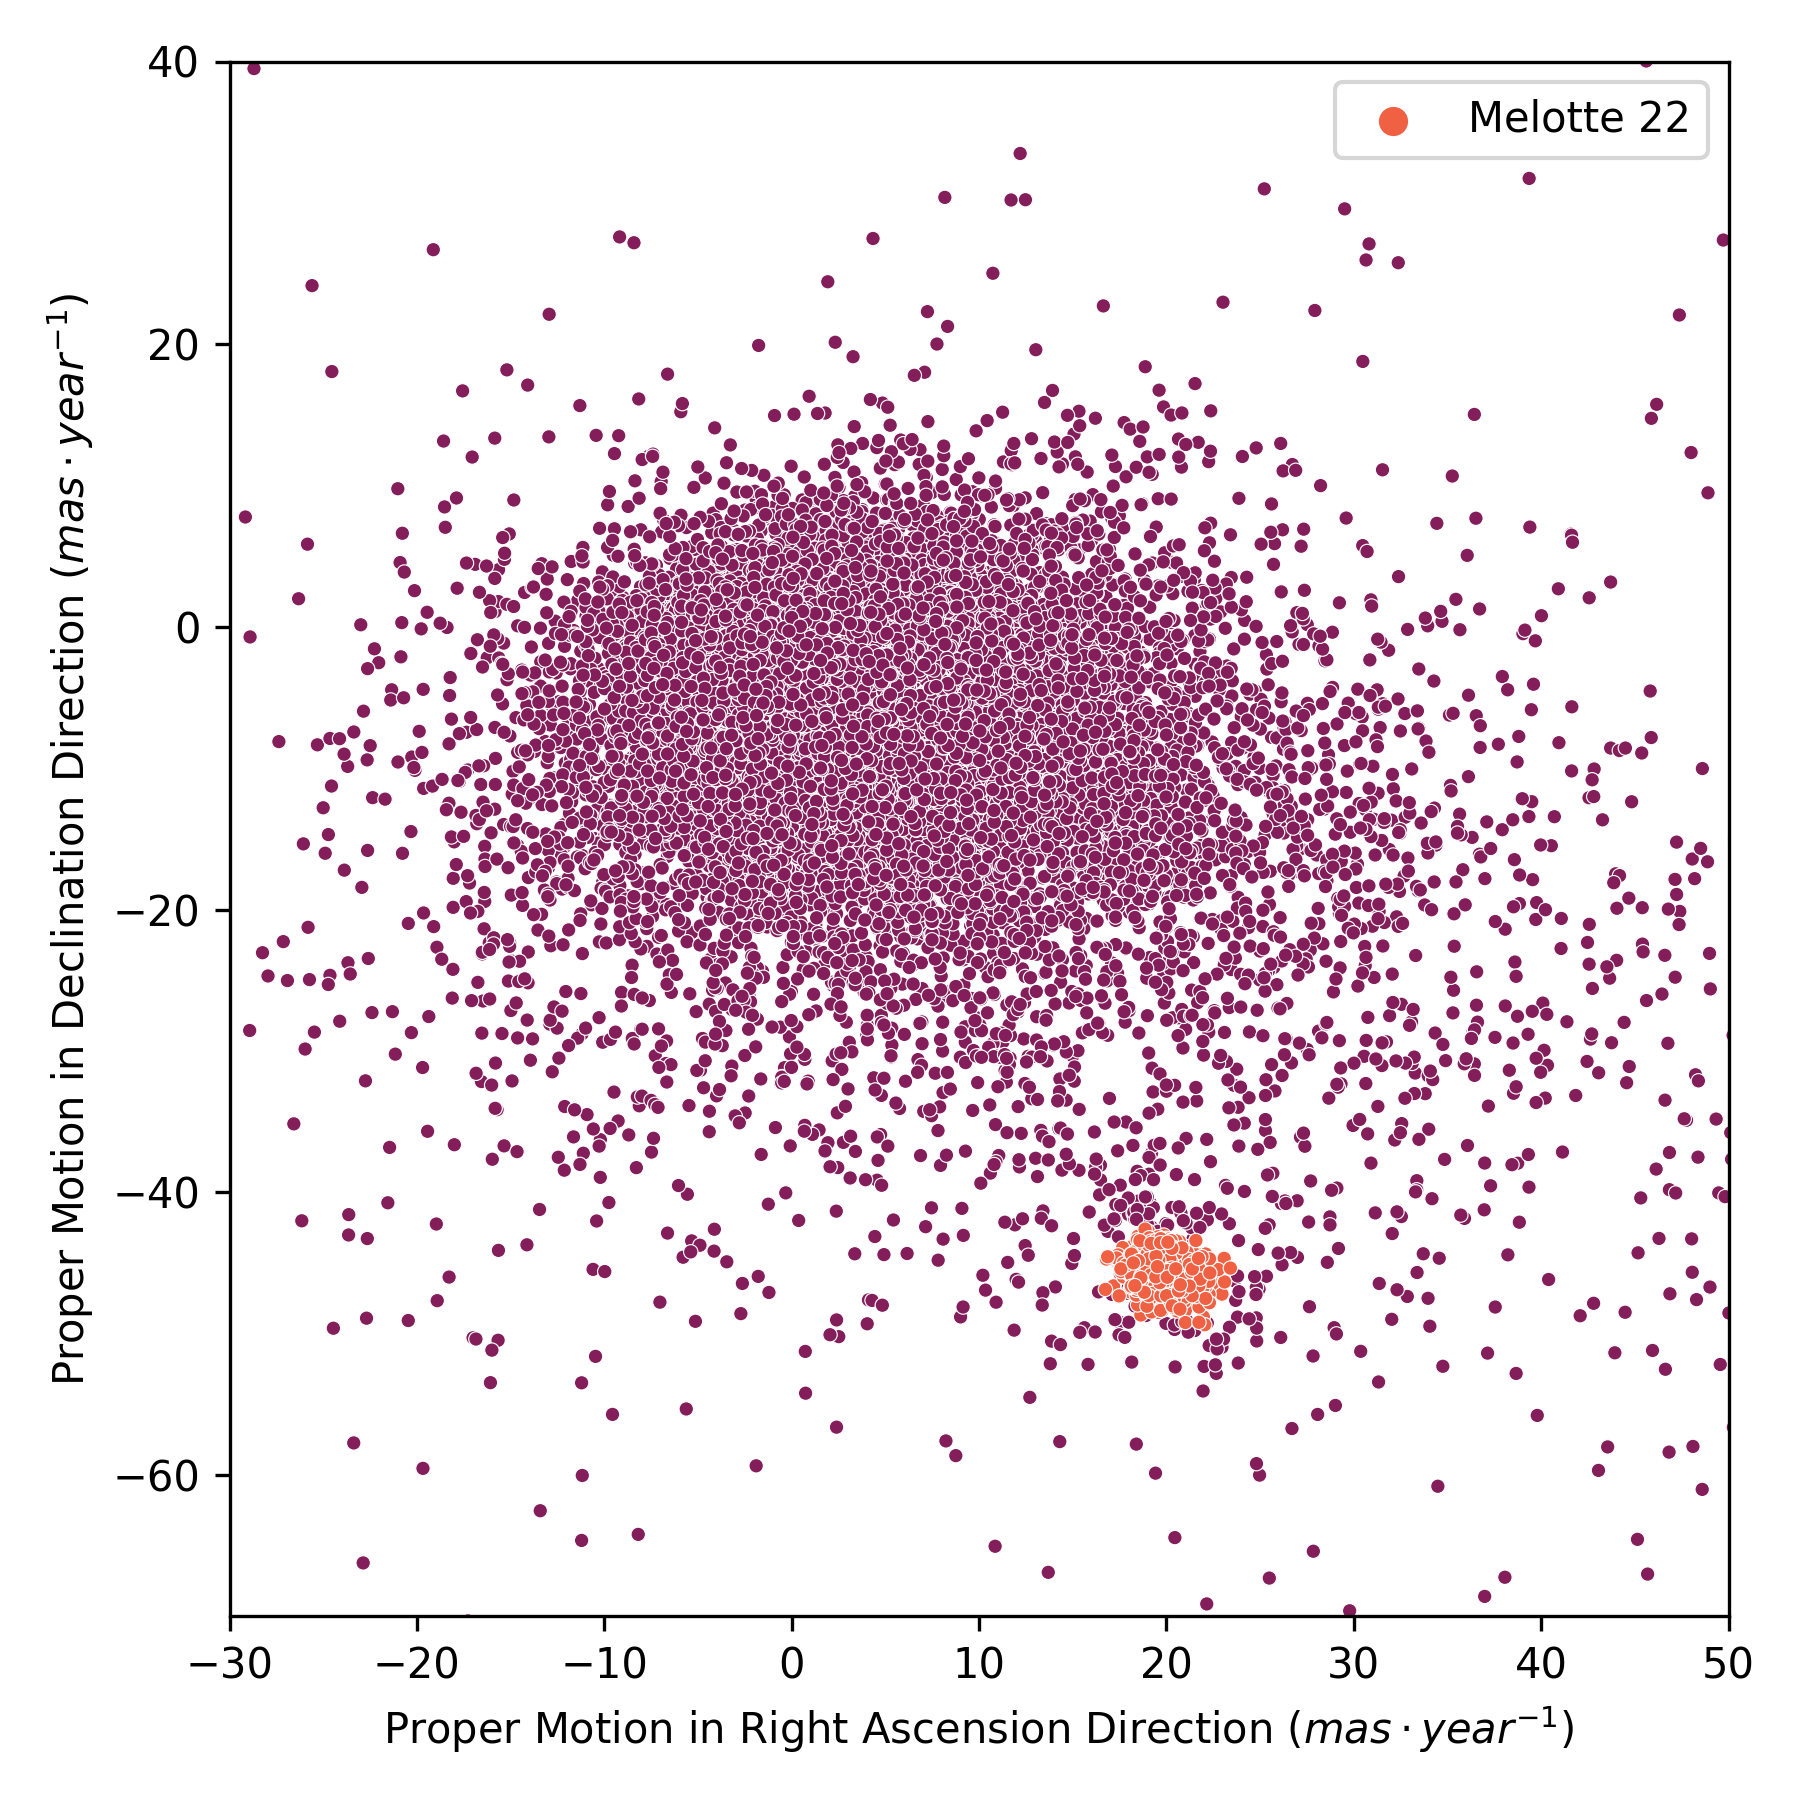
\includegraphics[width=\textwidth]{../figures/melotte_22/pm_melotte_22.png}
      \caption{Melotte 22 Proper motion}
    \end{subfigure}
  \end{subfigure}
  \caption{Melotte 22 Parallax histogram, clearly differentiated around the value $\approx 7.3mas$ and the corresponding diagram from the photometric magnitudes.}
  \label{fig:melotte_22_pm_parallax}
\end{figure}

In many other cases things are not so simple, and the characterization process can turn very difficult and tedious using tools such as the available ones at
the Virtual Observatory (VO), and frequently it requires parametrizations based on prior knowledge about the studied region. The aim of this work is to test
an unsupervised and non-parametrized model based on Machine Learning (ML) tools.

\chapter{Aims}

\section{General}

The main aim of this thesis is to \emph{build an unsupervised clustering model for open cluster characterization}.

We want this model to be \emph{non-supervised non-parameterized} in order to fit a wide range of clusters without
the need of fine tunning hyperparameters regarding the topology or size of the studied clusters.

\section{Specific}

To achieve the general goal, we will follow the following milestones:

\begin{itemize}
  \item Gather information on the \emph{state of the art}.
  \item Research unsupervised clustering algorithms suitable for grouping stars previously recovered.
  \item Recover data from Gaia DR2 database. This data will be taken as source for the machine learning model to characterize open clusters
  by grouping stars into clusters.
  \item Select and implement unsupervised clustering algorithms from the previous study.
  \item Use those algorithms with different datasets to find OCs.
  \item Look for an independent method to characterize OCs in order to make comparisons.
  \item Validate found OCs with our custom model by making comparisons with the independent method.
\end{itemize}

\chapter{State of the Art}

% TODO: Hablar de la misión Gaia
% TODO: Hablar de KMedias y DEC
% TODO: Mencionar trabajos relacionados

An initial approach to find OC is the search of overdensities along the galactic disk. In general, this is the initial point,
but even it looks simple, it presents a fundamental problem. The near field around the OC is fulled by two differenciated
kind of stars populations: the ones which belong to the OC (from a tens or hundreds to a few thousand) and a background composed
by thousands or millions of stars which don't belong to the OC. Find out which stars belong to the first group is the problem
treated in this work. This selection is crucial to properly characterize the fundamental properties of the cluster
(dynamics, total mass, age, chemical composition, etc.).

Sometimes, this problem is easy to solve by looking into astrometric parameters, such as the analysis of proper motion of those
stars belonging to the overdensity field.

\begin{figure}[htbp]
  \centering
  \begin{subfigure}{0.9\textwidth}
    \centering
    \begin{subfigure}[t]{0.45\textwidth}
      \centering
      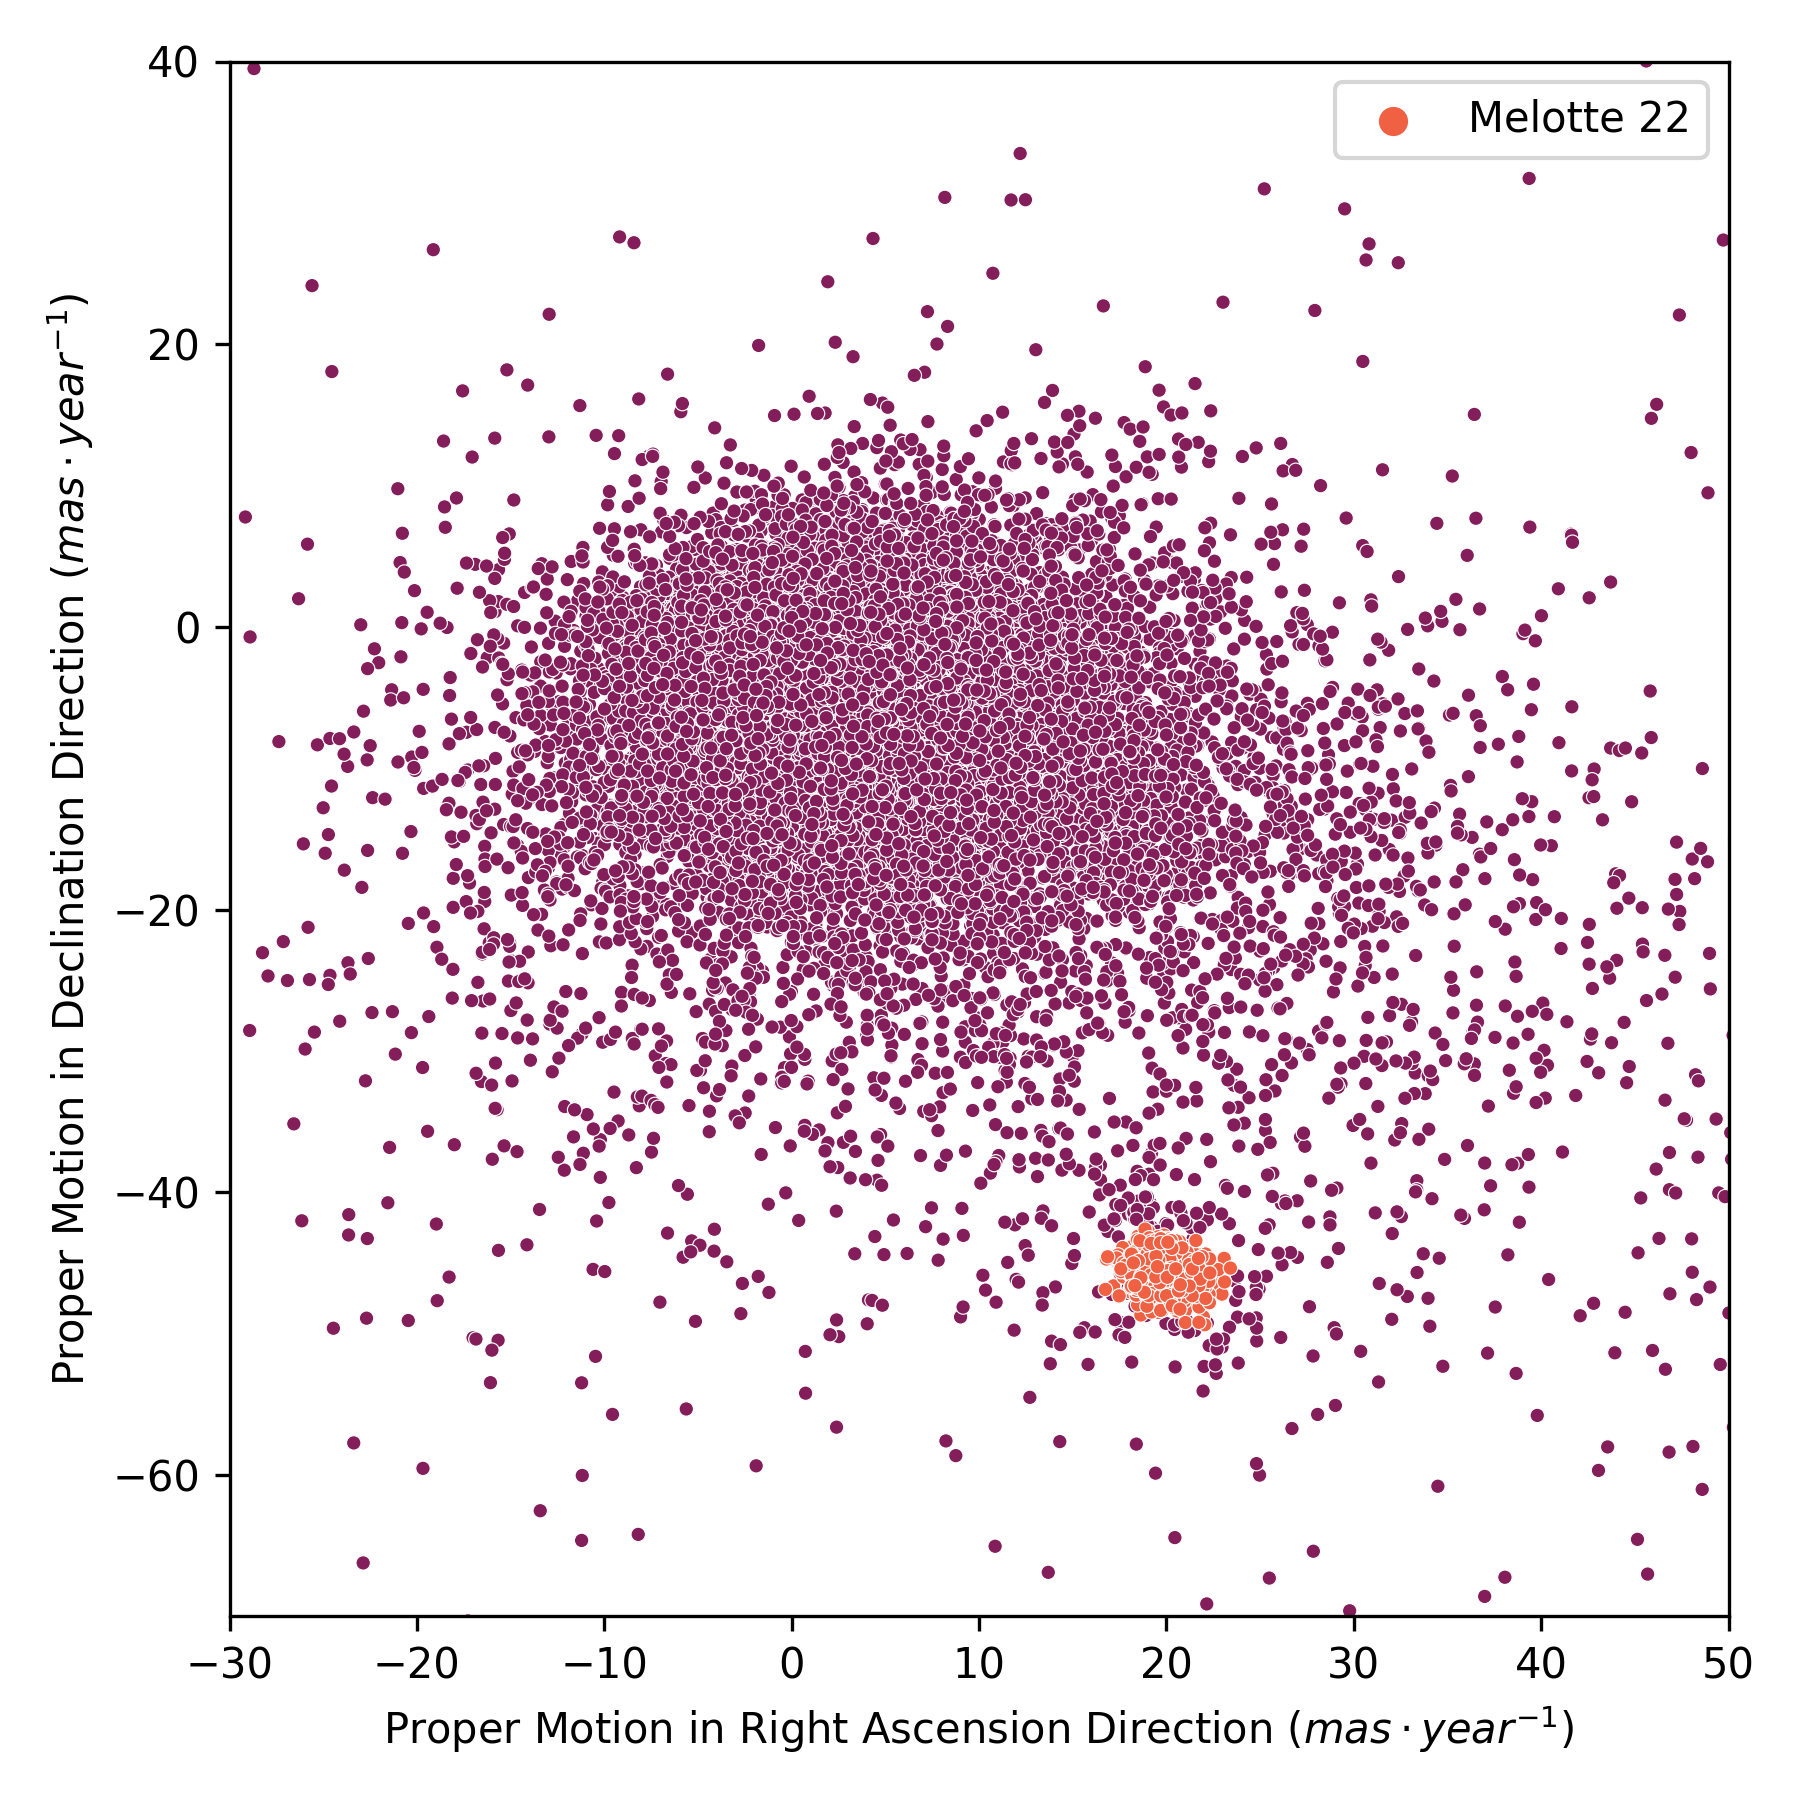
\includegraphics[width=\textwidth]{../figures/melotte_22/pm_melotte_22.png}
      \caption{Proper motions}
      \label{fig:pm_melotte_22}
    \end{subfigure}
    \hfill
    \begin{subfigure}[t]{0.45\textwidth}
      \centering
      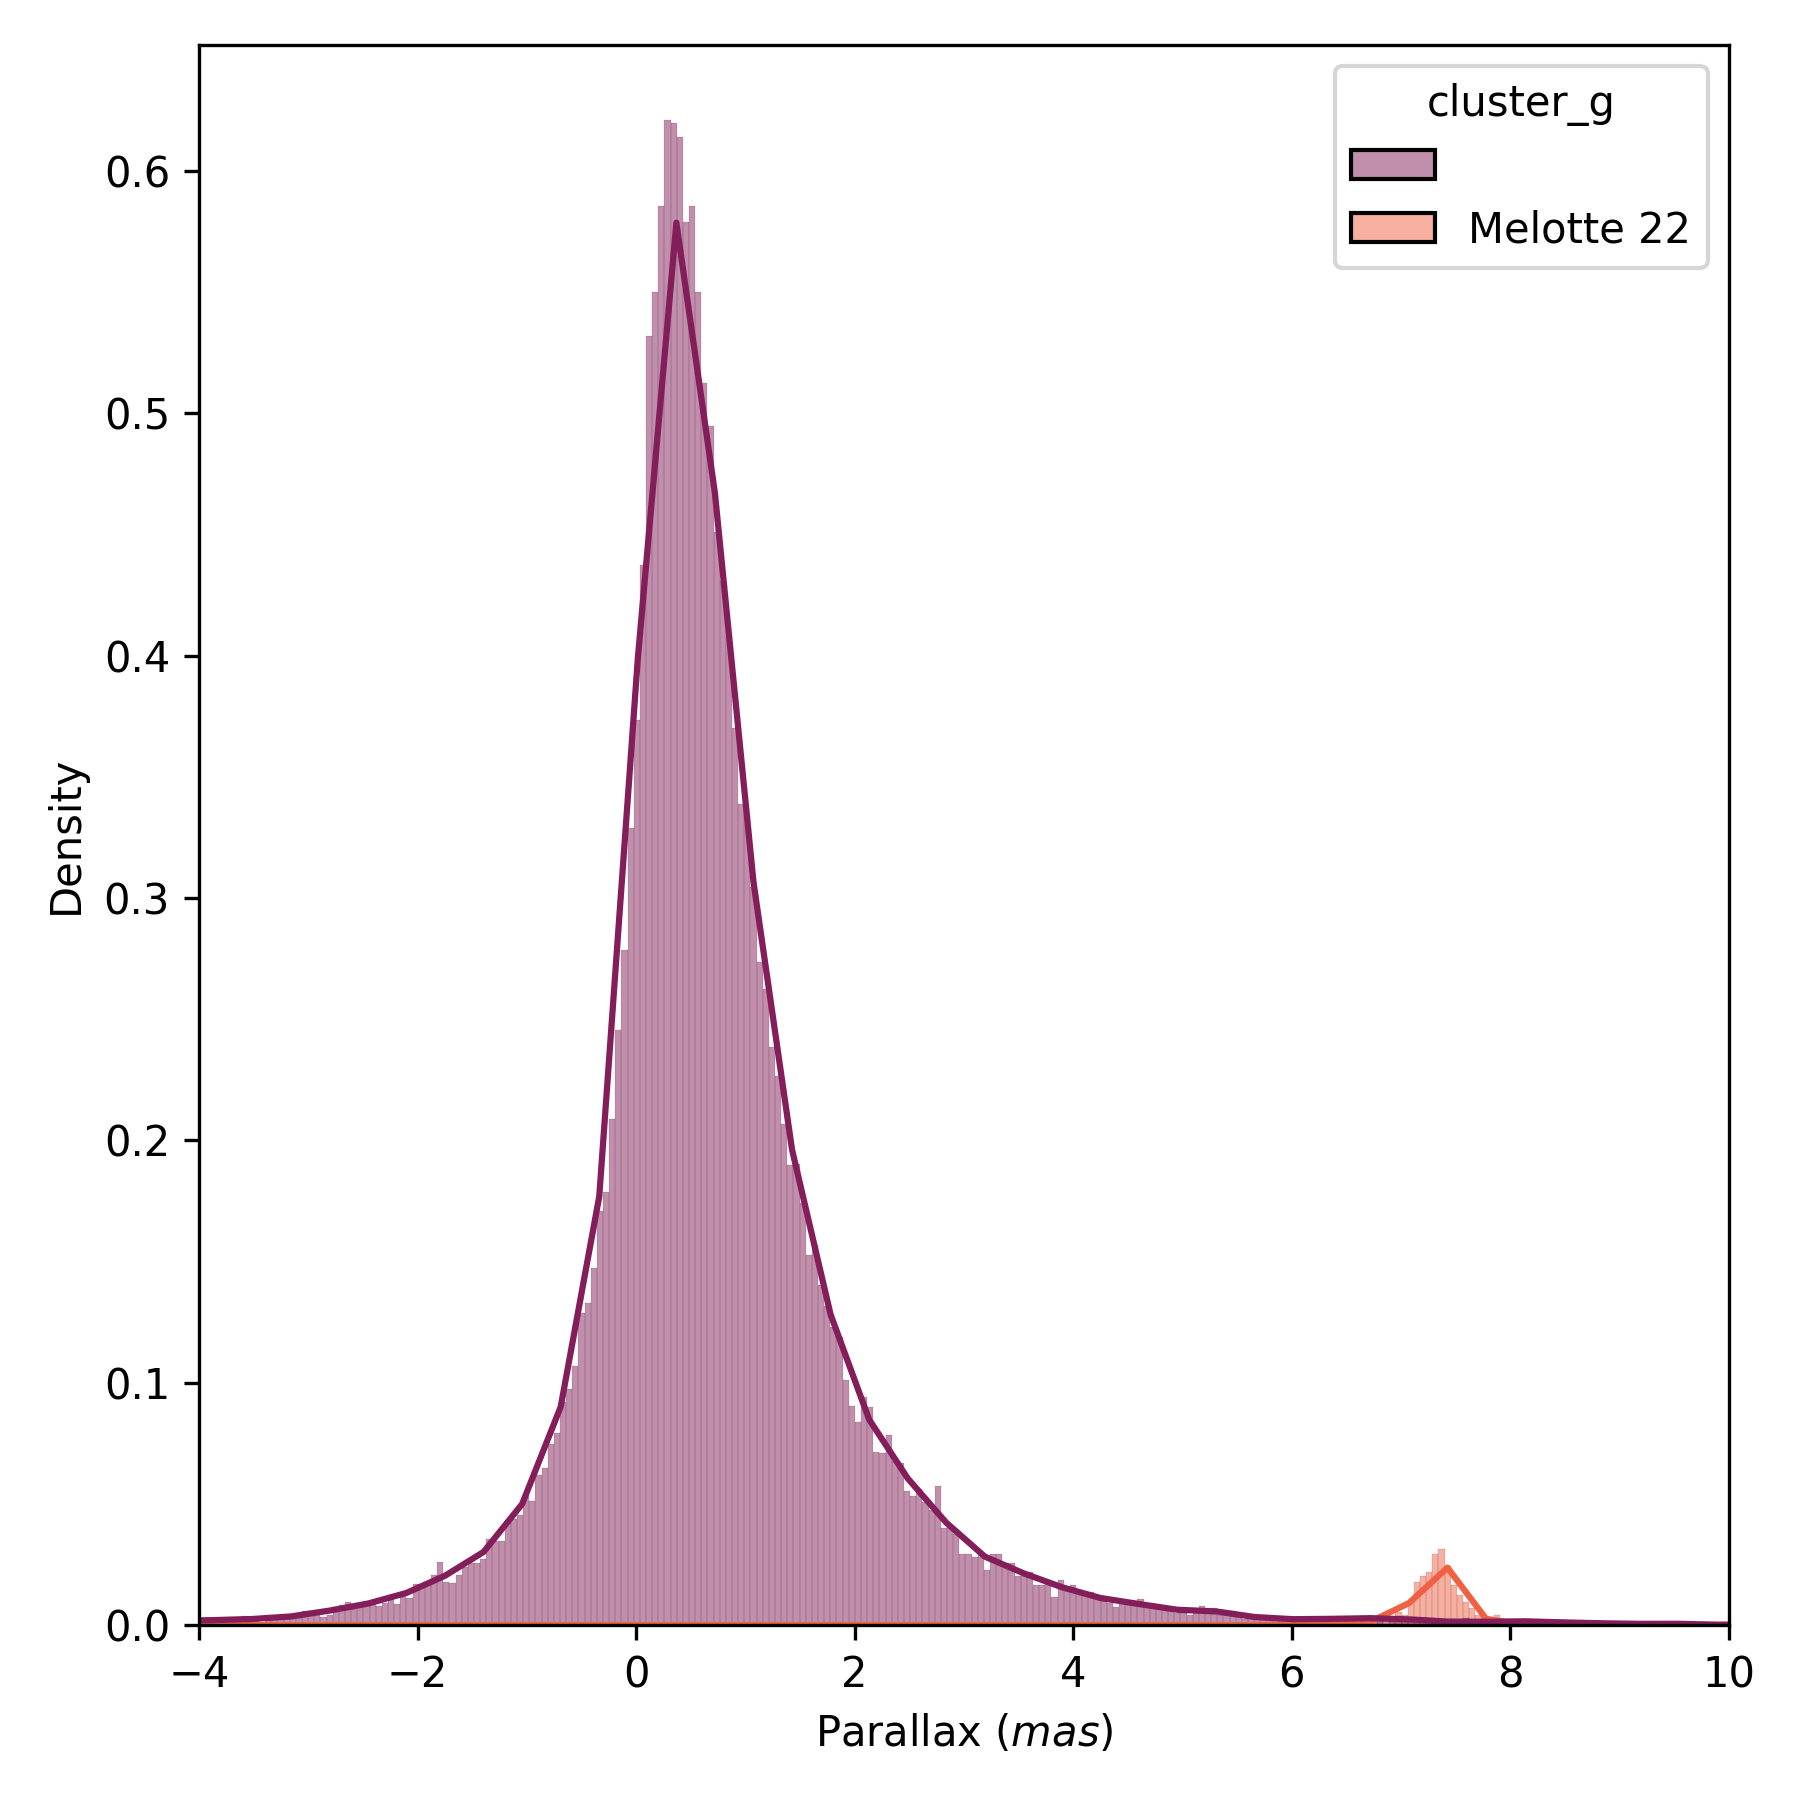
\includegraphics[width=\textwidth]{../figures/melotte_22/parallax_melotte_22.png}
      \caption{Parallax}
      \label{fig:pm_vec_melotte_22}
    \end{subfigure}
  \end{subfigure}
  \caption{Open Cluster Melotte 22 (Messier 45)}
\end{figure}

Figure \ref{fig:pm_melotte_22} shows the proper motion distribution in right ascension and declination.
It is easy to see that a subgroup can be located at [20, -45].
Figure \ref{fig:pm_vec_melotte_22} shows the parallax density and confirms an overdensity at $\approx 7.5 mas$ corresponding to Mellote 22 OC.

However, as shown in Figures \ref{fig:pm_ngc_6494} and \ref{fig:parallax_ngc_6494}, in general it is not as easy and
becomes necessary to consider other parameters such as distances, or even metallicity and age (derived from isochrone curves)
and requires photometric data from stars in the studied field
\footnote{All figures have been sampled in order to reduce the document size, but are still a faithful representation of the original data}.

\begin{figure}[htbp]
  \centering
  \begin{subfigure}{0.9\textwidth}
    \centering
    \begin{subfigure}[t]{0.45\textwidth}
      \centering
      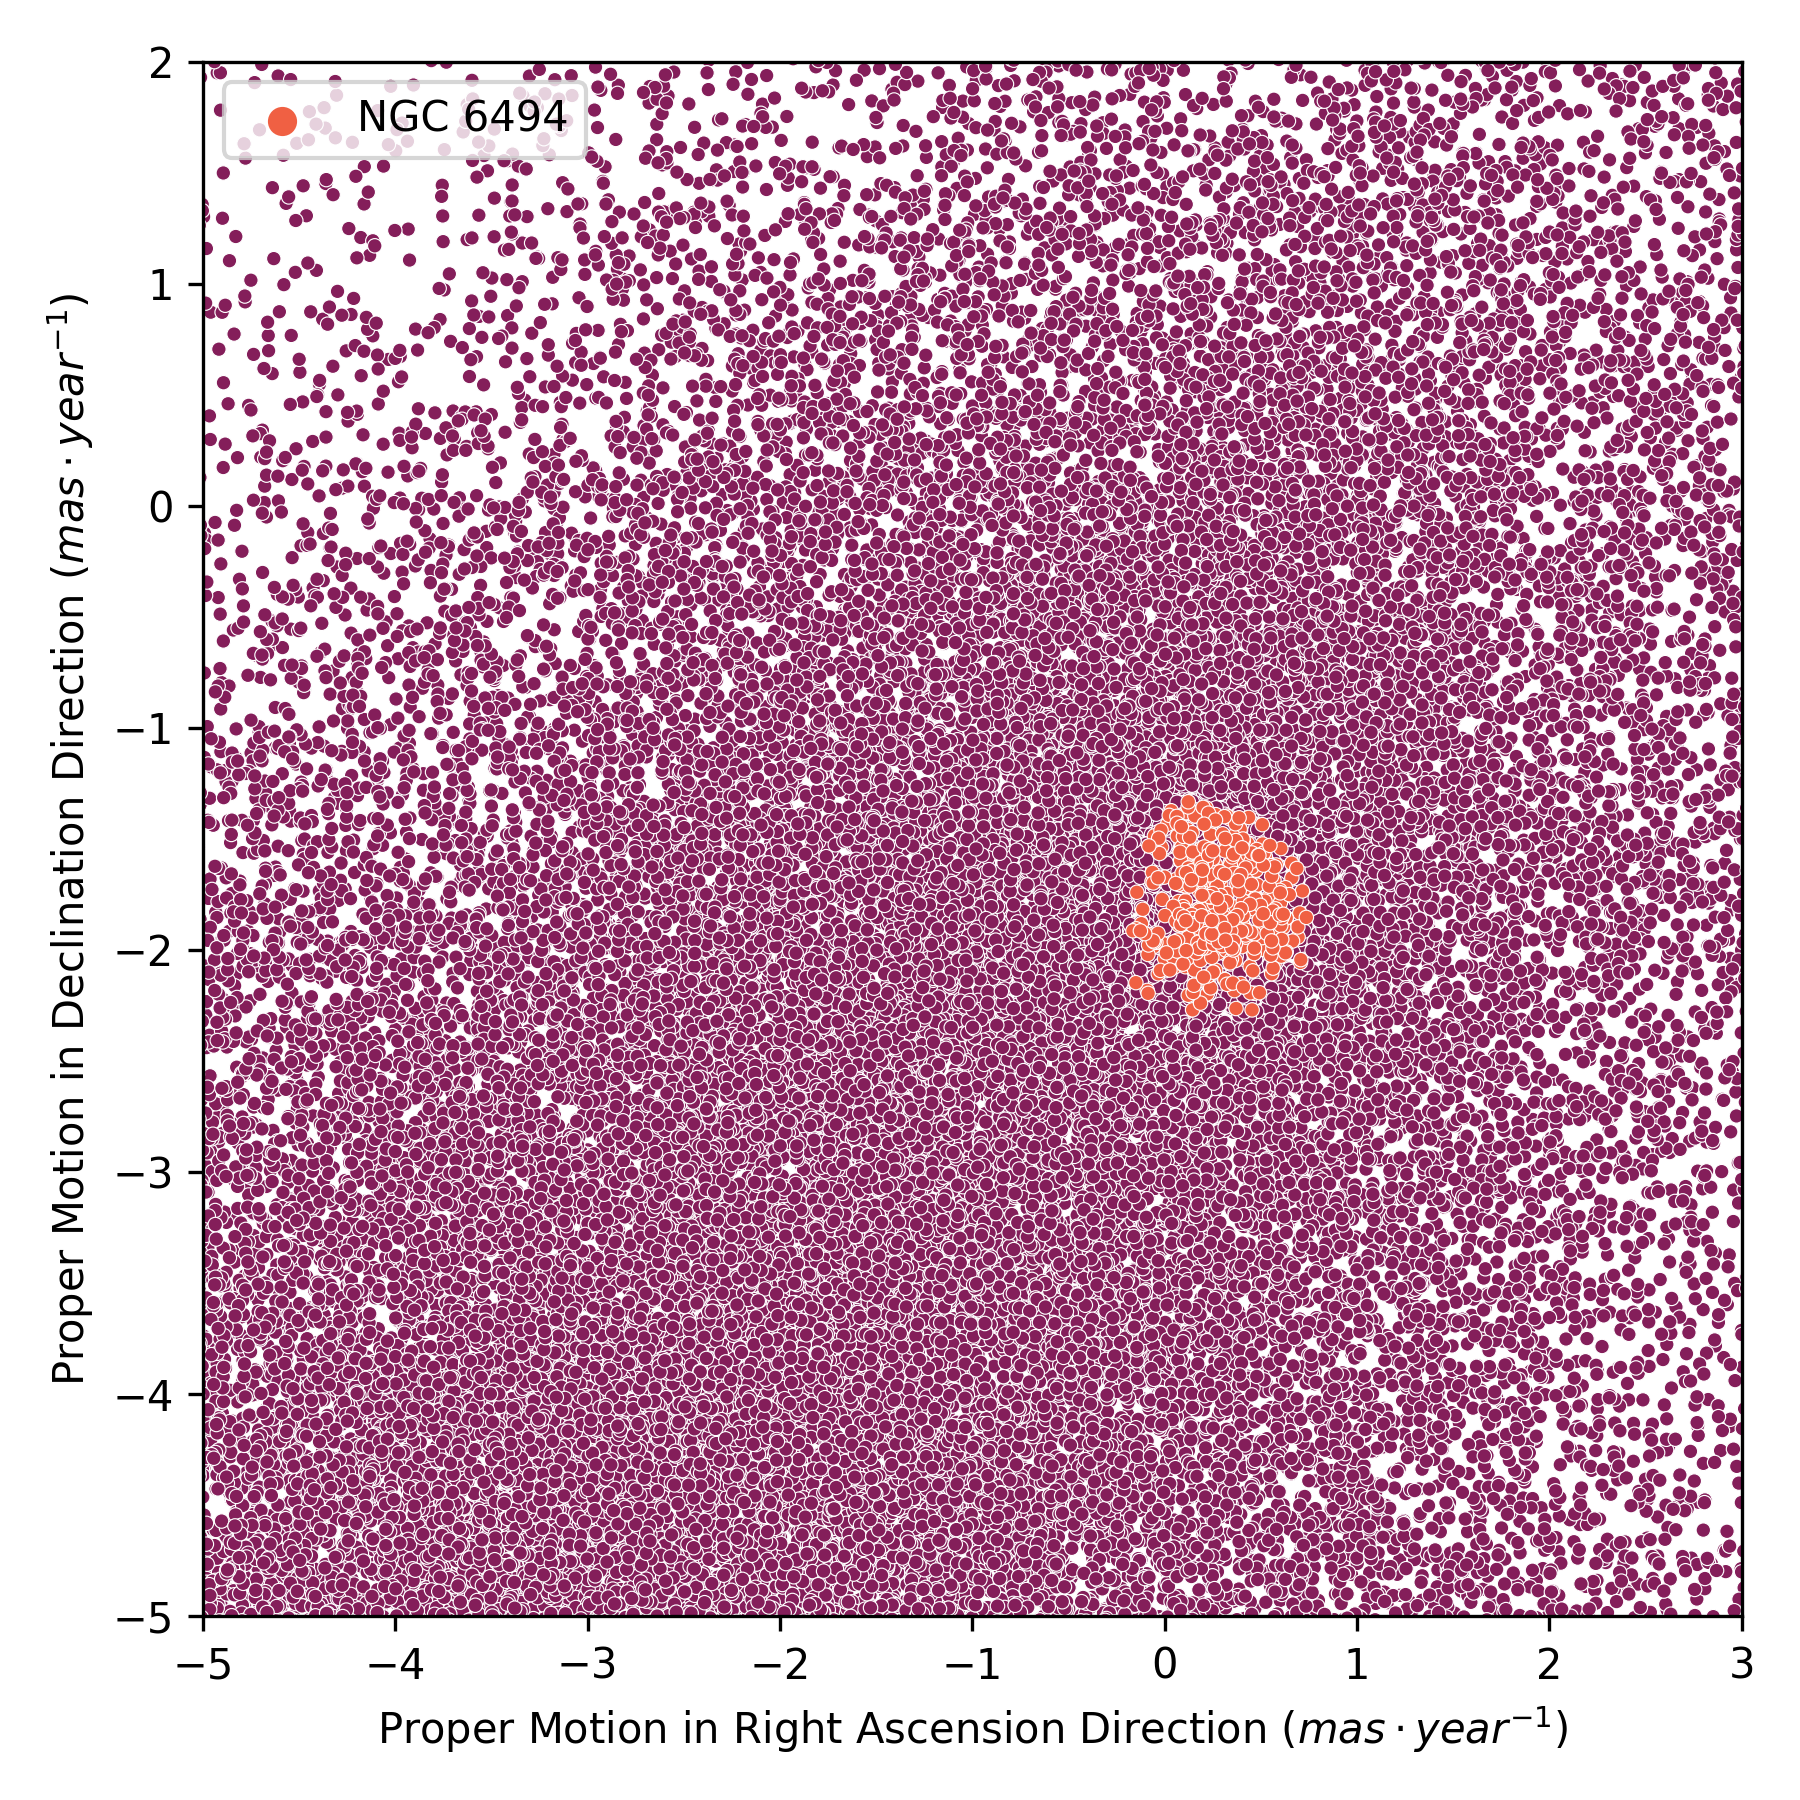
\includegraphics[width=\textwidth]{../figures/ngc_6494/pm_ngc_6494.png}
      \caption{Proper motions}
      \label{fig:pm_ngc_6494}
    \end{subfigure}
    \hfill
    \begin{subfigure}[t]{0.45\textwidth}
      \centering
      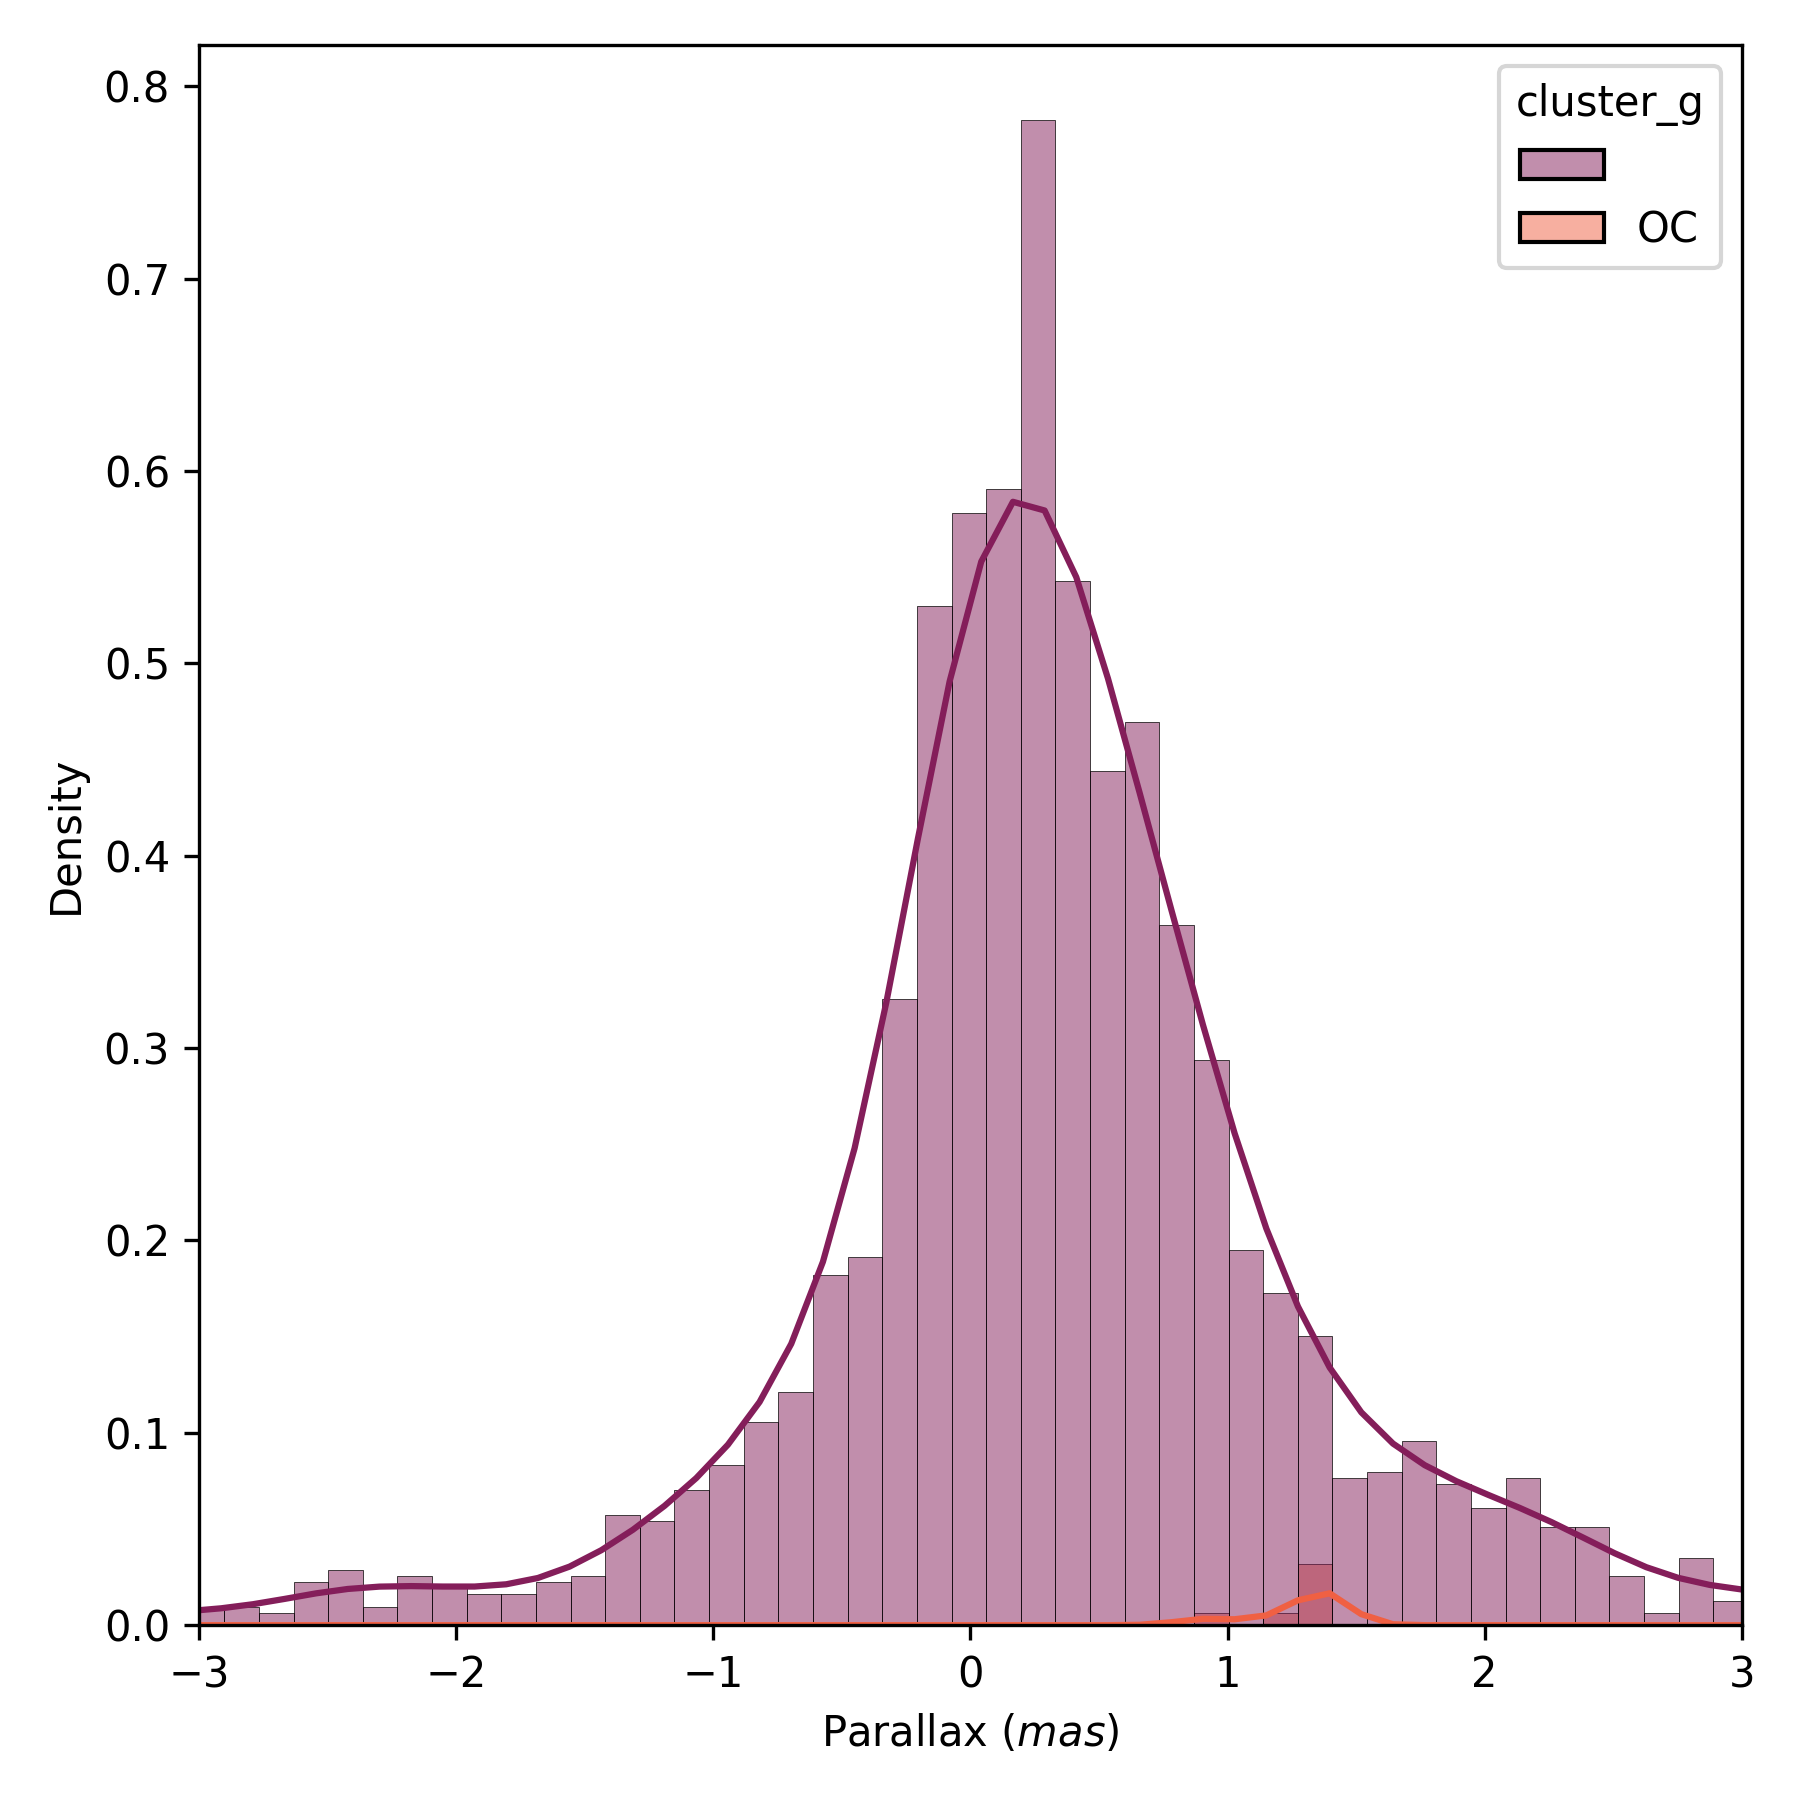
\includegraphics[width=\textwidth]{../figures/ngc_6494/parallax_ngc_6494.png}
      \caption{Parallax}
      \label{fig:parallax_ngc_6494}
    \end{subfigure}
  \end{subfigure}
  \caption{Open Cluster NGC 6494}
\end{figure}

At this point, it looks reasonable that the study of each individual cluster requires its own parametrization and technique
to identify it.

With Gaia DR2, which contains great quality astrometric and photometric data for a huge number of stars,
a new opportunity to simplify and optimize this processes is presented.
In this context new approaches are being developed to improve current detection methods and automate the OC characterization.
This work tries to take the best from \emph{Clusterix 2.0. A Virtual Observatory tool to estimate cluster membership probability}
\cite{balaguer2020clusterix} and \emph{Hunting for open clusters in Gaia DR2: 582 new open clusters
in the Galactic disc} \cite{castro2020hunting}, and merge them into a single \emph{machine learning}
tool capable of finding open clusters efficiently without requiring powerful machines to perform the computations.

The first one is a non-parametrized method. It determines empirically the frequency functions associated to astrometrical variables
without making any assumption about their profiles. However, it heavily does depend on the initial field selection and other
parameters related to frequency functions. \emph{Clusterix 2.0.} is a web app tool inside the Spanish Virtual Observatory
(VO) framework and works together with other VO tool such as:
\emph{TOPCAT} \cite{taylor2005topcat},
\emph{Aladin} \cite{bonnarel2000aladin},
\emph{VOSA} \cite{bayo2008vosa}, among other.

The second tool is based on Big Data techniques. Its purpose is to analyze the whole Gaia DR2 dataset looking for OCs by using
machine learning algorithms divided in two stages. In the first stage, the algorithm looks for posible OC candidates by searching
overdensities in the galactic disc.
The second stage studies candidates found in the first one by generating images with H-R diagrams and passing them
as sources to an Artificial Neural Network (ANN) which identifies isochrone patterns in photometric data (color and magnitude).
Before this approach was put into practice there were 1200 OCs known. Now, this number has been increased up to more than 2000 OCs
available at the Vizier catalogue \cite{ochsenbein2000vizier}.

The method developed in this project takes as base the approach made by \citeauthor{castro2020hunting} but rapidly diverges.
In first place, performance has been taken into account since the beginning, trying to get a reliable method without compromising the
needs of supercomputers.
To achieve this, instead of blindly analyzing the whole galactic disk a fields selection is made focusing in those regions with known OCs.
Then, these fields are analyzed with an homogeneous methodology based on machine learning algorithms using as sources astrometric and
photometric variables. The goal is the characterization of each individual star in the cluster, discerning wether the star belongs the OC
or not.

Thus, the main goal of this project is not the discovery of new open clusters or even candidates, but the development of a model that,
applied to already known open clusters, allows us the characterization of those OCs on an unsupervised way, with a reasonable computing
power and taking into account the same selection of astrometric and photometric variables for every OC.

% TODO: Concluir con una última sección de resumen de conclusiones, resumiendo las principales averiguaciones del estudio del dominio
% y cómo van a afectar al desarrollo específico del trabajo.

\chapter{Method}

In this chapter we address the different steps followed to perform the creation of the unsupervised clustering model for open cluster characterization.

All code has been developed with the Python programming language \cite{Python3}. Other auxiliary tools like \emph{Docker} \cite{merkel2014docker},
\emph{PostgreSQL} \cite{postgresql}, \emph{Jupyter Notebooks} \cite{Kluyver2016jupyter}, and frameworks such as \emph{Astropy} \cite{astropy:2013} \cite{astropy:2018},
\emph{Scikit-Learn} \cite{scikit-learn}, \emph{Seaborn} \cite{michael_waskom_2017_883859}, \emph{SQLAlchemy} \cite{sqlalchemy} and
\emph{Keras} \cite{chollet2015keras} have been used too.

\begin{figure}[htbp]
  \centering
  \begin{subfigure}{0.5\textwidth}
    \centering
    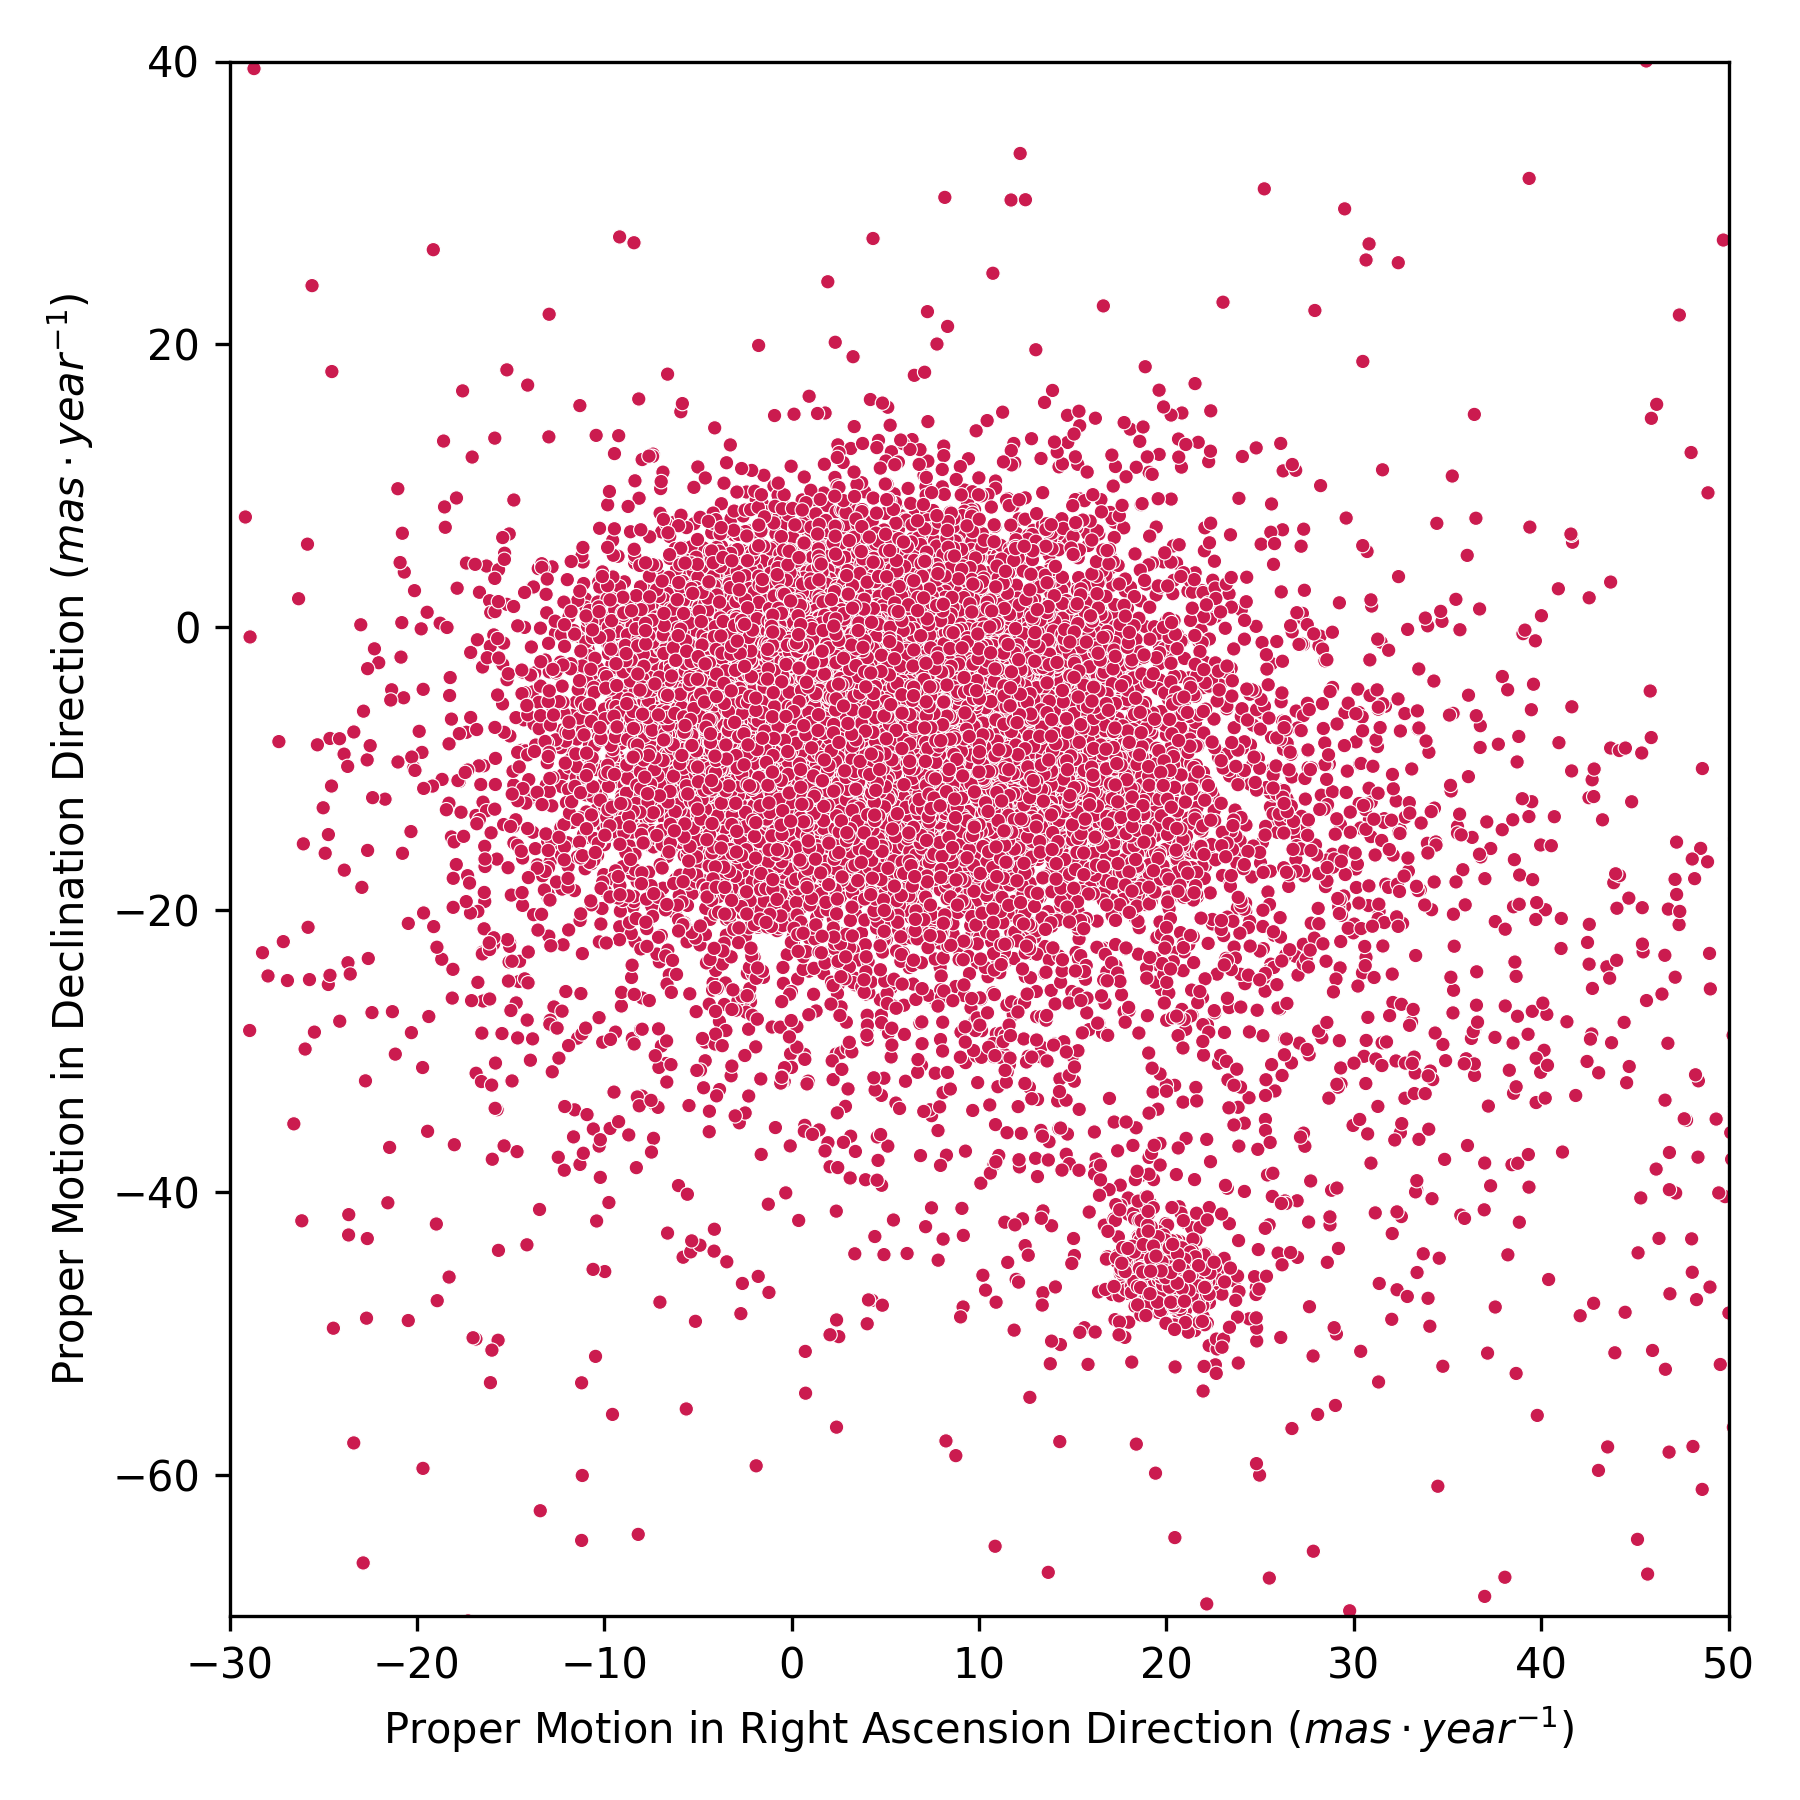
\includegraphics[width=\textwidth]{../figures/melotte_22/raw_pm_melotte_22.png}
  \end{subfigure}
  \caption{Melotte 22 proper motions}
  \label{fig:raw_pm_melotte_22}
\end{figure}

For the sake of simplicity, we are taking \emph{Melotte 22 (Messier 45)} \cite{elsanhoury2019ppmxl} to illustrate the whole method. This cluster is well studied
and their stars are not too mixed with other region stars.

Figure \ref{fig:raw_pm_melotte_22} shows \emph{proper motions in right ascension and declination} for a sample of the downloaded dataset for Melotte 22.
At first sight, two main clusters can be distinguished, one of them centered nearly at (0, 0) and the second cluster with center at (20, -45). This second cluster
is the one we are looking for.

However, although this second cluster is almost isolated, there are stars that do not belong to the OC. Thus, we need more information to properly characterize the OC.

\begin{figure}[htbp]
  \centering
  \begin{subfigure}{0.9\textwidth}
    \centering
    \begin{subfigure}[t]{0.45\textwidth}
      \centering
      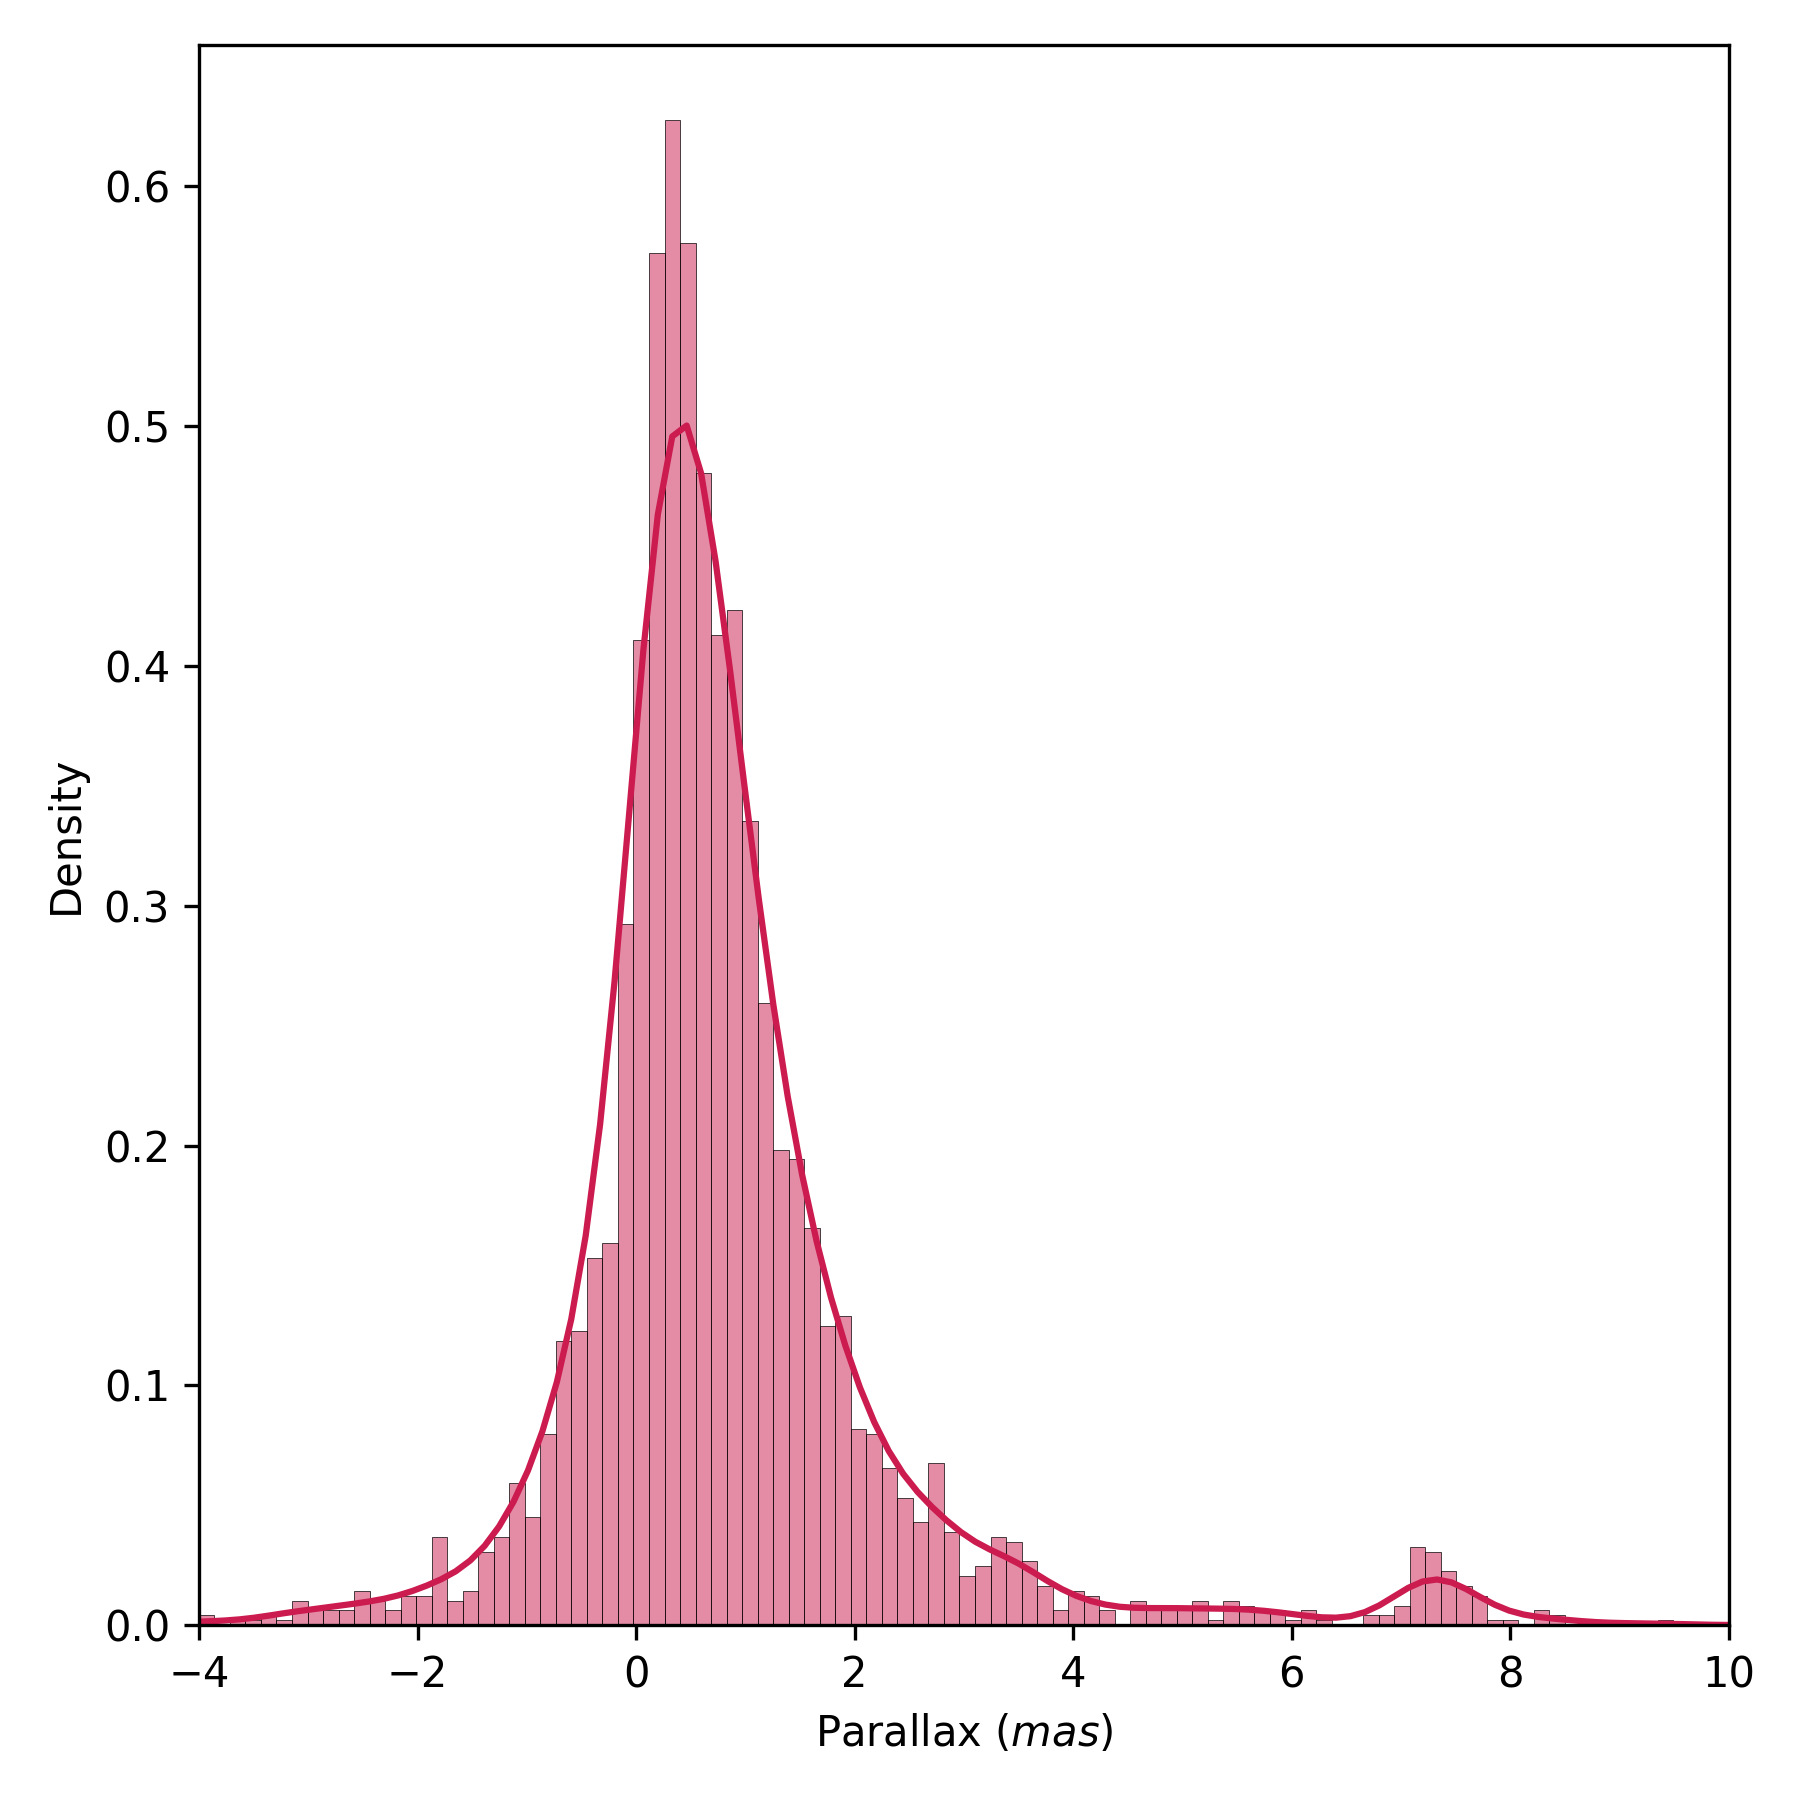
\includegraphics[width=\textwidth]{../figures/melotte_22/raw_parallax_melotte_22.png}
    \end{subfigure}
    \hfill
    \begin{subfigure}[t]{0.45\textwidth}
      \centering
      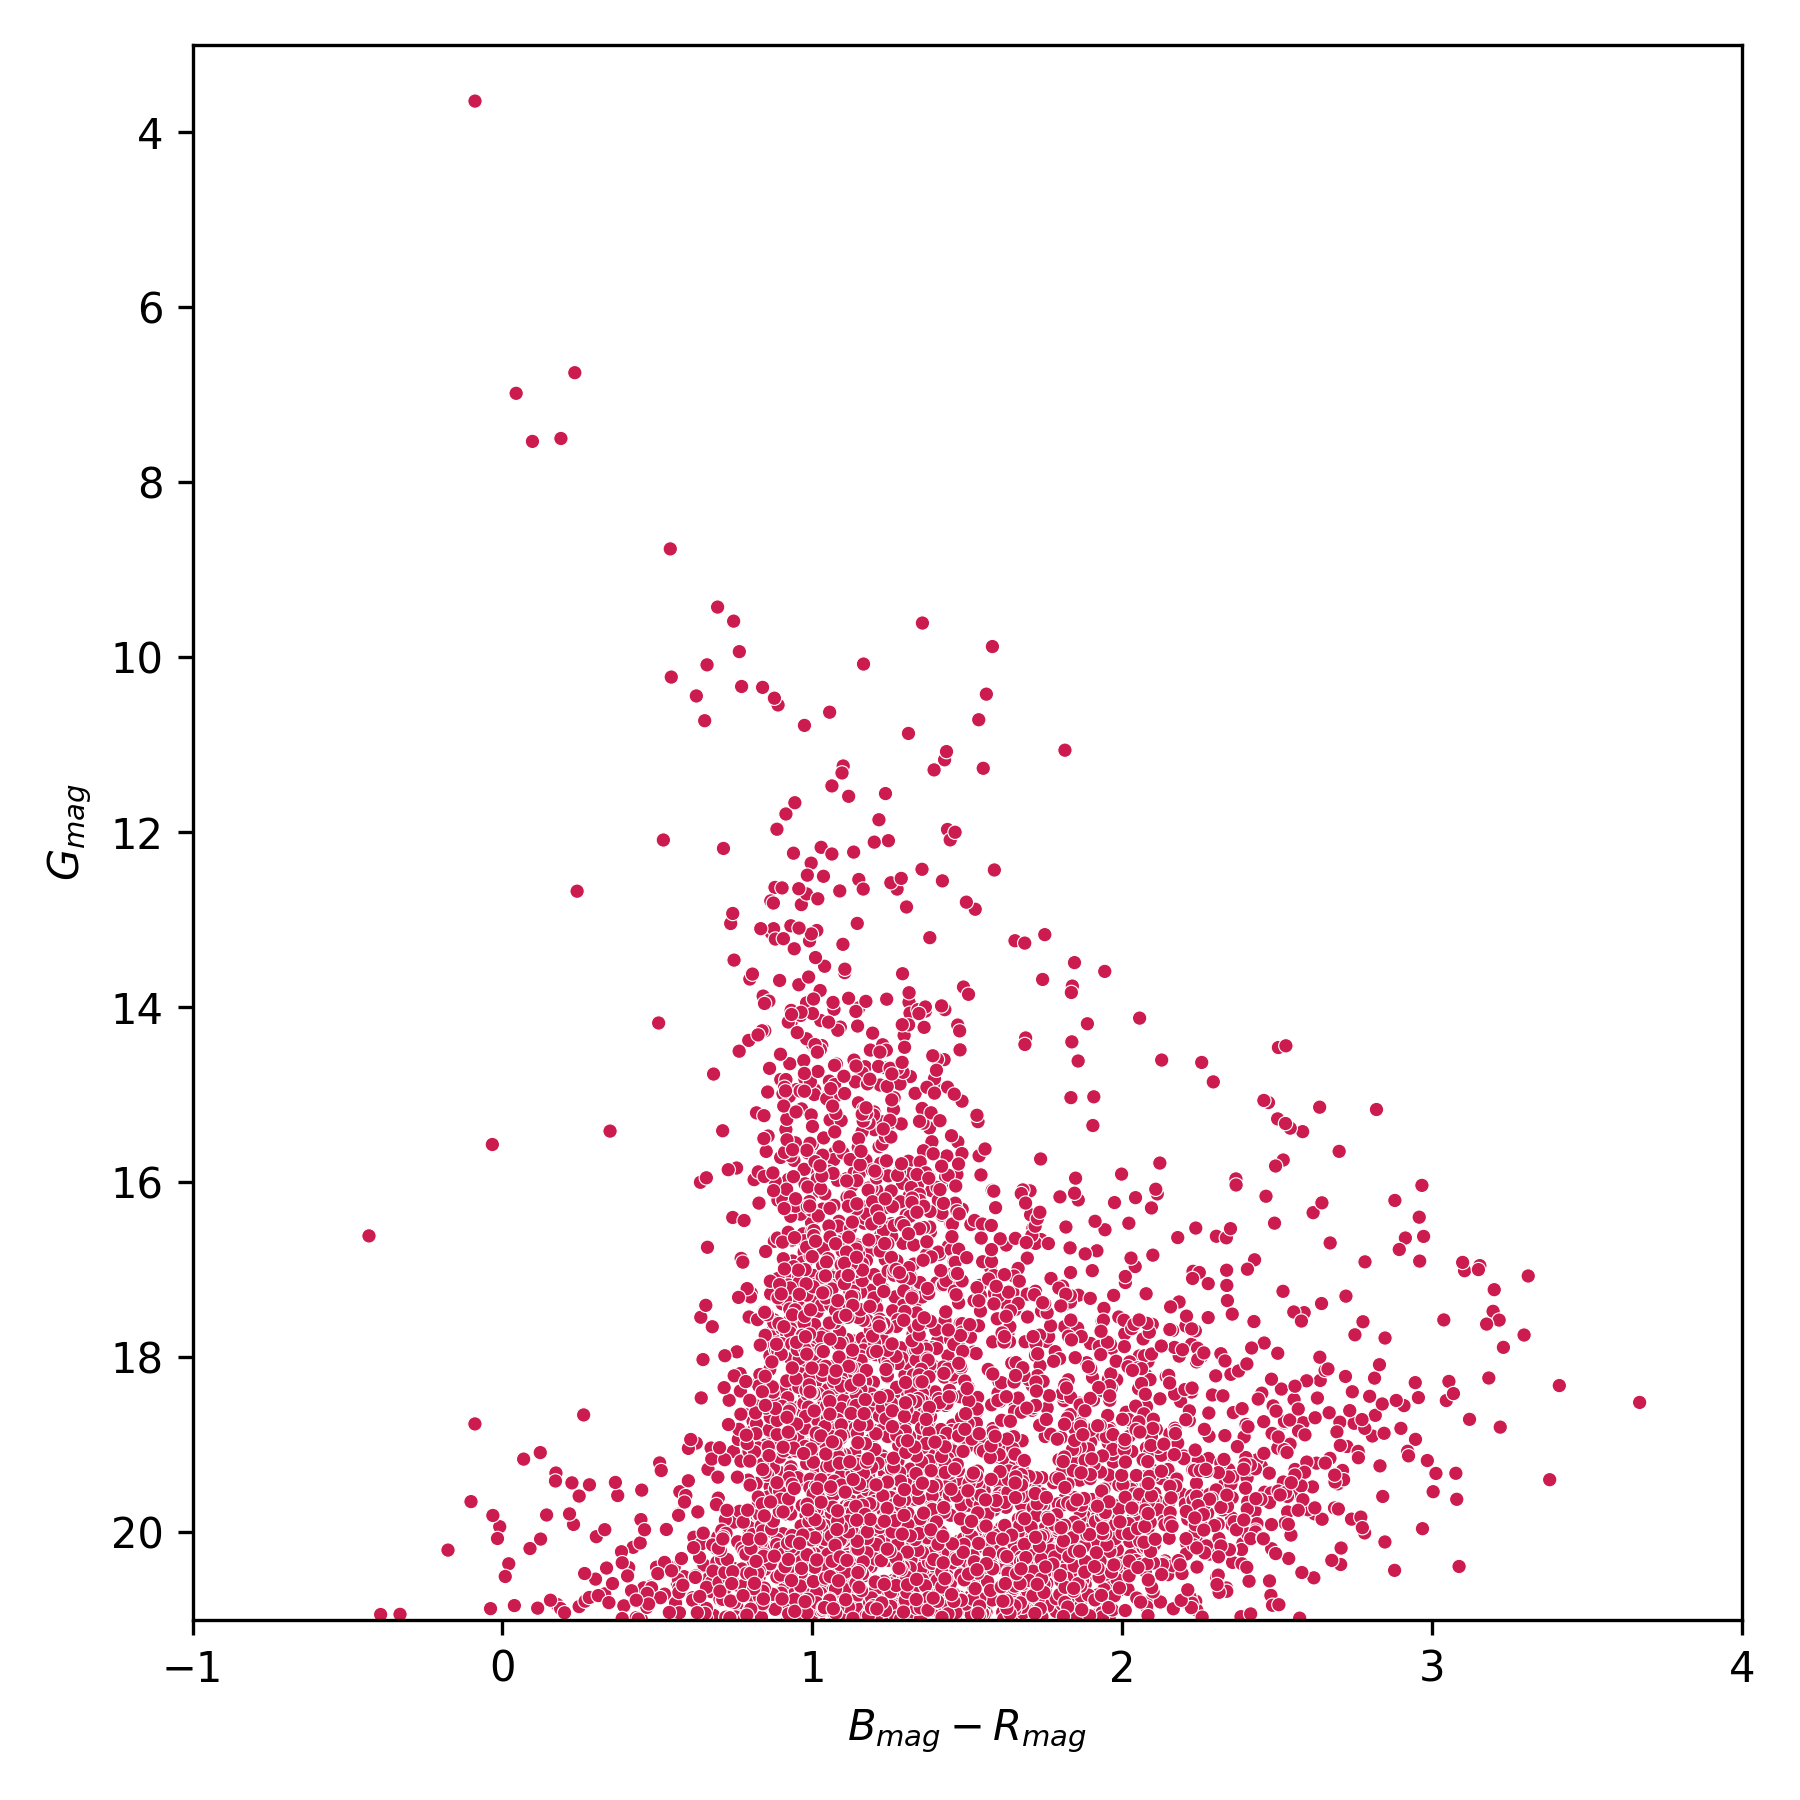
\includegraphics[width=\textwidth]{../figures/melotte_22/raw_hr_diagram_melotte_22.png}
    \end{subfigure}
  \end{subfigure}
  \caption{Melotte 22 parallax and H-R diagram}
  \label{fig:raw_parallax_hr_diagram_mellote_22}
\end{figure}

Figure \ref{fig:raw_parallax_hr_diagram_mellote_22} shows the parallax histogram and the H-R diagram for this cluster, respectively.

The figure on the left shows a resonance at $\approx 7.3mas$ belonging the OC. While the figure on the right would help us to look for isochrone curves and so,
to determine the age of these stars.

\section{Data Mining}

Before being able to develop and test our clustering model, the first step is to download the required data from Gaia repository
and store it in a custom database for later access.

Due to the large amount of data available at Gaia, a complete download is not viable neither useful.
In order to reduce the size of the dataset to be downloaded, the OpenClust catalogue \cite{dias2002new} (Figure \ref{fig:OpenClustComplete})
has been used to restrict the sky regions to be explored.

This download is not limited to the size registered in the catalogue. Instead, a wider region is downloaded for each cluster to include
stars outside the cluster. The idea is that the unsupervised model must be able to clusterize the stars that belongs to the OC and to discard
those outsiders when characterizing the open cluster.

\begin{figure}[htbp]
  \centering
  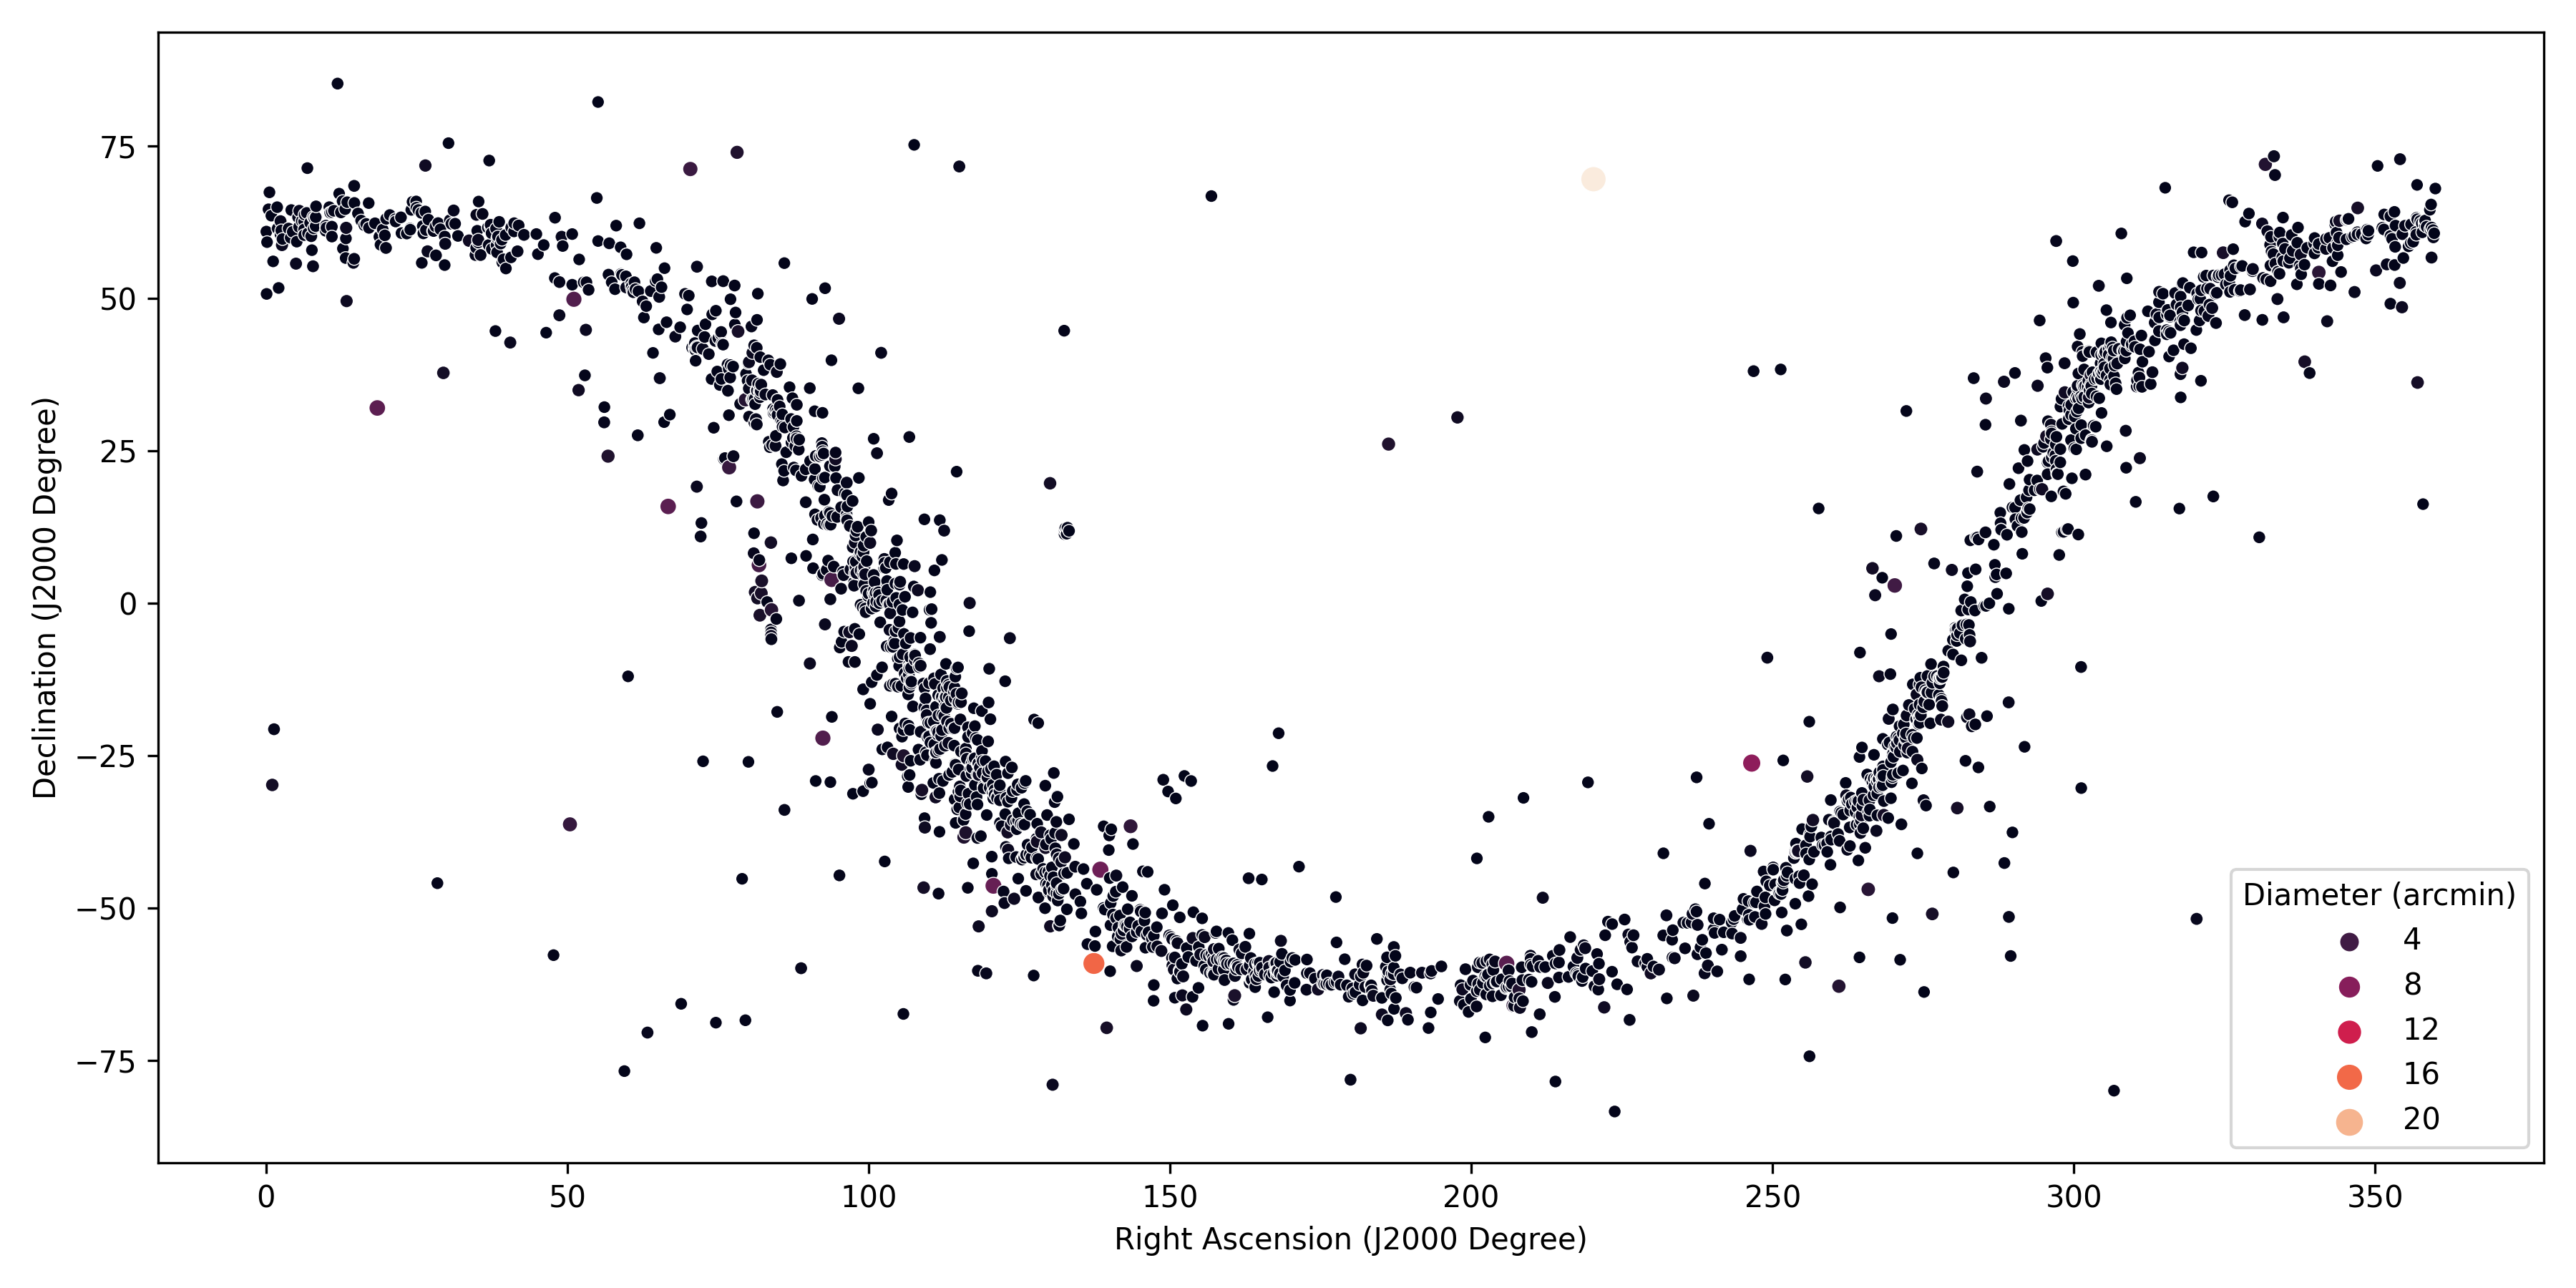
\includegraphics[width=0.9\textwidth]{../figures/openclust_catalogue.png}
  \caption{OpenClust Catalogue Distribution}
  \label{fig:OpenClustComplete}
\end{figure}

Taking these considerations into account, the downloaded dataset covers nearly 114 million stars (42GB of compressed data). This dataset is significantly
smaller than the whole Gaia DR2 dataset, which contains information for approximately 1,600 million stars. However, it is still being too large.

Since not all the downloaded clusters are good enough, we will apply a series of filters to discard clusters which do not have enough stars or contain too
many \emph{null} values.

So, a cluster must fulfil the following filters to be accepted:

\begin{itemize}
  \item Cluster diameter above 25.0 arcmin
  \item Parallax absolute value greater than 0.0
  \item Number of stars\footnote{Every star must have all required features completely defined, i.e. without null values} in the selected region above 40,000 stars
\end{itemize}

As shown in Figure \ref{fig:OpenClustSelection}, these constrains give us a smaller dataset but it is still being a good representation of all clusters in the Milky Way
since they are equally distributed around the galaxy disk.

After having applied these filters, the number of cluster to analyse is 169 with nearly 75 million stars.

Since we have set no upper limit to the number of stars inside a cluster, for the sake of simplicity and as a commitment to the project delivery dates
and the available computing power, smaller clusters will be preferred over the greatest ones.

As an extension of this work, the designed model could be applied to a region not covered by these constrains for a later understanding of the results.

\begin{figure}[htbp]
  \centering
  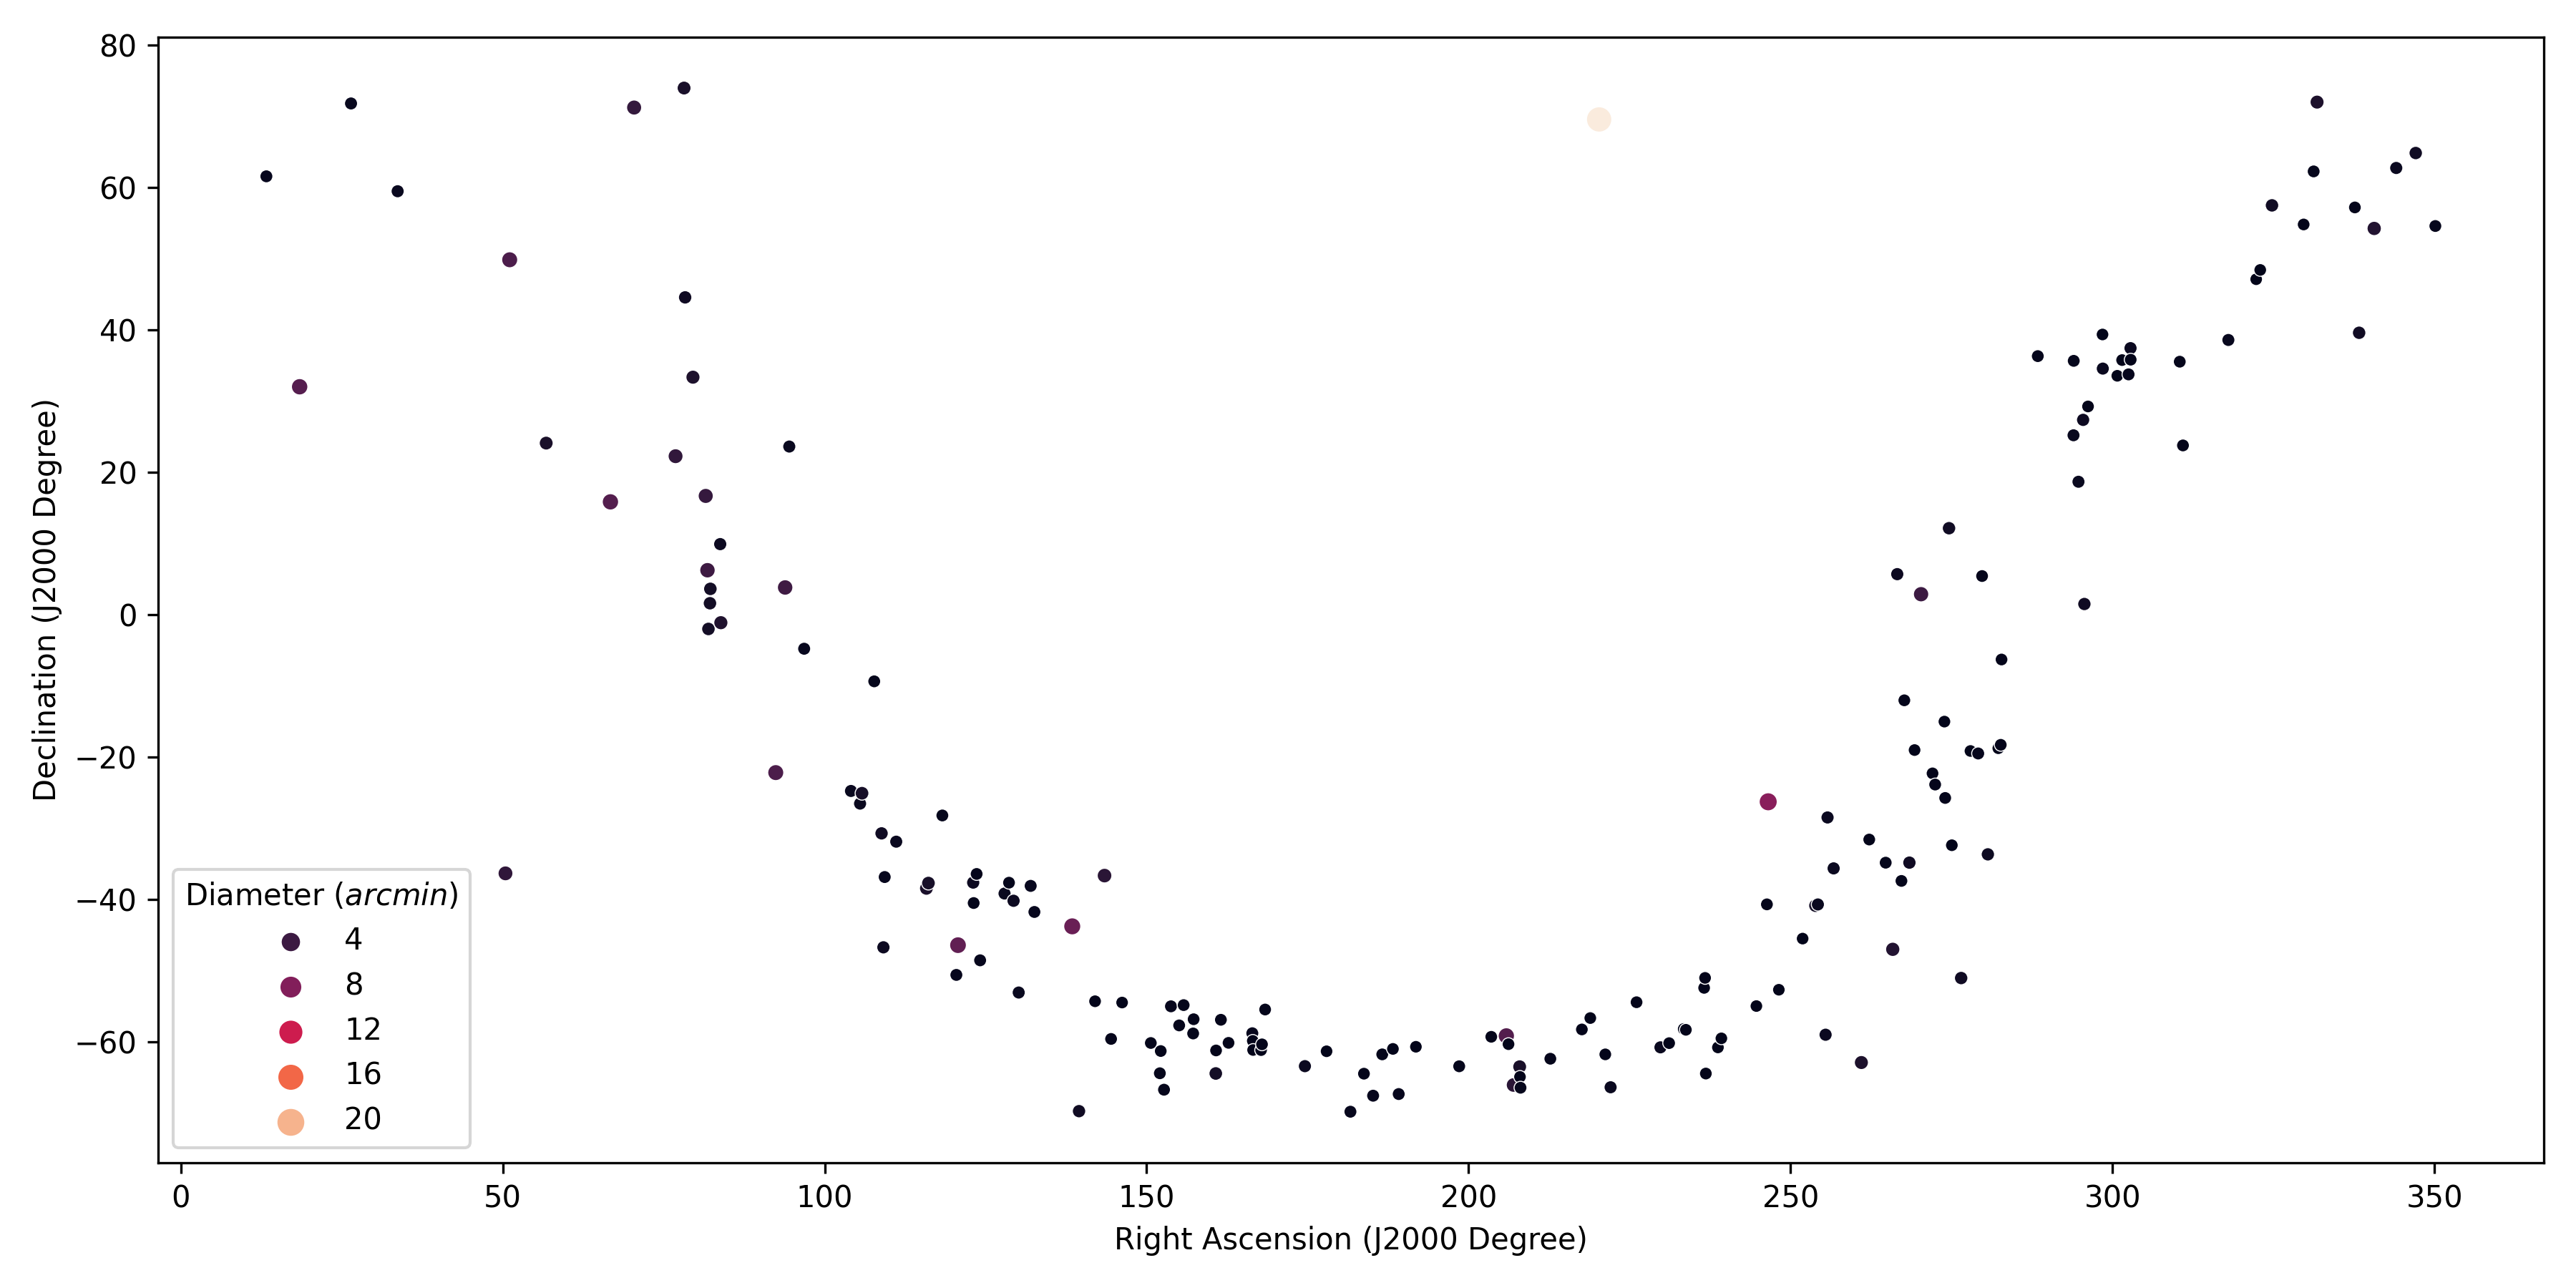
\includegraphics[width=0.9\textwidth]{../figures/cluster_selection_tier1.png}
  \caption{OpenClust Catalogue Selection Distribution}
  \label{fig:OpenClustSelection}
\end{figure}

\subsection{Download Process}

The download process has been performed with two Docker containers: a \emph{downloader} and the \emph{database}.

The first one is a container built from a \verb|python:3.8| image that contains the \verb|cdalvaro| package and the \verb|downloader.py| script.
This script is prepared to load the OpenClust catalogue, connect to the Gaia DR2 database, download all stars contained inside each cluster
(with a radius multiplier to increase the area to be downloaded) and save the downloaded data inside our custom database hosted in the second container.

\verb|downloader.Dockerfile| contains the build instructions for the downloader image. We use \href{https://github.com/features/actions}{GitHub Actions}
for automating the process of building a new version of the image with every new push made to the \verb|main| branch.

This image can be pulled from the \href{https://github.blog/2020-09-01-introducing-github-container-registry/}{GitHub Container Registry}:

\begin{minted}{sh}
  docker pull ghcr.io/cdalvaro/gaia-downloader:latest
\end{minted}

The second container is just a \verb|postgres:12.4| image which loads an initial script when the database is not yet initialized for creating the
database schema. This container is used later as the main database for data analysis.

The database has two main tables in \verb|public| schema:

\begin{itemize}
  \item \verb|regions| for storing cluster properties such as \emph{location}, \emph{diameter} and other properties
  \item \verb|gaiadr2_source| which contains data for all downloaded stars from Gaia
\end{itemize}

The second table is partitioned by region, storing all stars related to one cluster inside an independent table for optimized access performance.

Methods for retrieving information from the database are available through an instance of \verb|cdalvaro.DB|. This class contains methods
for recovering stars information for a given region as a Pandas \verb|DataFrame| ready for data analysis.

These containers are orchestrated with a \verb|docker-compose.yml| file which automatically launches one instance of each container.

The developed code for this work can be found inside the \verb|src| directory at GitHub:
\href{https://github.com/cdalvaro/machine-learning-master-thesis}{cdalvaro/machine-learning-master-thesis} repository.

\section{Feature Selection}
\label{sec:feature_selection}

As mentioned before, we want our model to characterize open clusters by looking at their dynamics properties.

Also, we want to maintain as simple as possible our clustering model in order to avoid requiring too much computing resources.

Proper motion in right ascension and declination seems like a natural choice since, as we know, stars belonging to the same OC share a common motion vector.

Parallax is another important feature. It lets us know how far stars are from us. And, since all stars within an open cluster were born from the same dust cloud,
they must all have similar parallax.

However, we are not going to use these raw features. Instead, we are taken a combination of them.

First, we correct proper motion in right ascension and declination by dividing them by the parallax. That way we normalize these quantities and help our clustering
models to improve their performance.

Another computed property that we are considering is the modulus of the proper motion. That way, we relate both features and therefore force our model to keep them tight.

\begin{figure}[htbp]
  \centering
  \begin{subfigure}{0.9\textwidth}
    \centering
    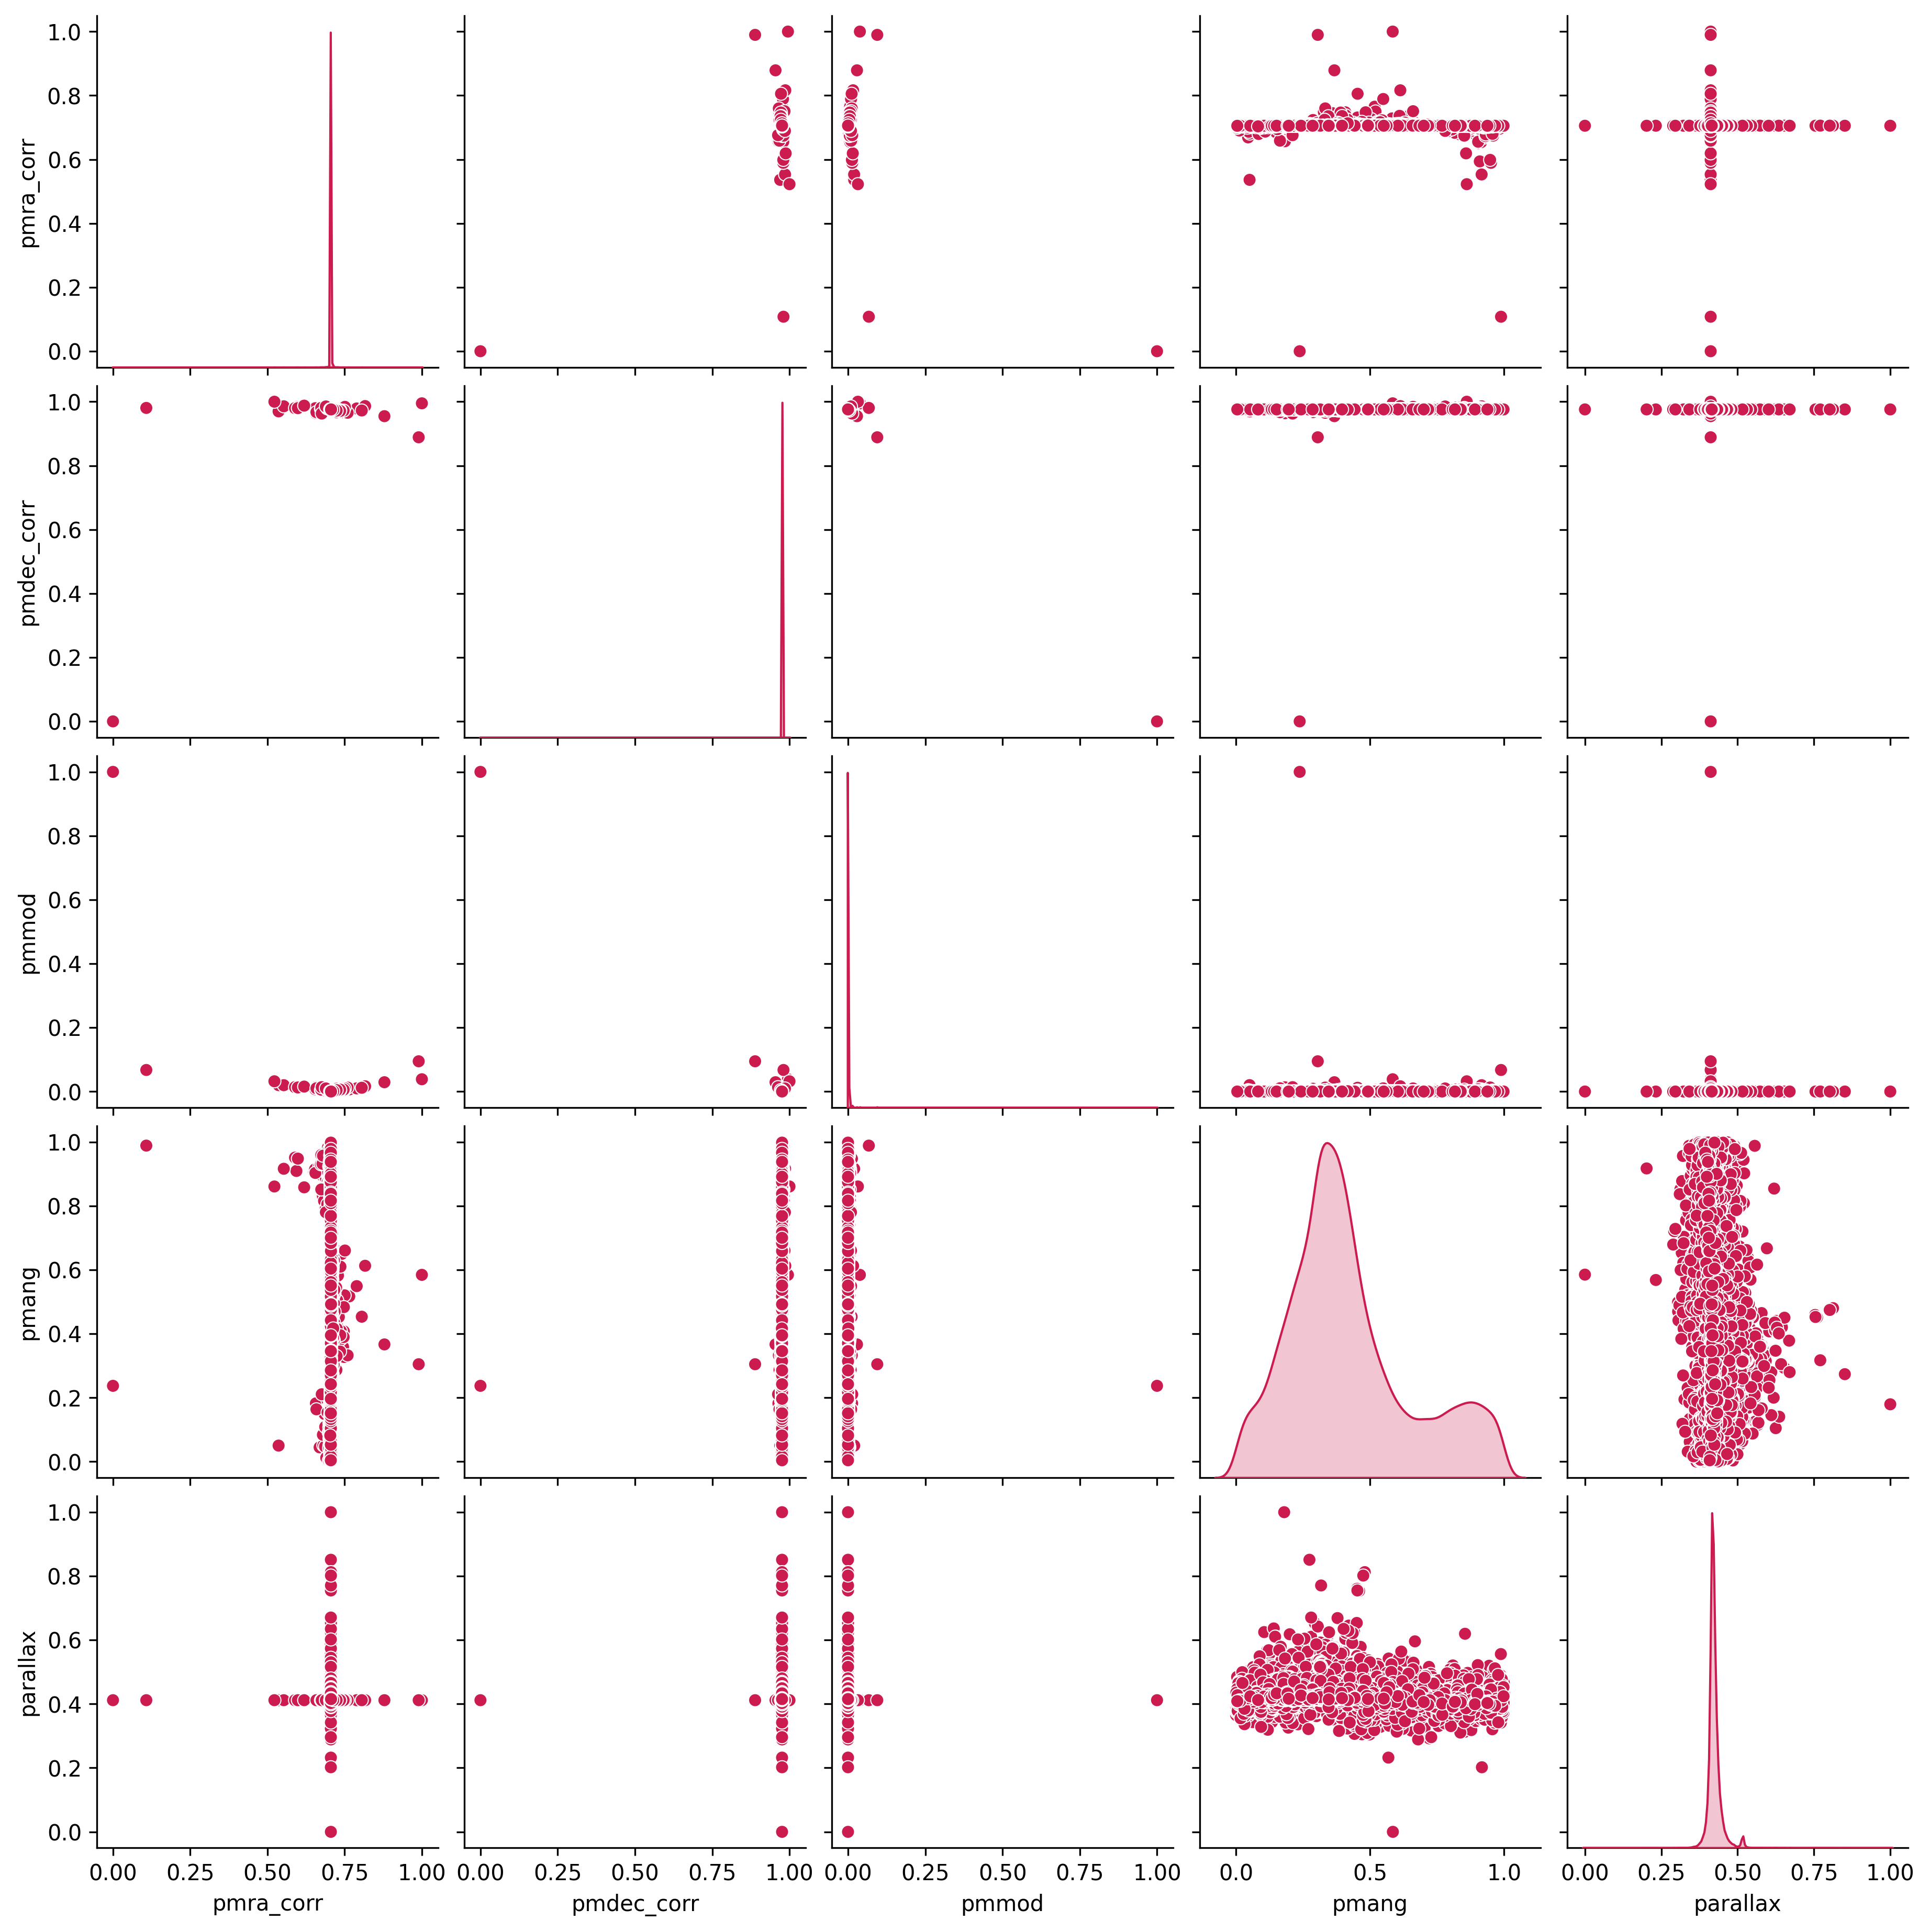
\includegraphics[width=\textwidth]{../figures/melotte_22/features_melotte_22.png}
  \end{subfigure}
  \caption{Melotte 22 feature pairplot}
  \label{fig:features_melotte_22}
\end{figure}

So, in summary, these are the features we are going to use as sources for our clustering models:

\begin{itemize}
  \item \emph{Proper motion in right ascension} (corrected by parallax): $\mu_{\alpha}$
  \item \emph{Proper motion in declination} (corrected by parallax): $\mu_{\delta}$
  \item \emph{Parallax}: $\varpi$
  \item \emph{Proper motion modulus}: $\left\| \vec{\mu} \right\|$
\end{itemize}

This feature selection has been refined by iterating over the K-Means clustering process with a fixed number of clusters and varying the feature selection in each case.
The final selection is the one with best \emph{silhouette score} \cite{rousseeuw1987silhouettes}.

The silhouette score is a metric used to determine how good a cluster is based on intra-cluster distances and nearest-cluster distances.
The best possible value is 1, and the worst is -1. Negative values mean that some samples have been assigned to the wrong cluster.

This process is explained in more detail in Appendix \ref{chap:feature_selection}.

\section{Soft Clustering with K-Means}

Once we have found the set of features that best describes our problem, we can begin searching for the OC in the study region.

Our first approach to find the open cluster within the region of interest is to use the K-Means algorithm.

Since we are looking for a single cluster, it seems reasonable to use a clustering algorithm and set it to find two clusters.
One for the desired OC and another which contains stars that do not belong to the open cluster.
However, this idea is not completely right.

\begin{figure}[htbp]
  \centering
  \begin{subfigure}{0.9\textwidth}
    \centering
    \begin{subfigure}[t]{0.3\textwidth}
      \centering
      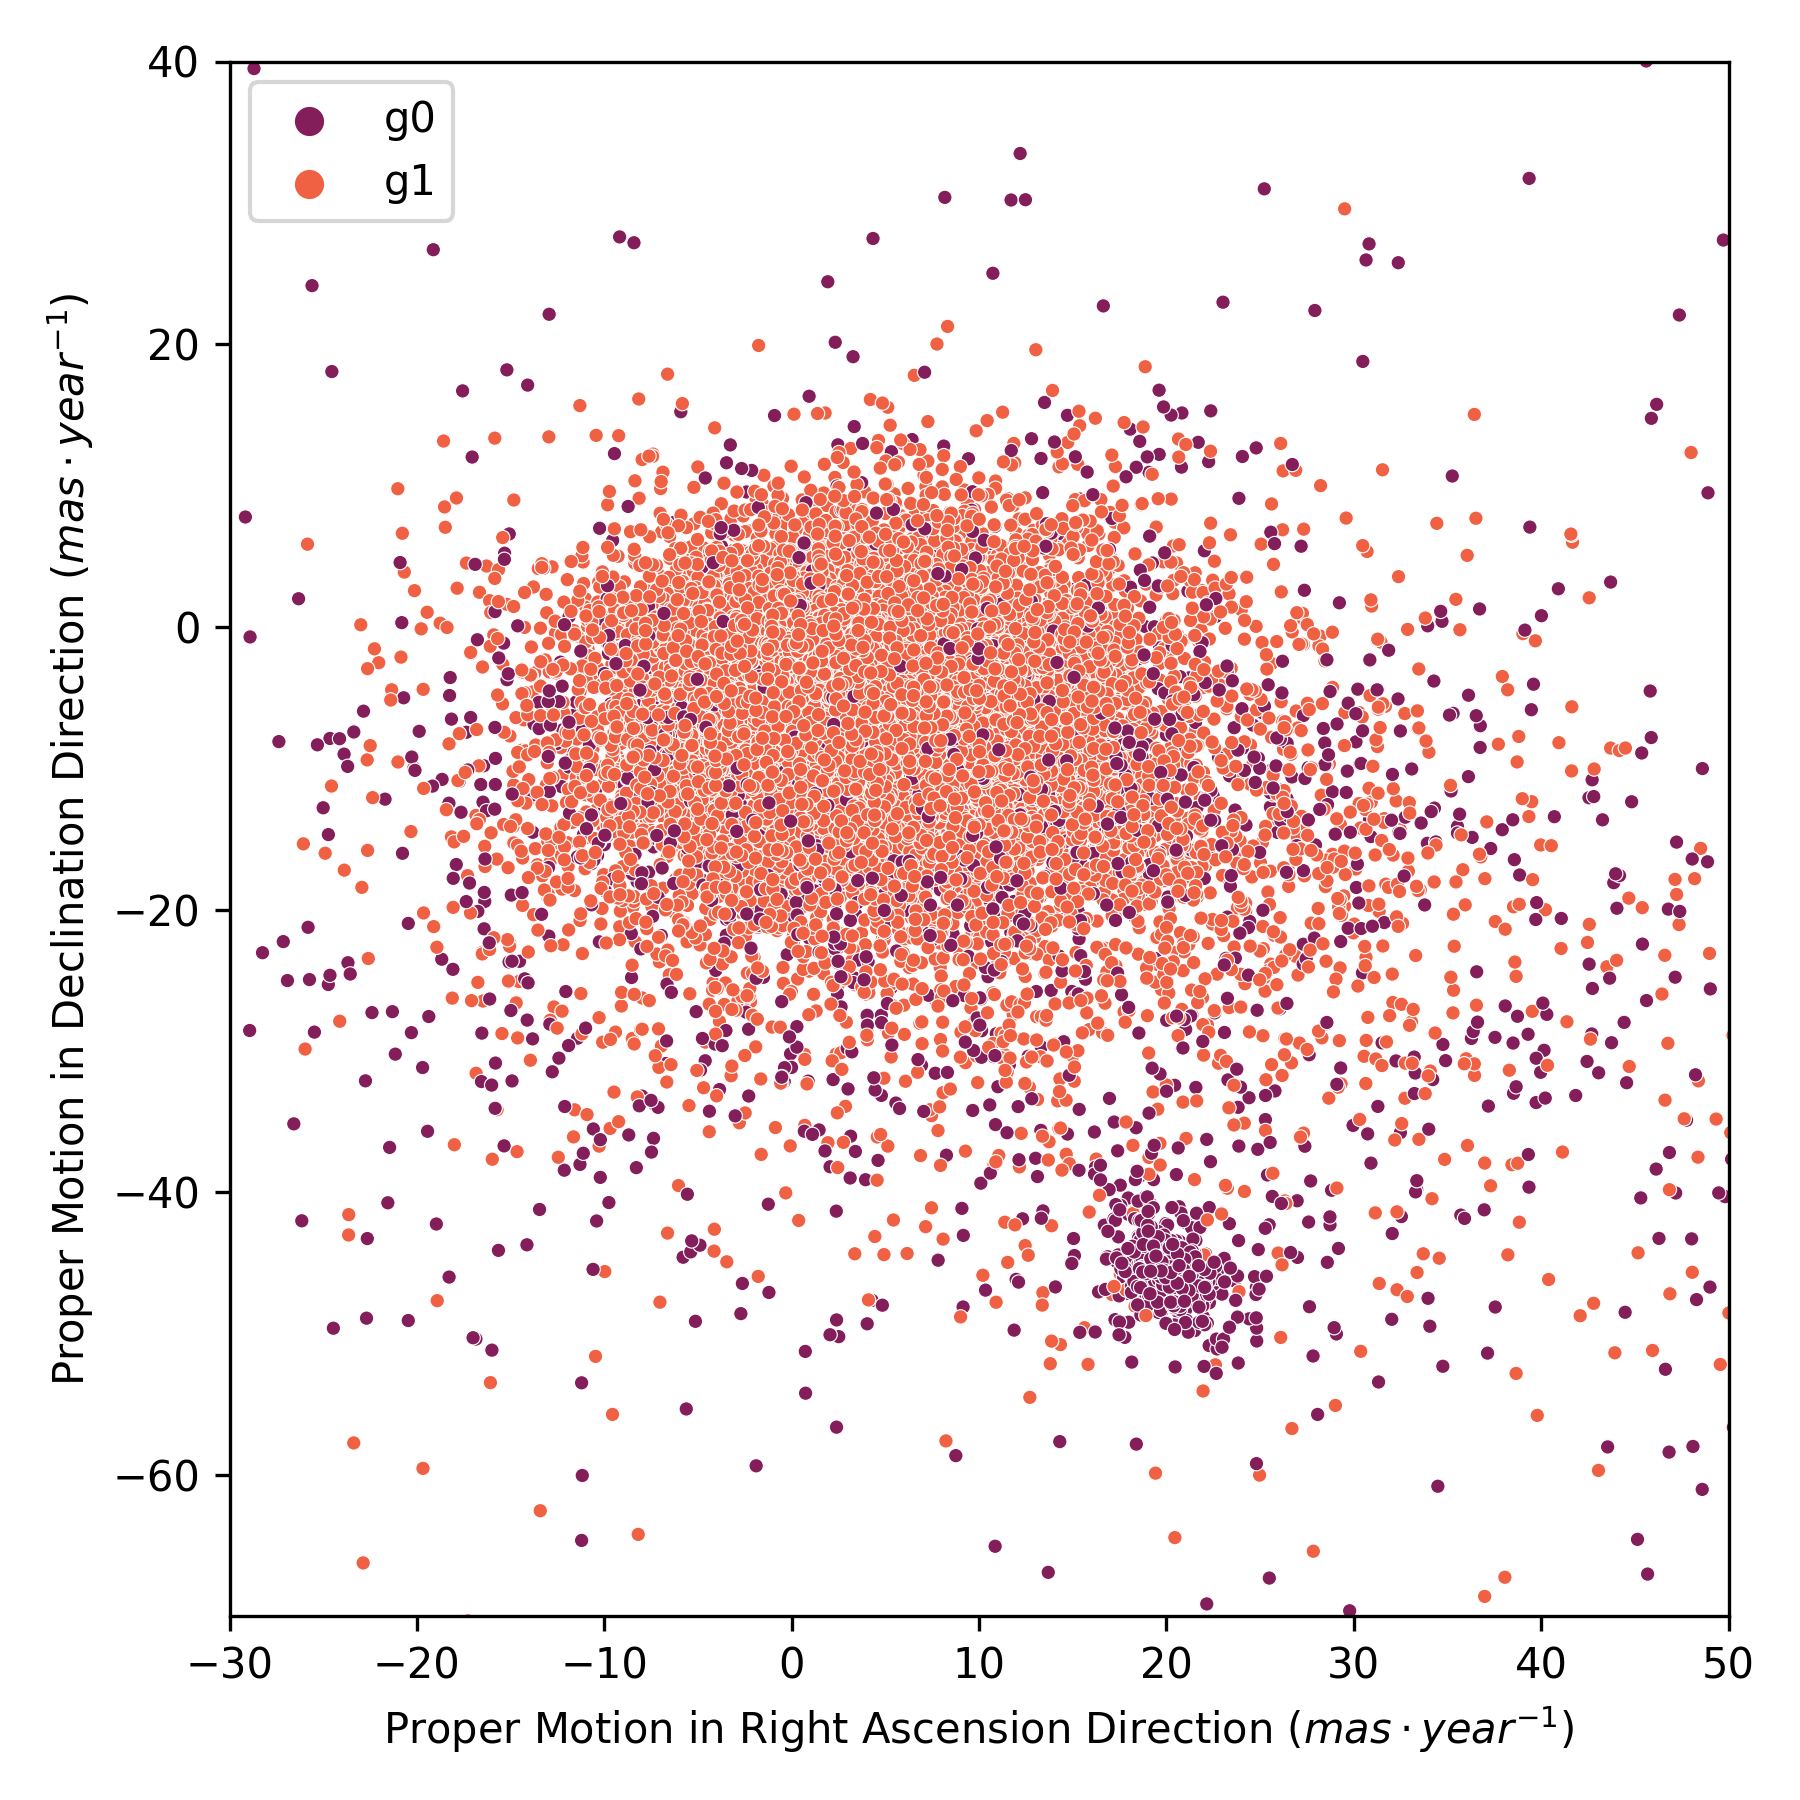
\includegraphics[width=\textwidth]{../figures/kmeans/kmeans_n2_pm_melotte_22.png}
    \end{subfigure}
    \hfill
    \begin{subfigure}[t]{0.3\textwidth}
      \centering
      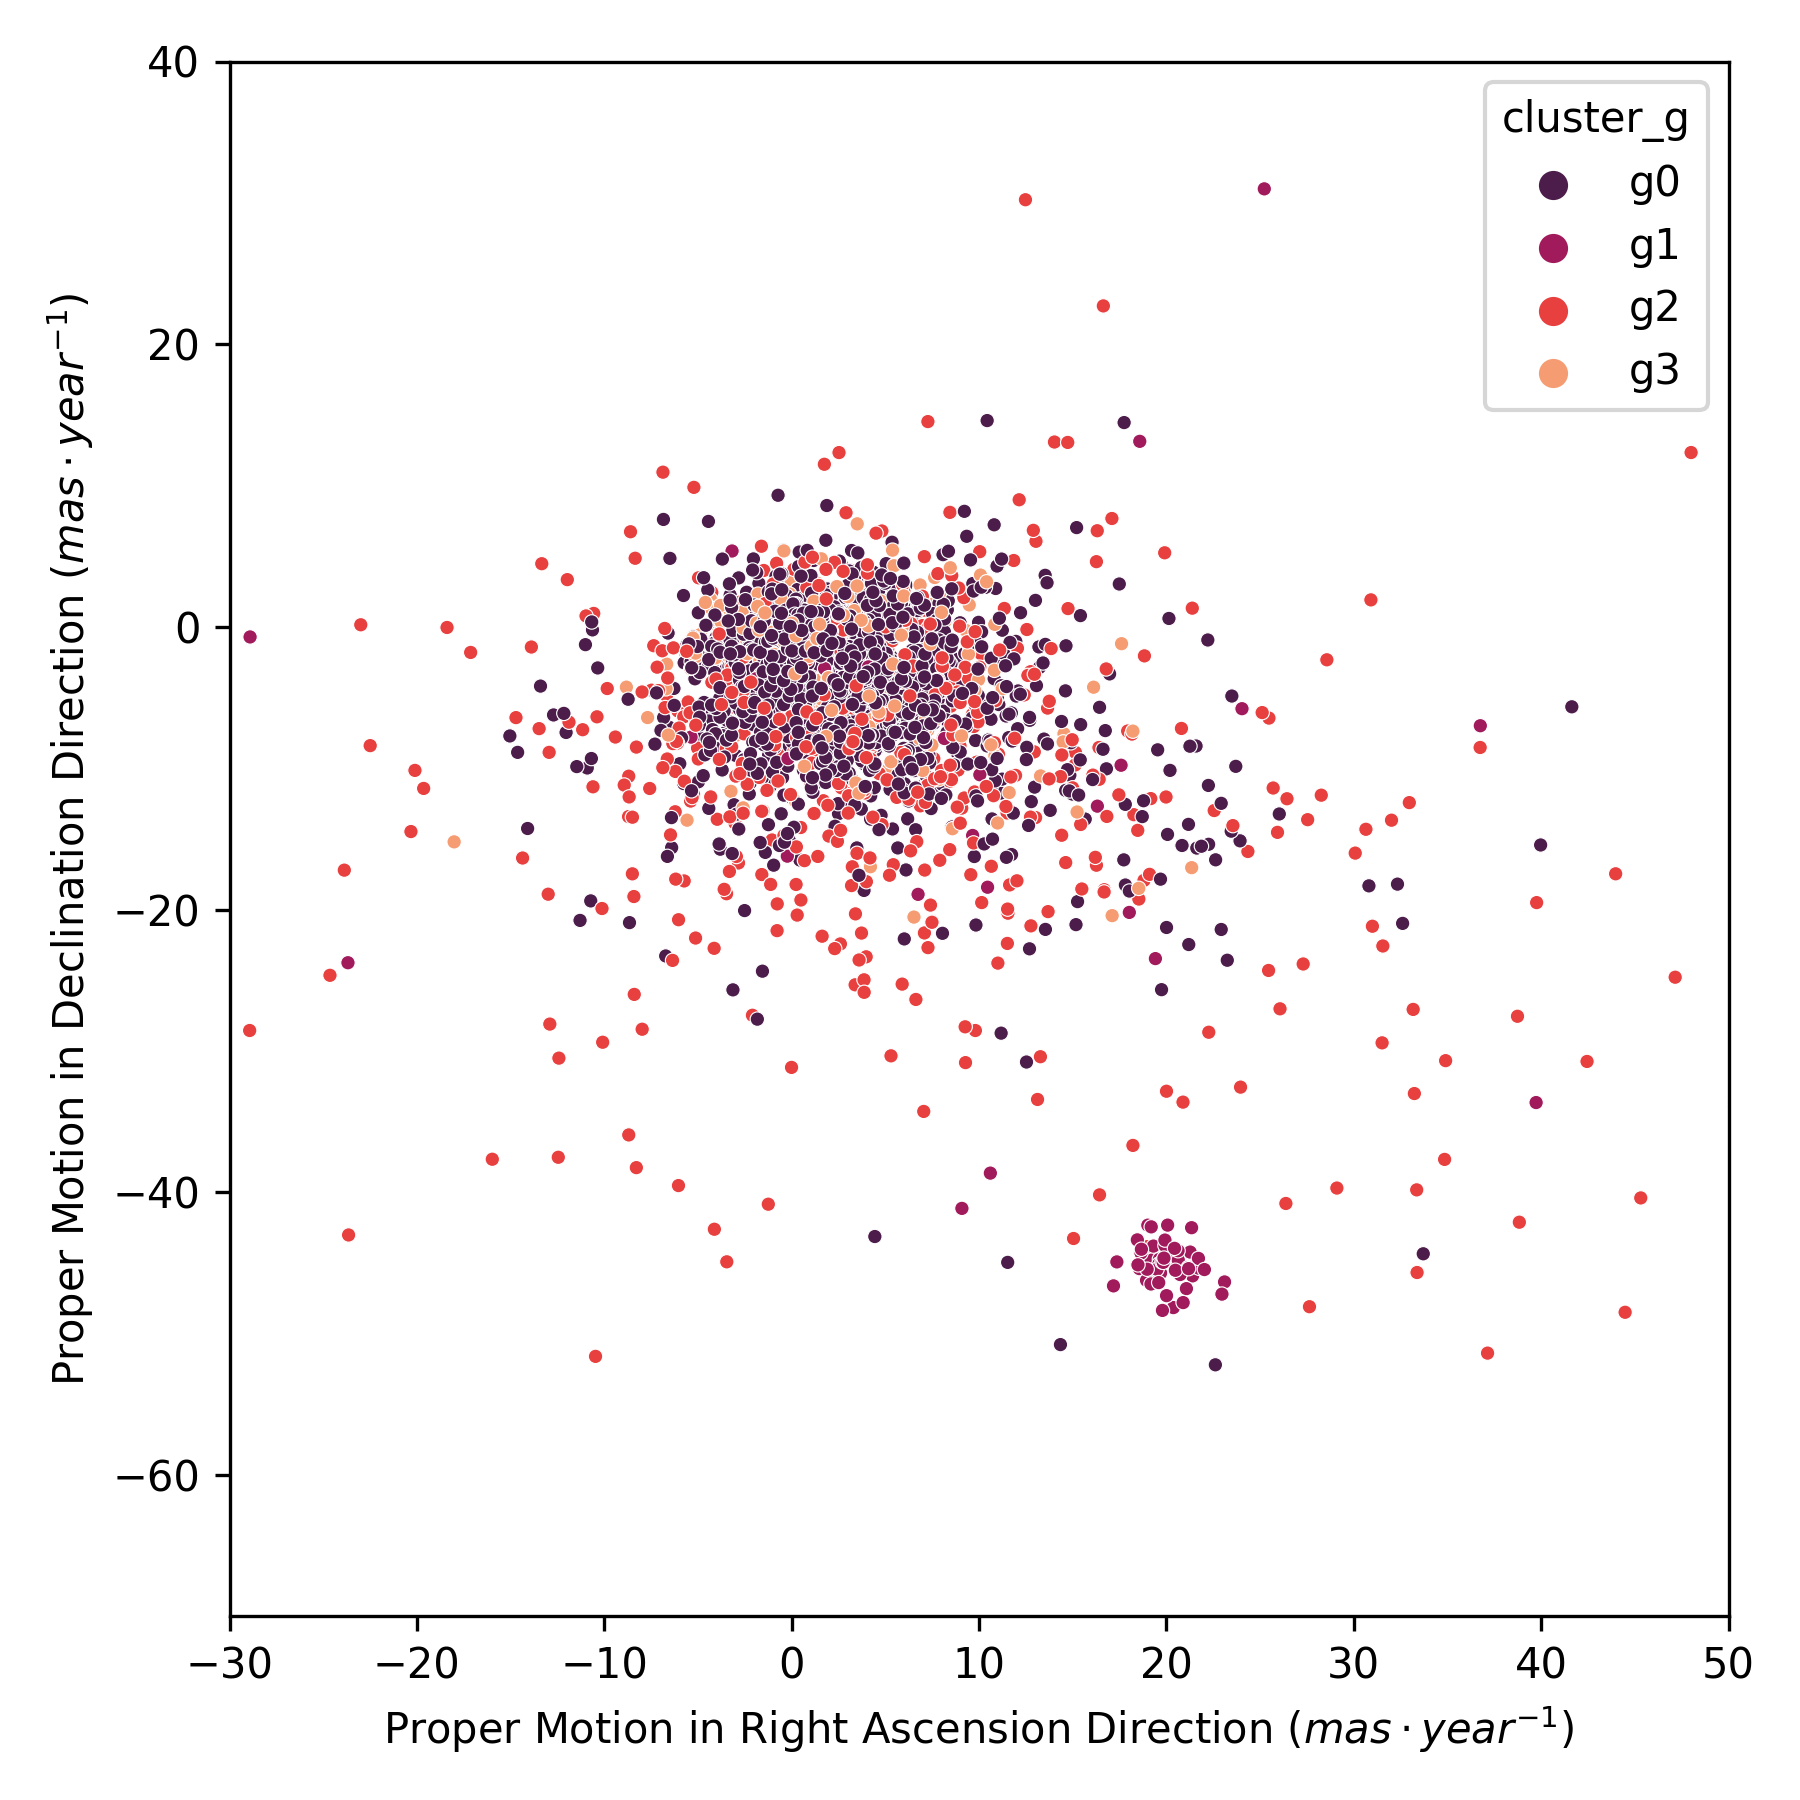
\includegraphics[width=\textwidth]{../figures/kmeans/kmeans_n5_pm_melotte_22.png}
    \end{subfigure}
    \hfill
    \begin{subfigure}[t]{0.3\textwidth}
      \centering
      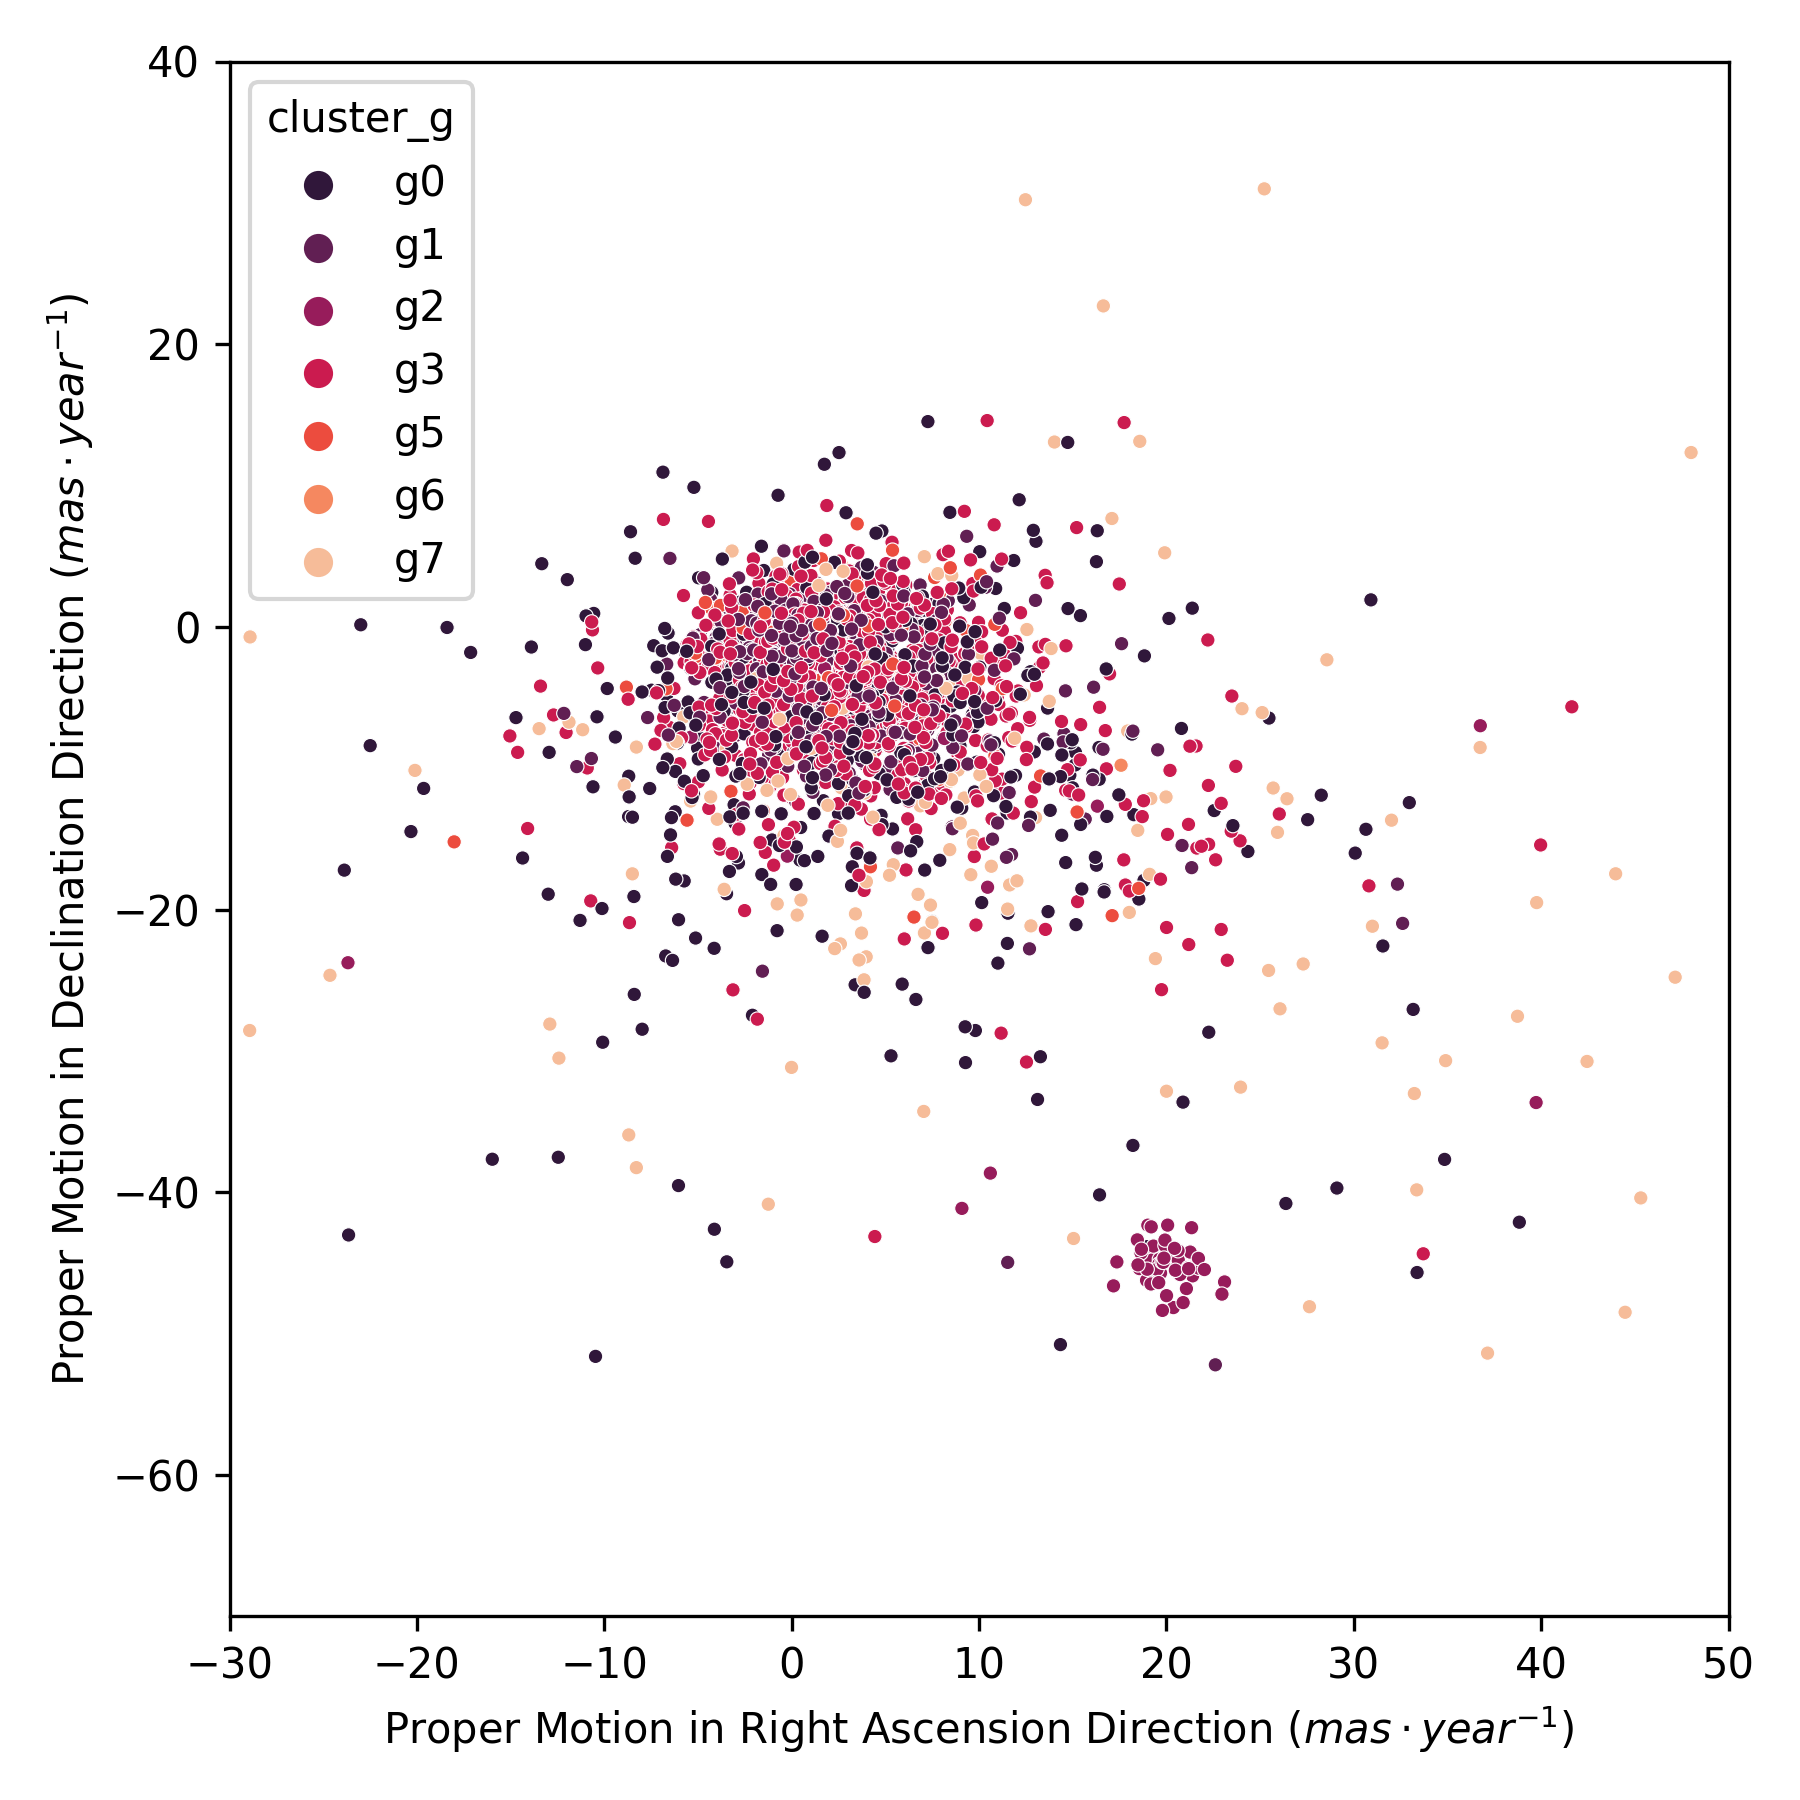
\includegraphics[width=\textwidth]{../figures/kmeans/kmeans_n8_pm_melotte_22.png}
    \end{subfigure}
  \end{subfigure}
  \medskip
  \begin{subfigure}{0.9\textwidth}
    \centering
    \begin{subfigure}[t]{0.3\textwidth}
      \centering
      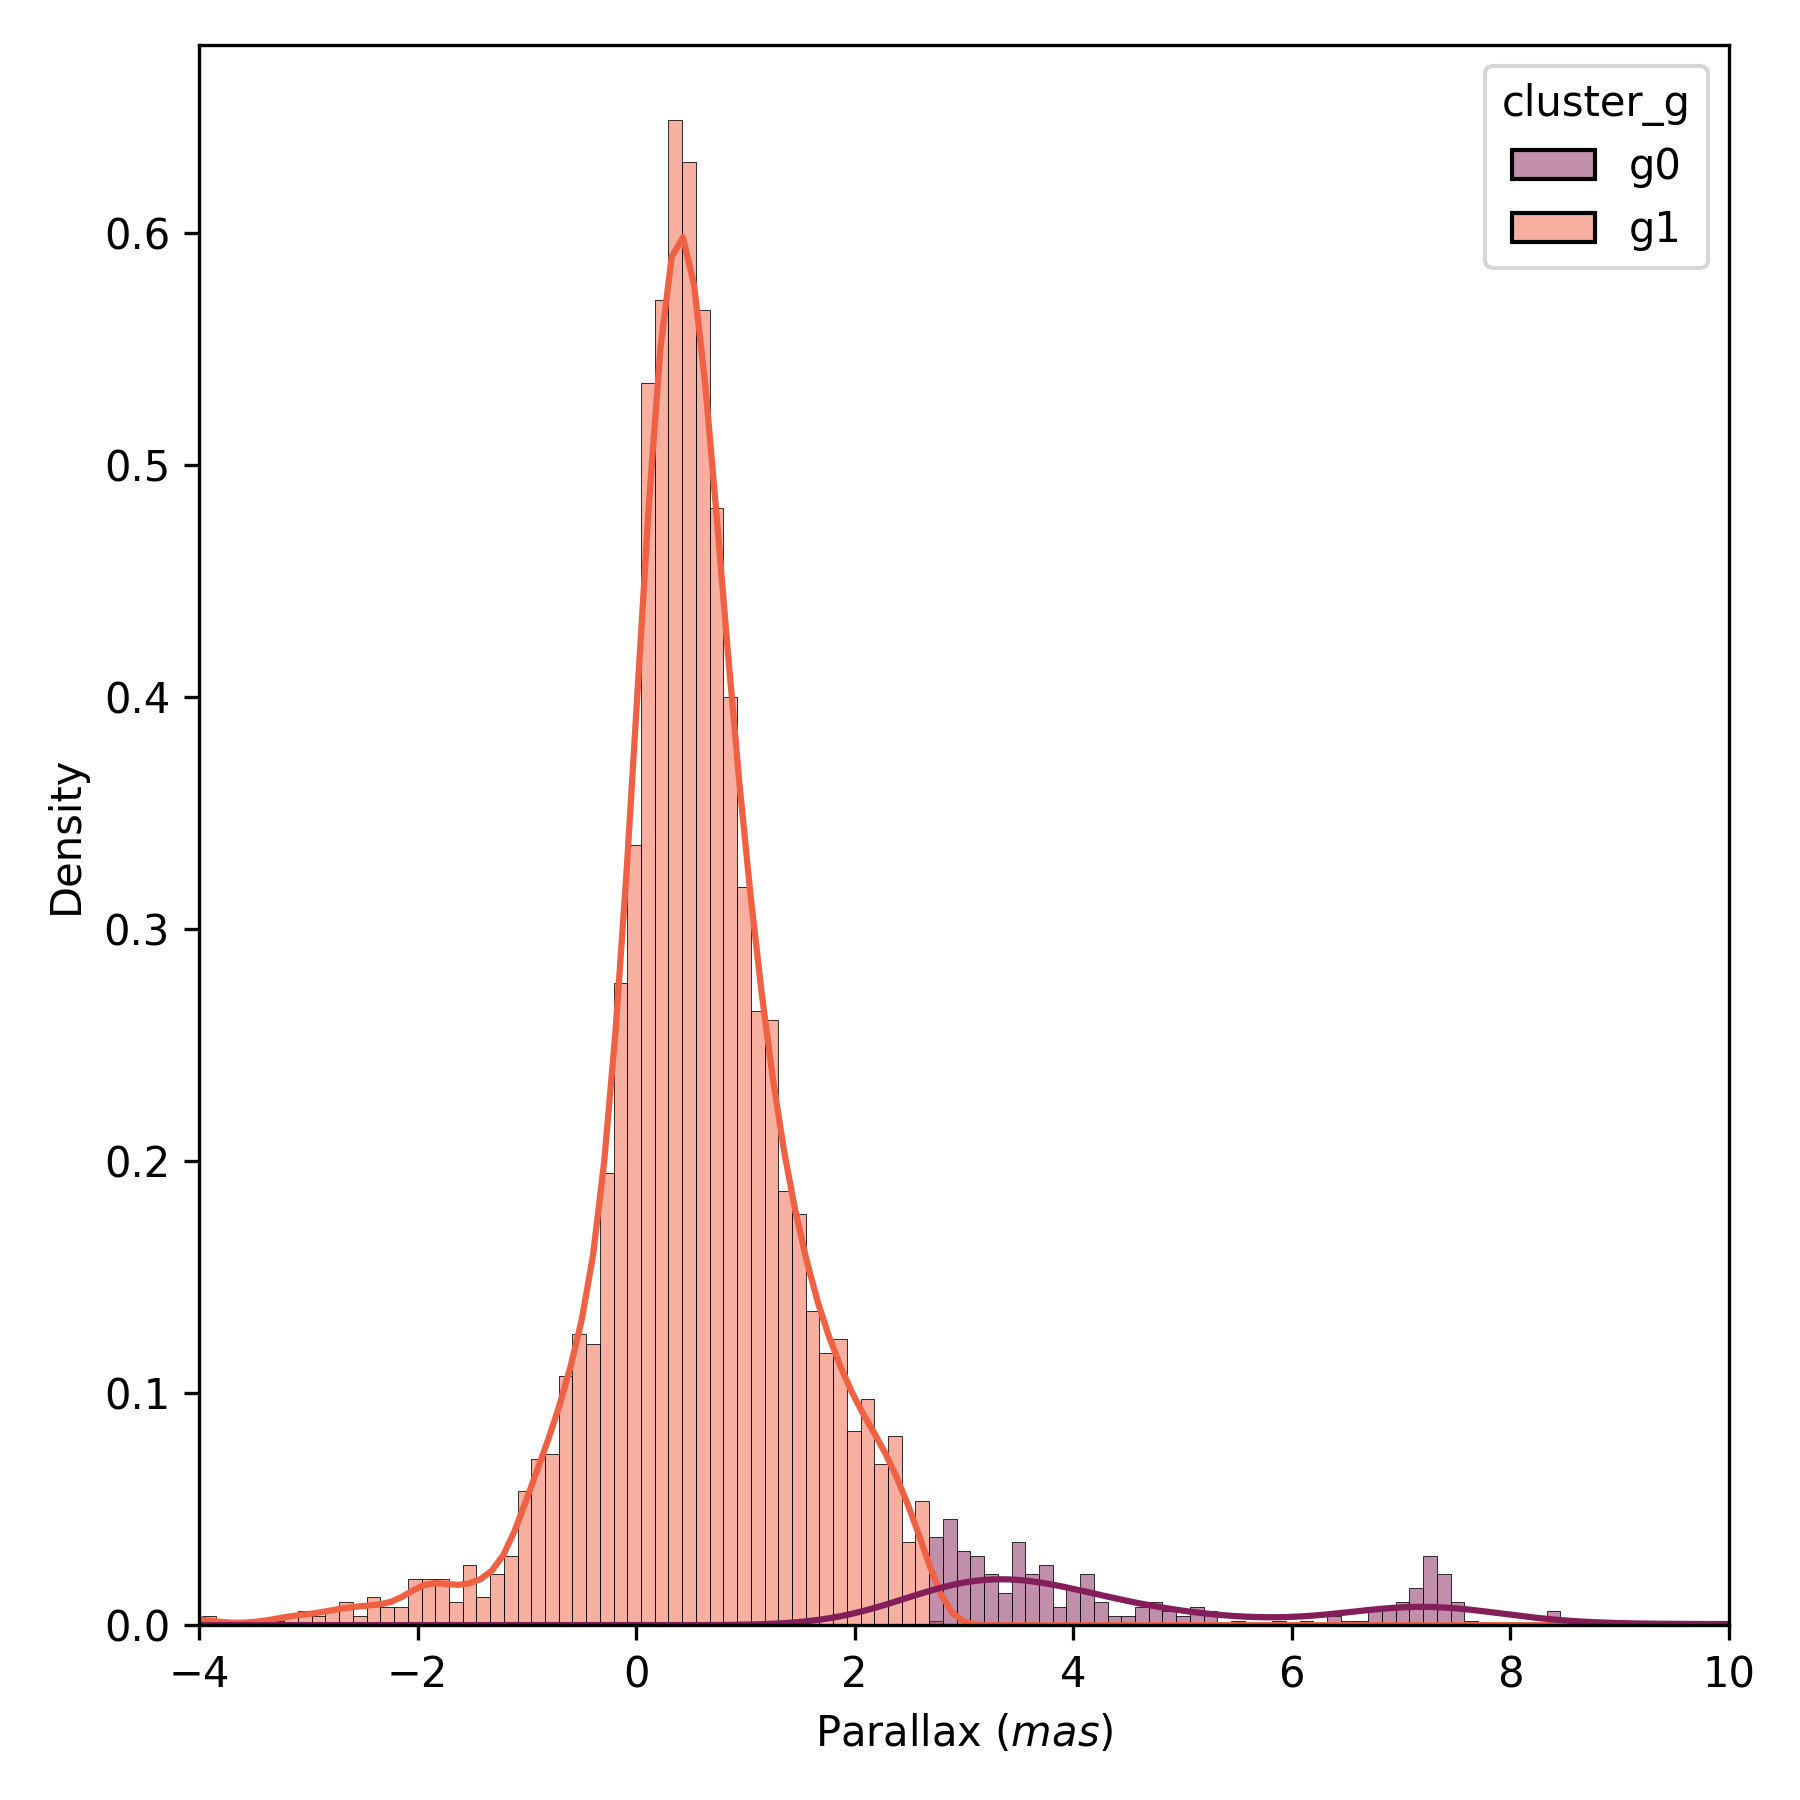
\includegraphics[width=\textwidth]{../figures/kmeans/kmeans_n2_parallax_melotte_22.png}
      \caption{N clusters = 2}
    \end{subfigure}
    \hfill
    \begin{subfigure}[t]{0.3\textwidth}
      \centering
      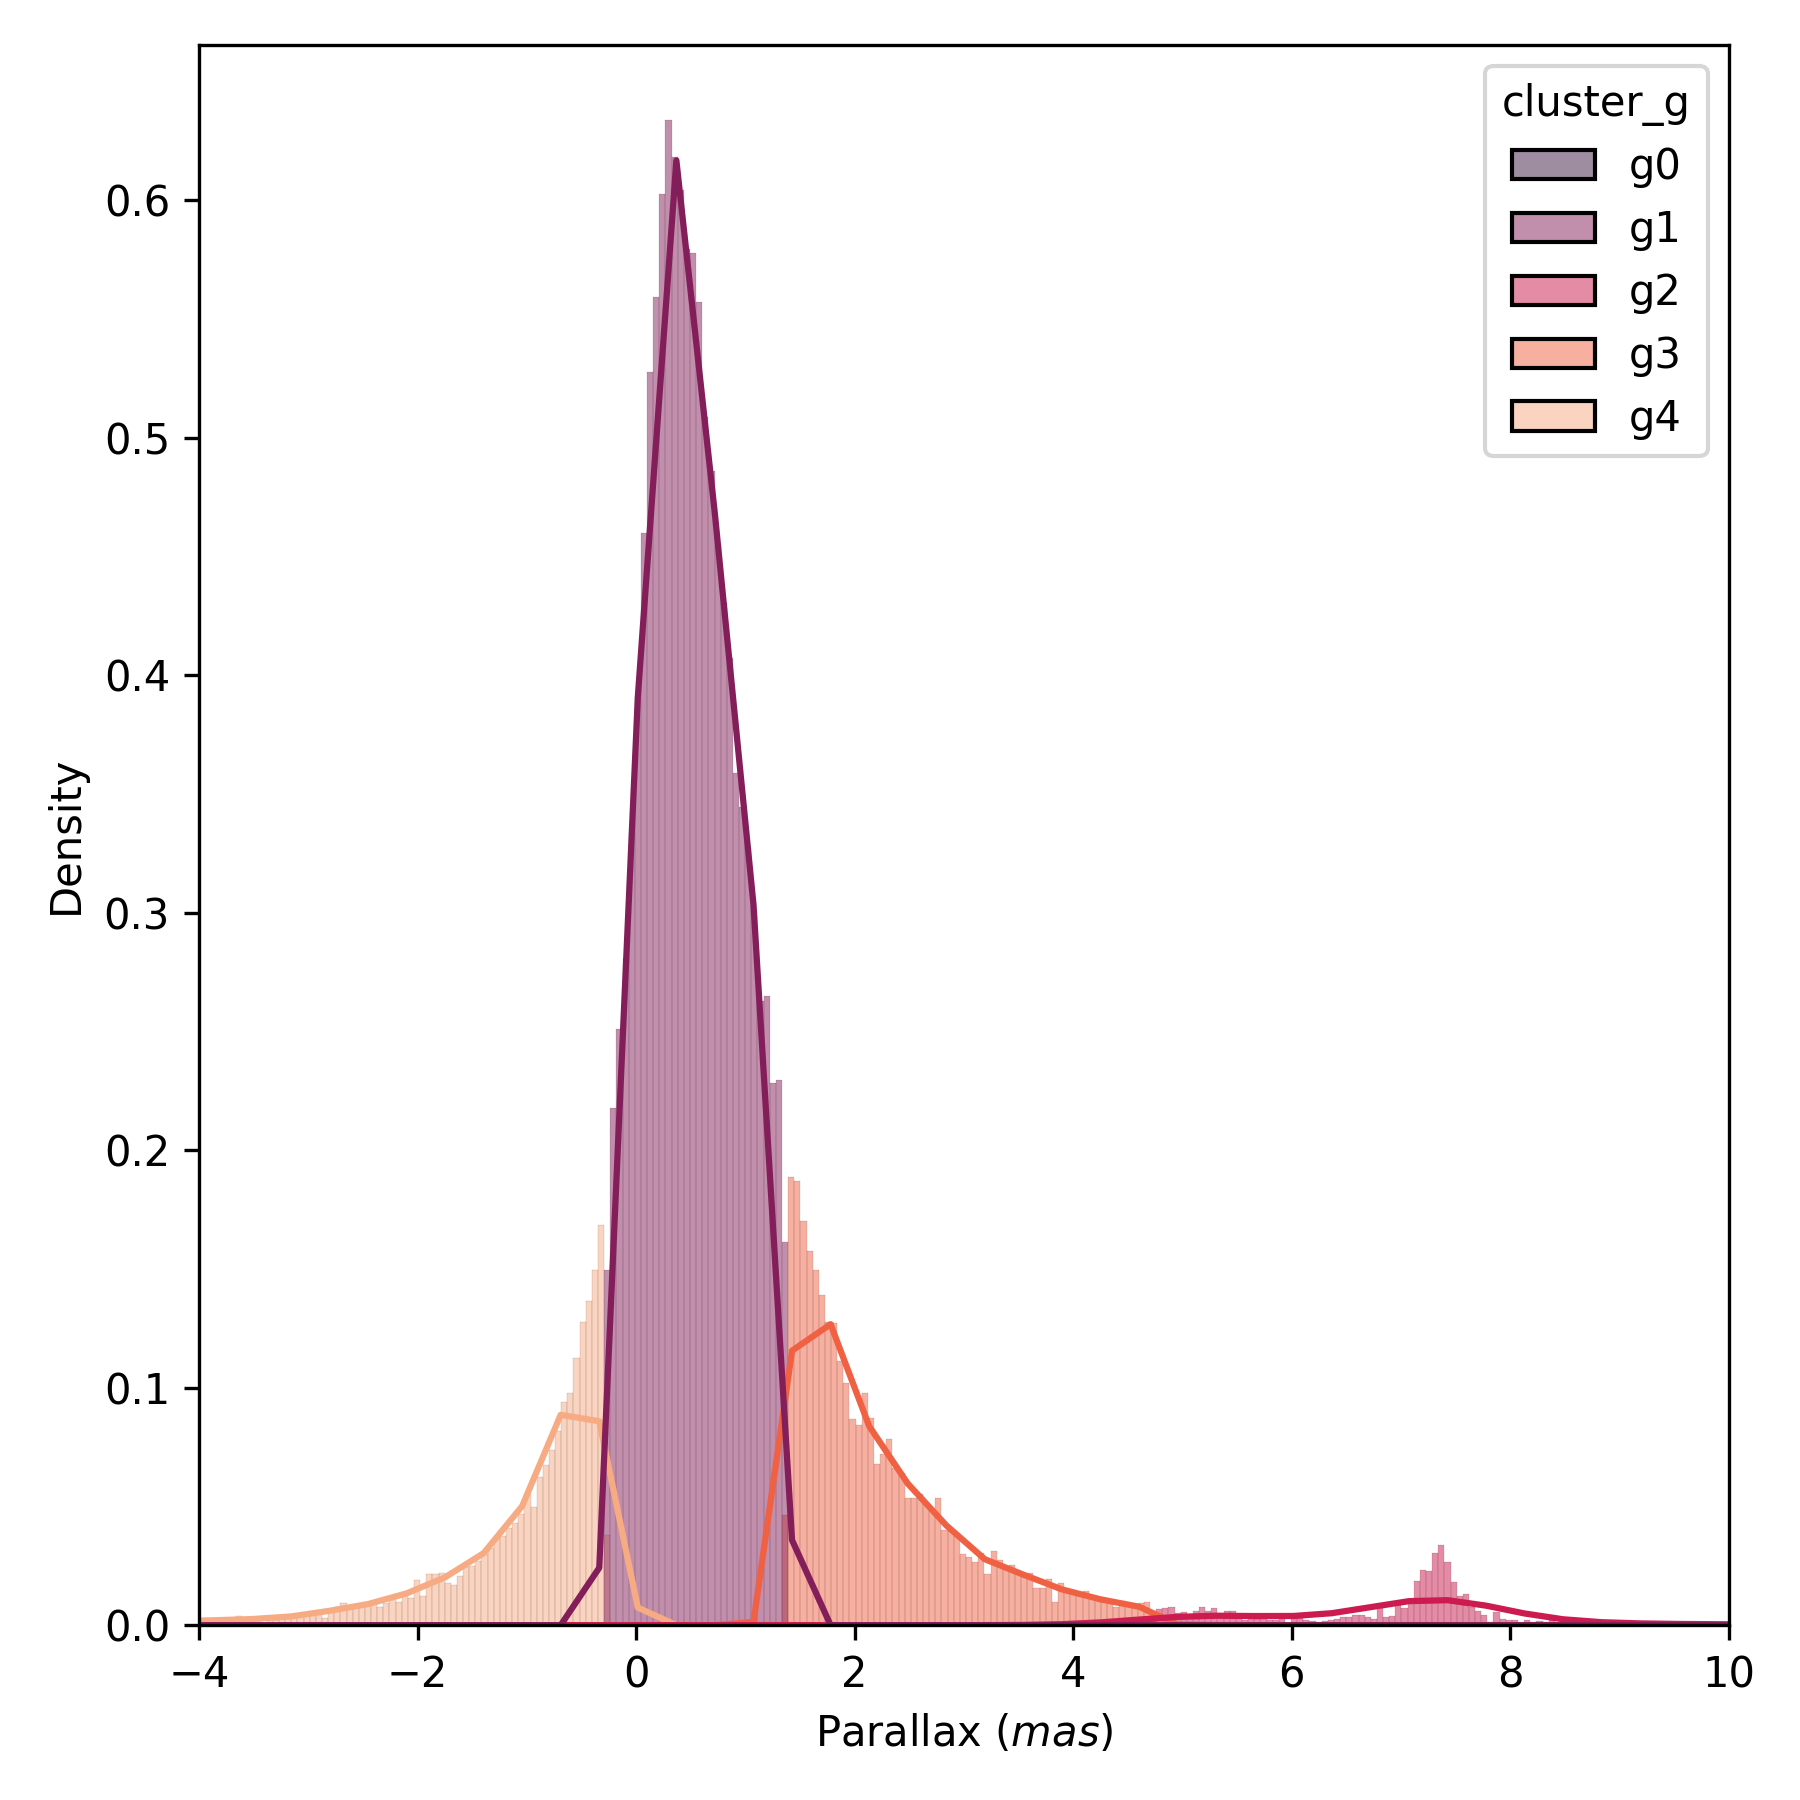
\includegraphics[width=\textwidth]{../figures/kmeans/kmeans_n5_parallax_melotte_22.png}
      \caption{N clusters = 5}
    \end{subfigure}
    \hfill
    \begin{subfigure}[t]{0.3\textwidth}
      \centering
      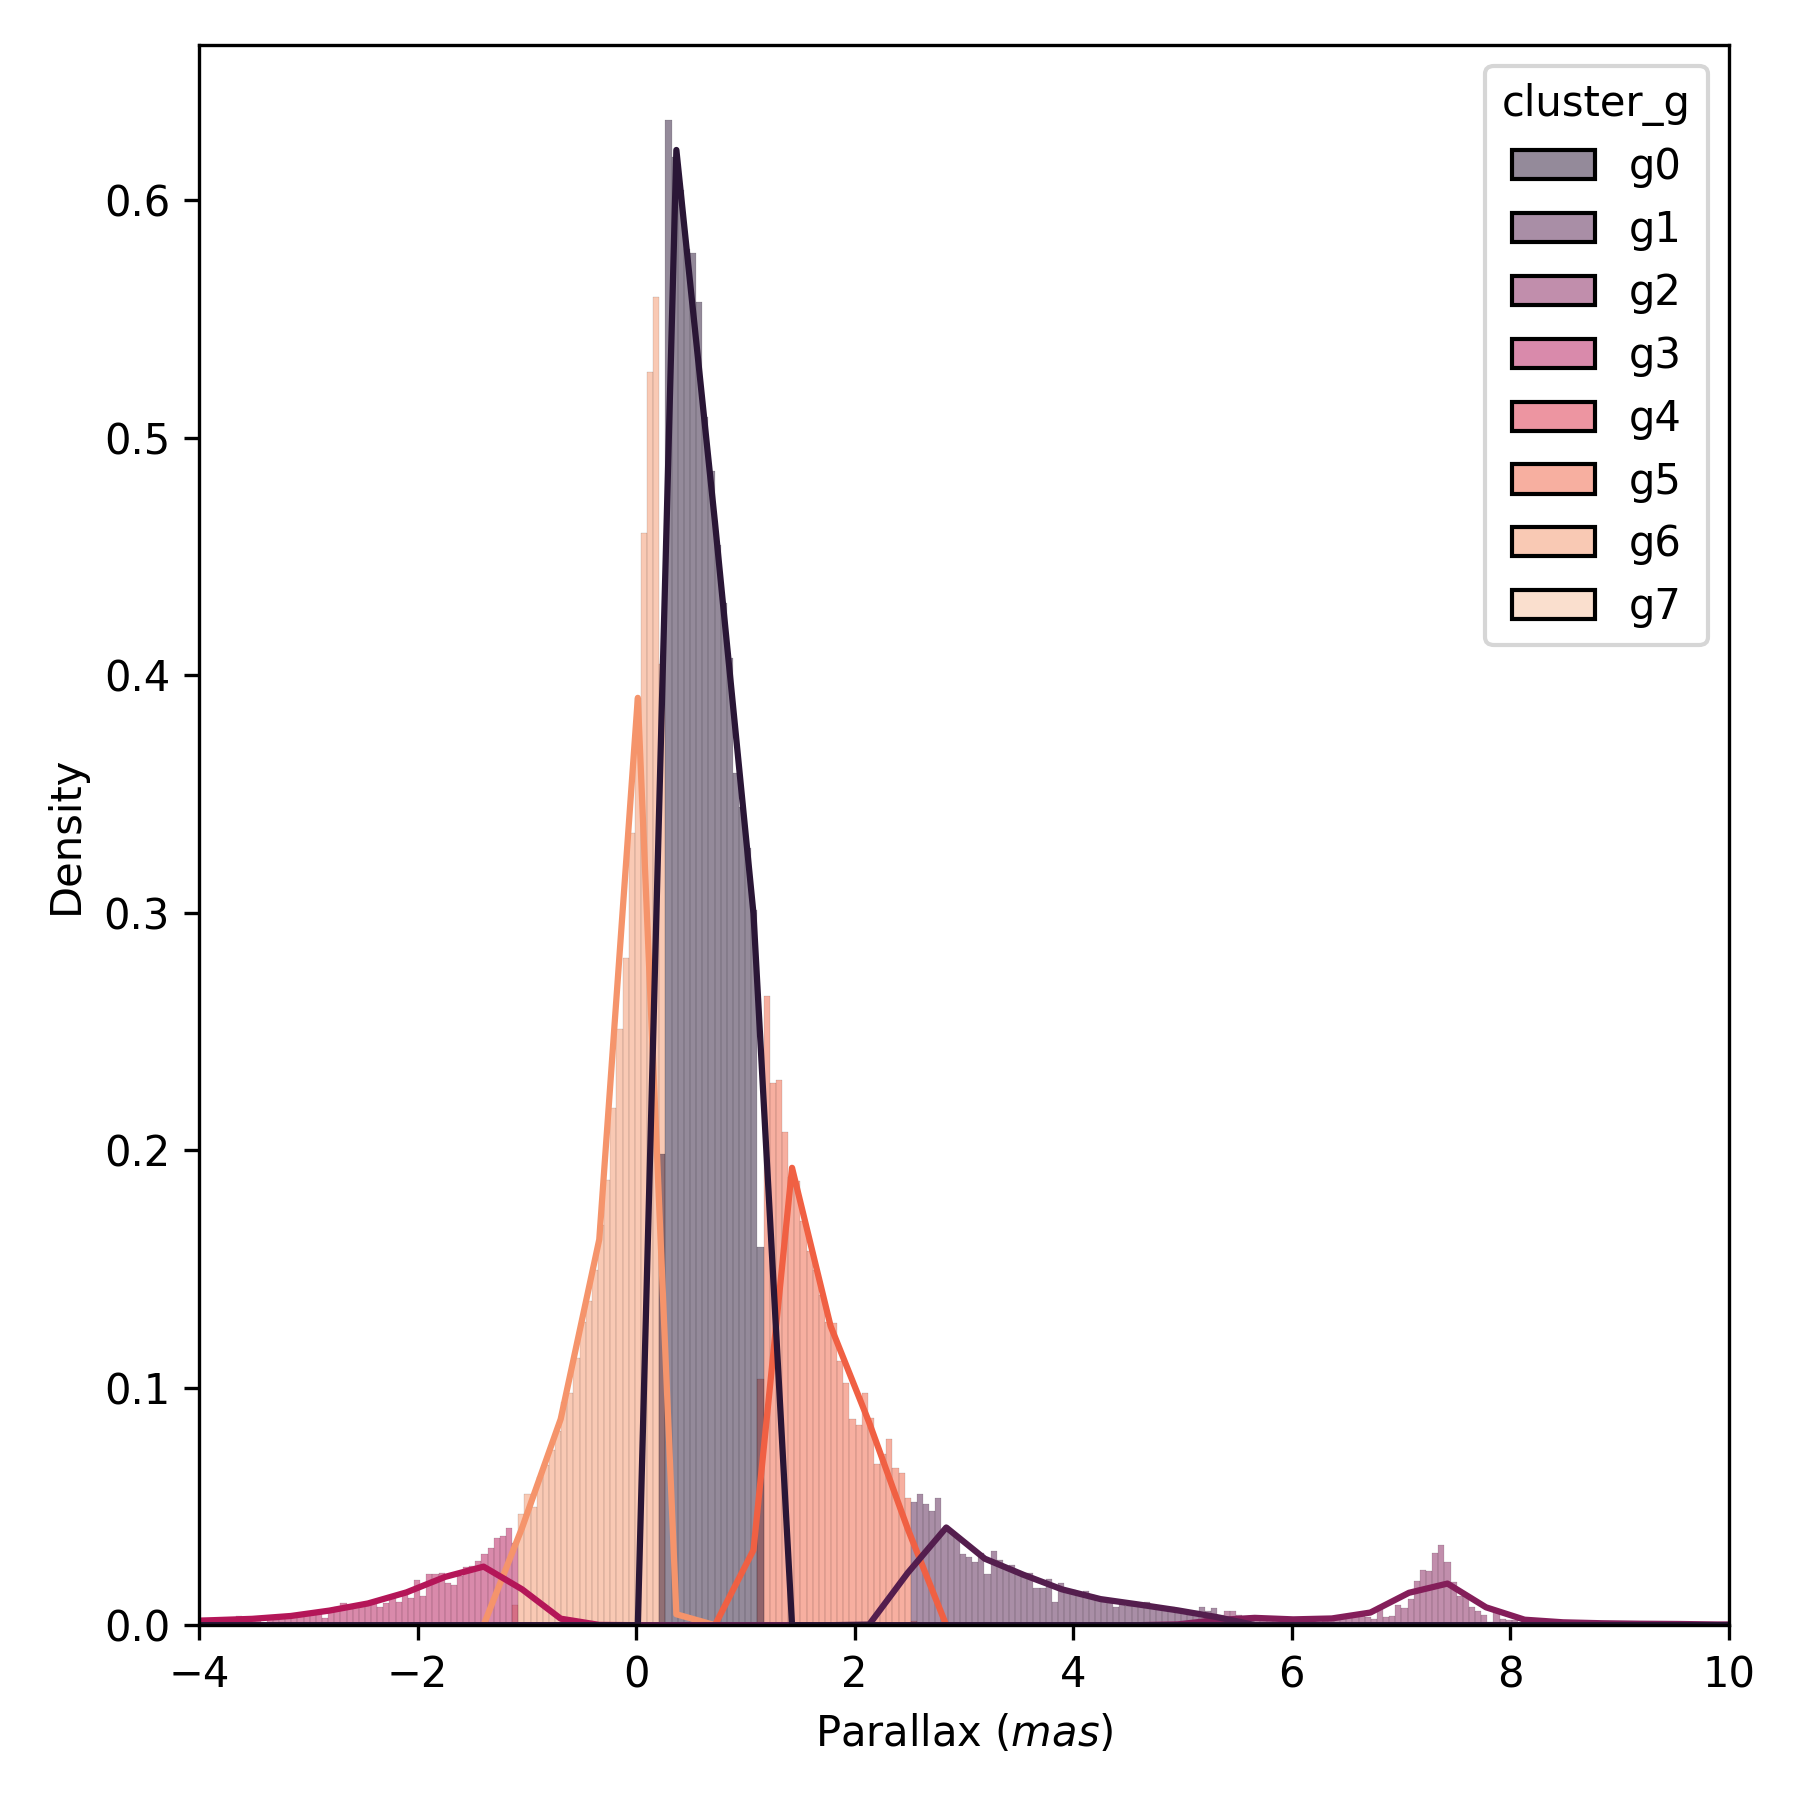
\includegraphics[width=\textwidth]{../figures/kmeans/kmeans_n8_parallax_melotte_22.png}
      \caption{N clusters = 8}
    \end{subfigure}
  \end{subfigure}
  \caption{K-Means comparisons with Melotte 22}
  \label{fig:kmeans_comparisons_melotte_22}
\end{figure}

This is due to the fact that OC's stars are surrounded by other stars with possibly similar properties. So, setting the number of clusters
to two is too low to separate them properly.

As shown in Figure \ref{fig:kmeans_comparisons_melotte_22}, bigger values for the number of clusters allow us to isolate more accurately
the resonance in parallax at $\approx 7.3mas$. However, we have the disadvantage that more groups are formed, while our aim is to find just
one small cluster that contains the stars that belong to the OC and another one with the remaining stars.

This effect complicates our task of finding the desired OC. Therefore, we have to find
a way to set the right value for the number of clusters to isolate the searched cluster without creating too many groups.

To solve this issue, we will try to estimate the best number of clusters by using one more time the \emph{silhouette score}.

The following example can be found in the Jupyter notebook: \verb|cluster_characterization.ipynb| (available at \verb|src/notebooks|).
It shows how to estimate the best number of clusters for Melotte 22 by using \verb|cdalvaro.ml.estimate_n_clusters| method.

\begin{minted}{python}
  n_clusters, kmeans = estimate_n_clusters(melotte22_df, min_clusters=3,
                                           max_clusters=10, verbose=True)

  # Output
  # Silhouette score for 3 clusters: 0.5420
  # Silhouette score for 4 clusters: 0.5393
  # Silhouette score for 5 clusters: 0.5608
  # Silhouette score for 6 clusters: 0.5336
  # Silhouette score for 7 clusters: 0.5306
  # Silhouette score for 8 clusters: 0.4978
  # Silhouette score for 9 clusters: 0.5214
  # Silhouette score for 10 clusters: 0.5199
  # Best silhouette score is 0.5608 for 5 clusters
\end{minted}

K-Means does a good job making an initial clustering, as shown in Figure \ref{fig:kmeans_melotte_22}. However, too many clusters arise from this characterization
and the open cluster is still polluted with stars that do not belong to it. Even more, we would like to reduce the amount of clusters too.

\begin{figure}[htbp]
  \centering
  \begin{subfigure}{0.9\textwidth}
    \centering
    \begin{subfigure}[t]{.45\textwidth}
      \centering
      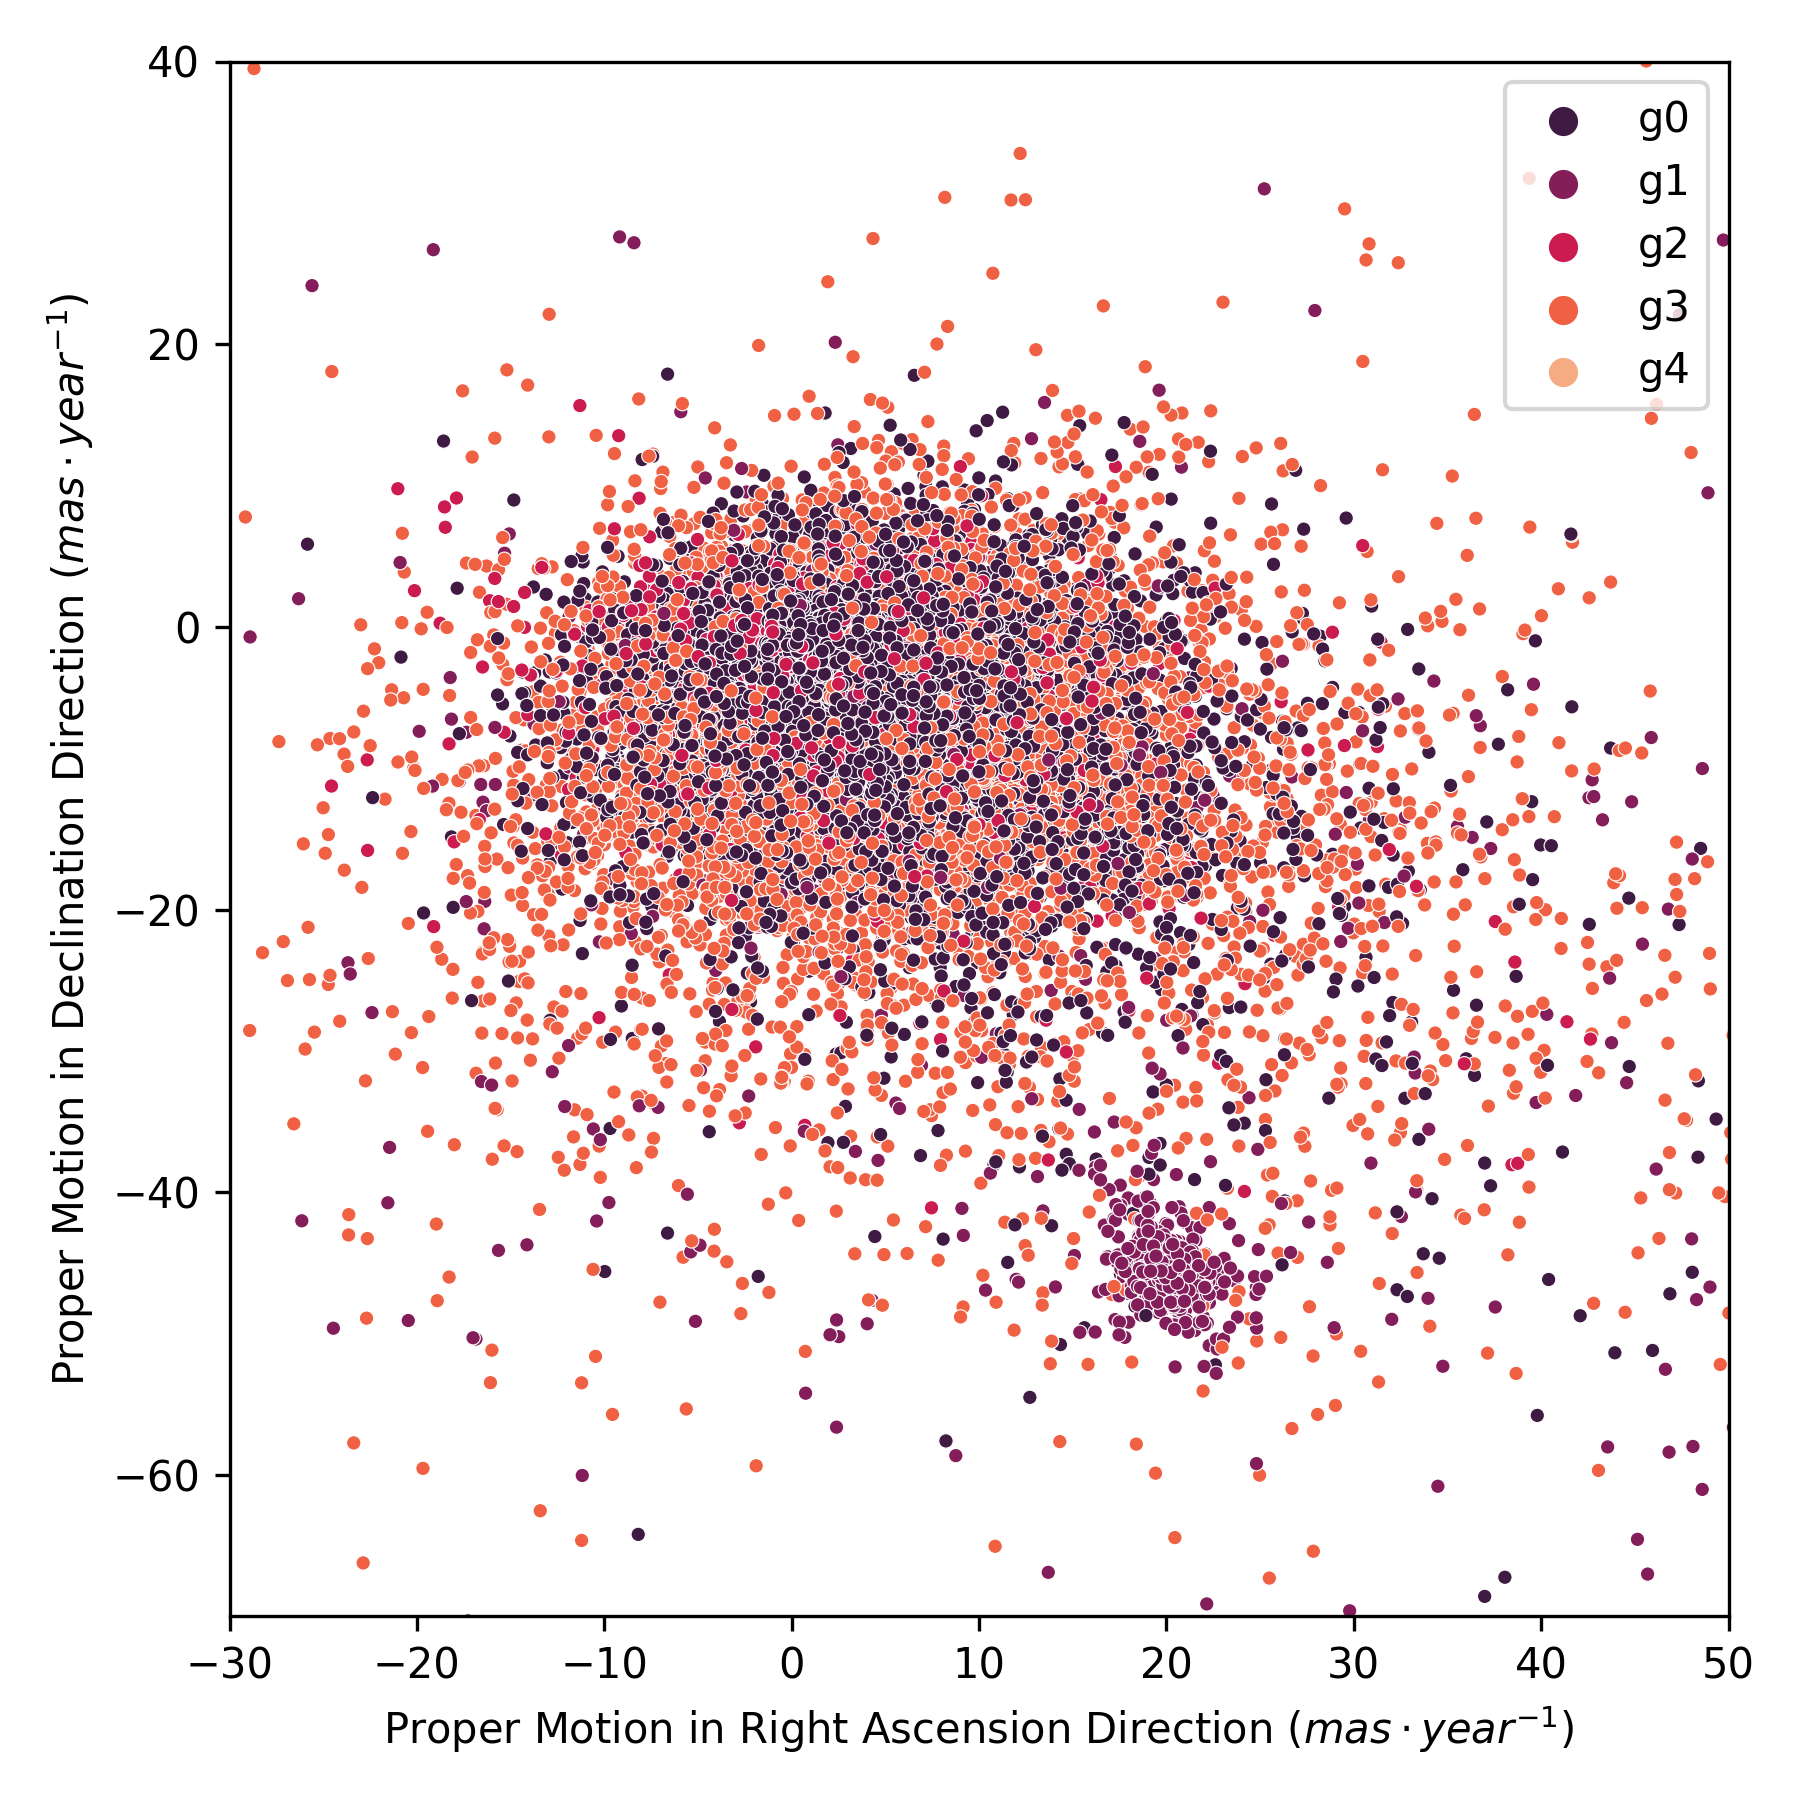
\includegraphics[width=\textwidth]{../figures/melotte_22/kmeans_pm_melotte_22.png}
      \caption{Proper Motion}
    \end{subfigure}
    \hfill
    \begin{subfigure}[t]{.45\textwidth}
      \centering
      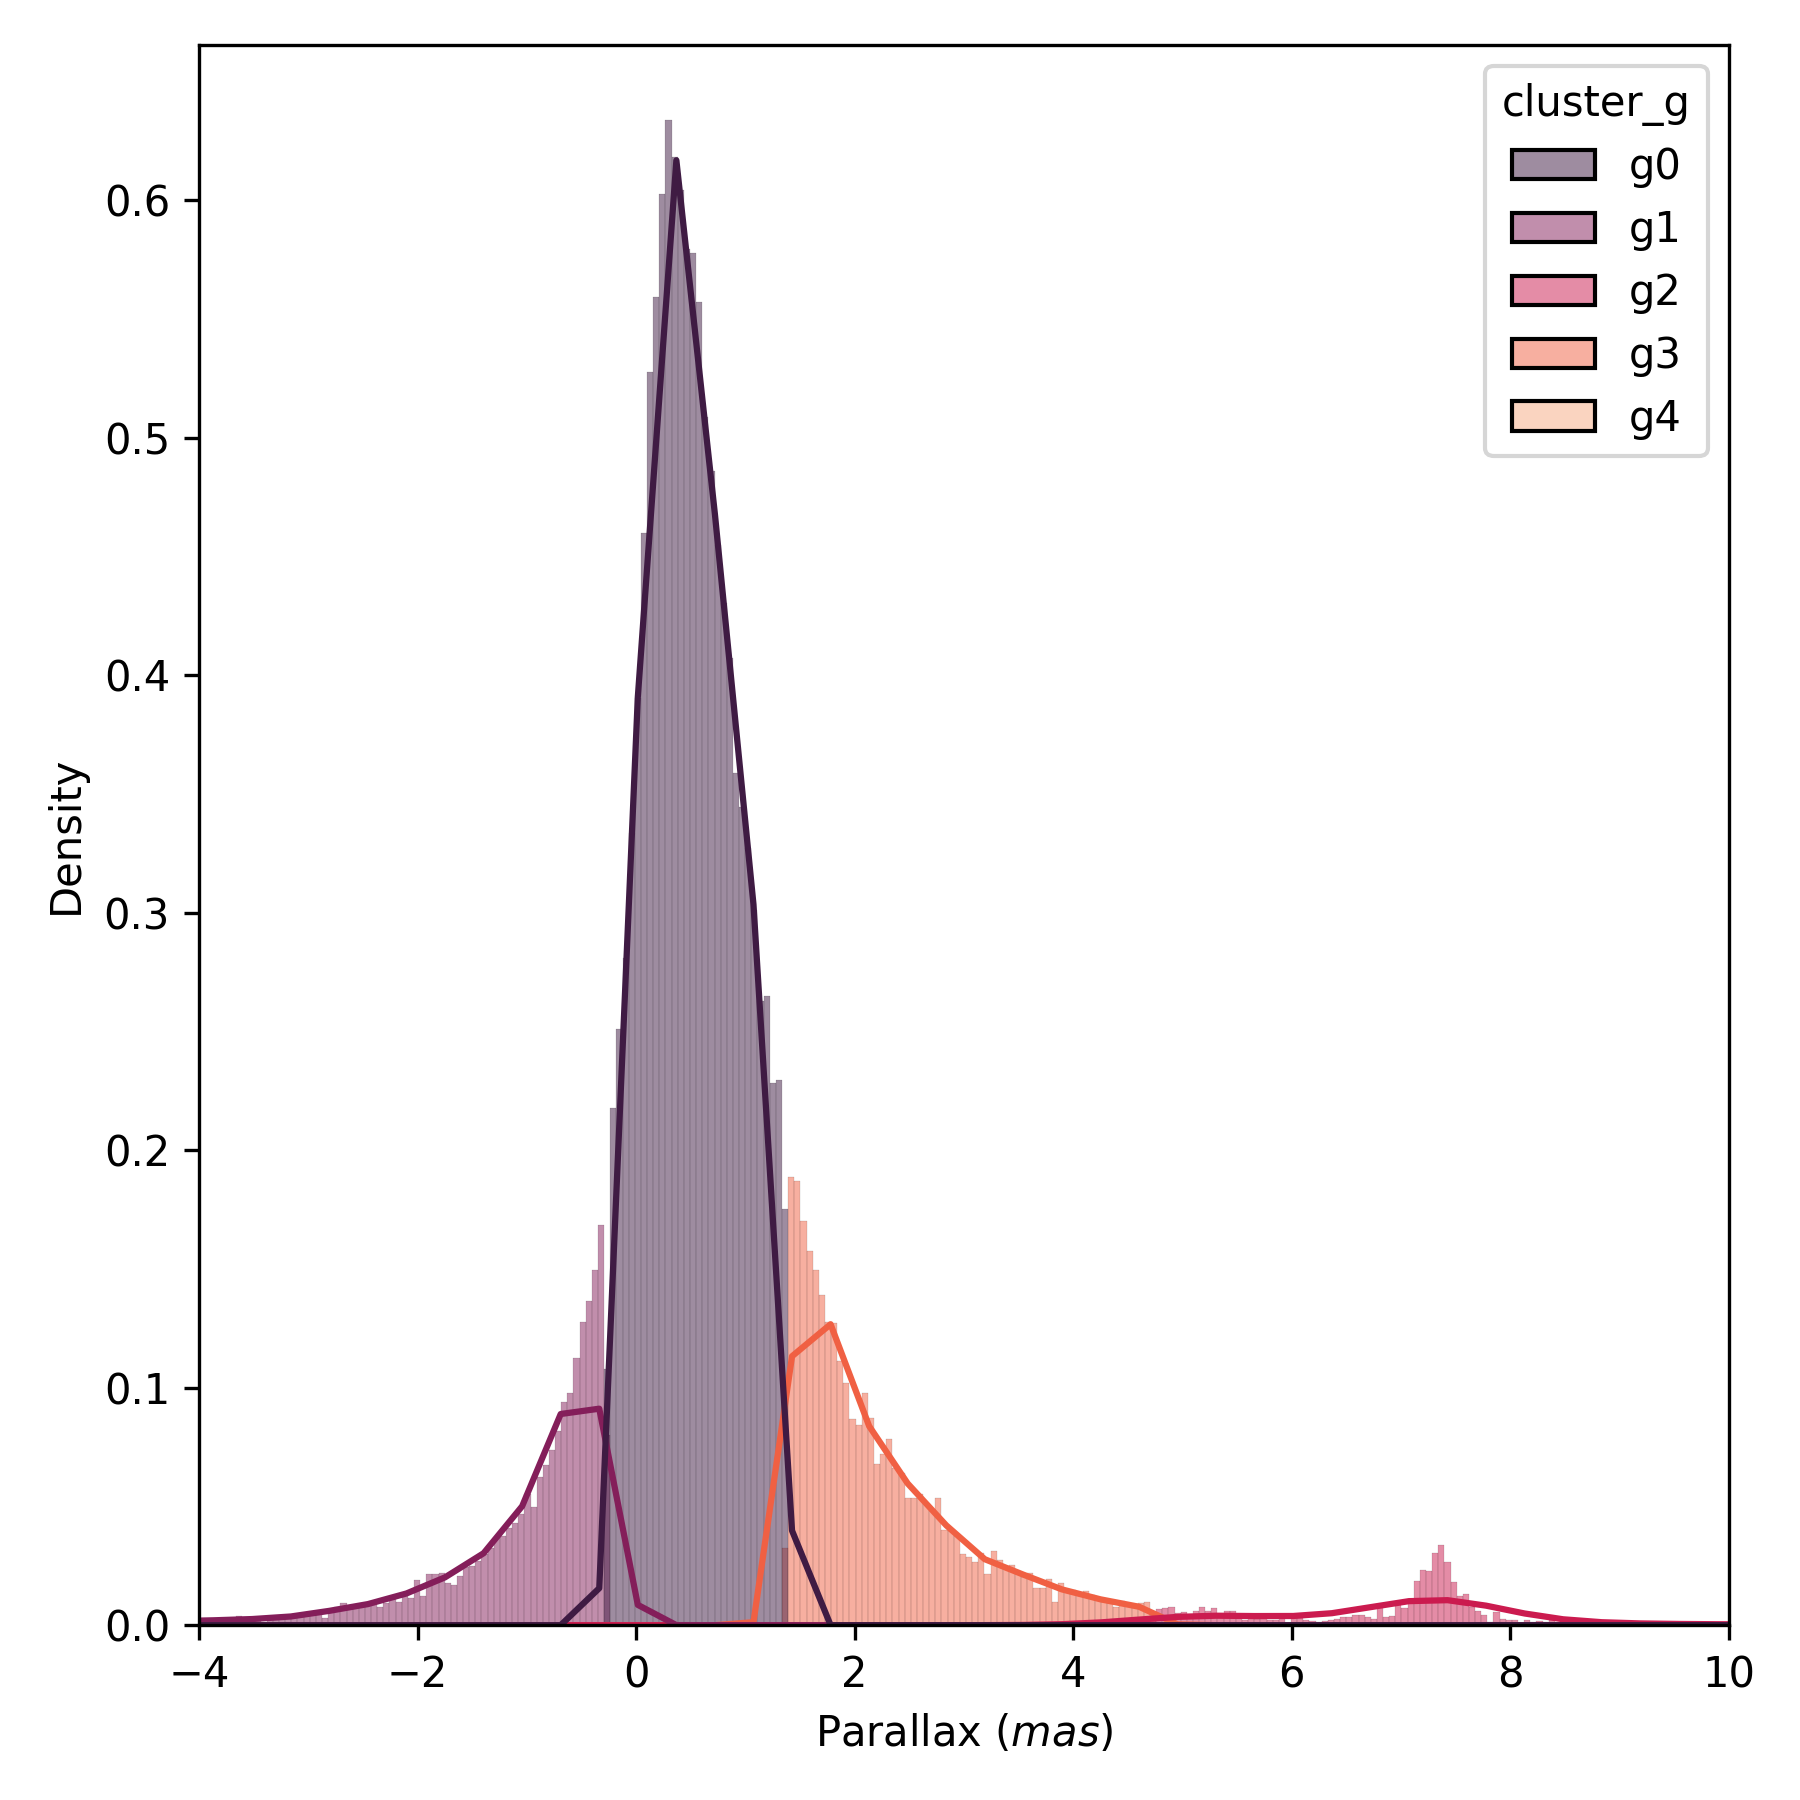
\includegraphics[width=\textwidth]{../figures/melotte_22/kmeans_parallax_melotte_22.png}
      \caption{Parallax}
    \end{subfigure}
  \end{subfigure}
  \caption{K-Means model applied to Melotte 22}
  \label{fig:kmeans_melotte_22}
\end{figure}

If we take a look into the H-R diagram (Figure \ref{fig:kmeans_hr_diagram_melotte_22}), we can identify the isochrone curve for Melotte 22 cluster.
This curve has a good shape, but again, it contains outsider stars. Therefore, we would like to find a better model that improves this initial characterization
by reducing the amount of clusters and also that would be able to remove outsiders from the OC.

\begin{figure}[htbp]
  \centering
  \begin{subfigure}{0.5\textwidth}
    \centering
    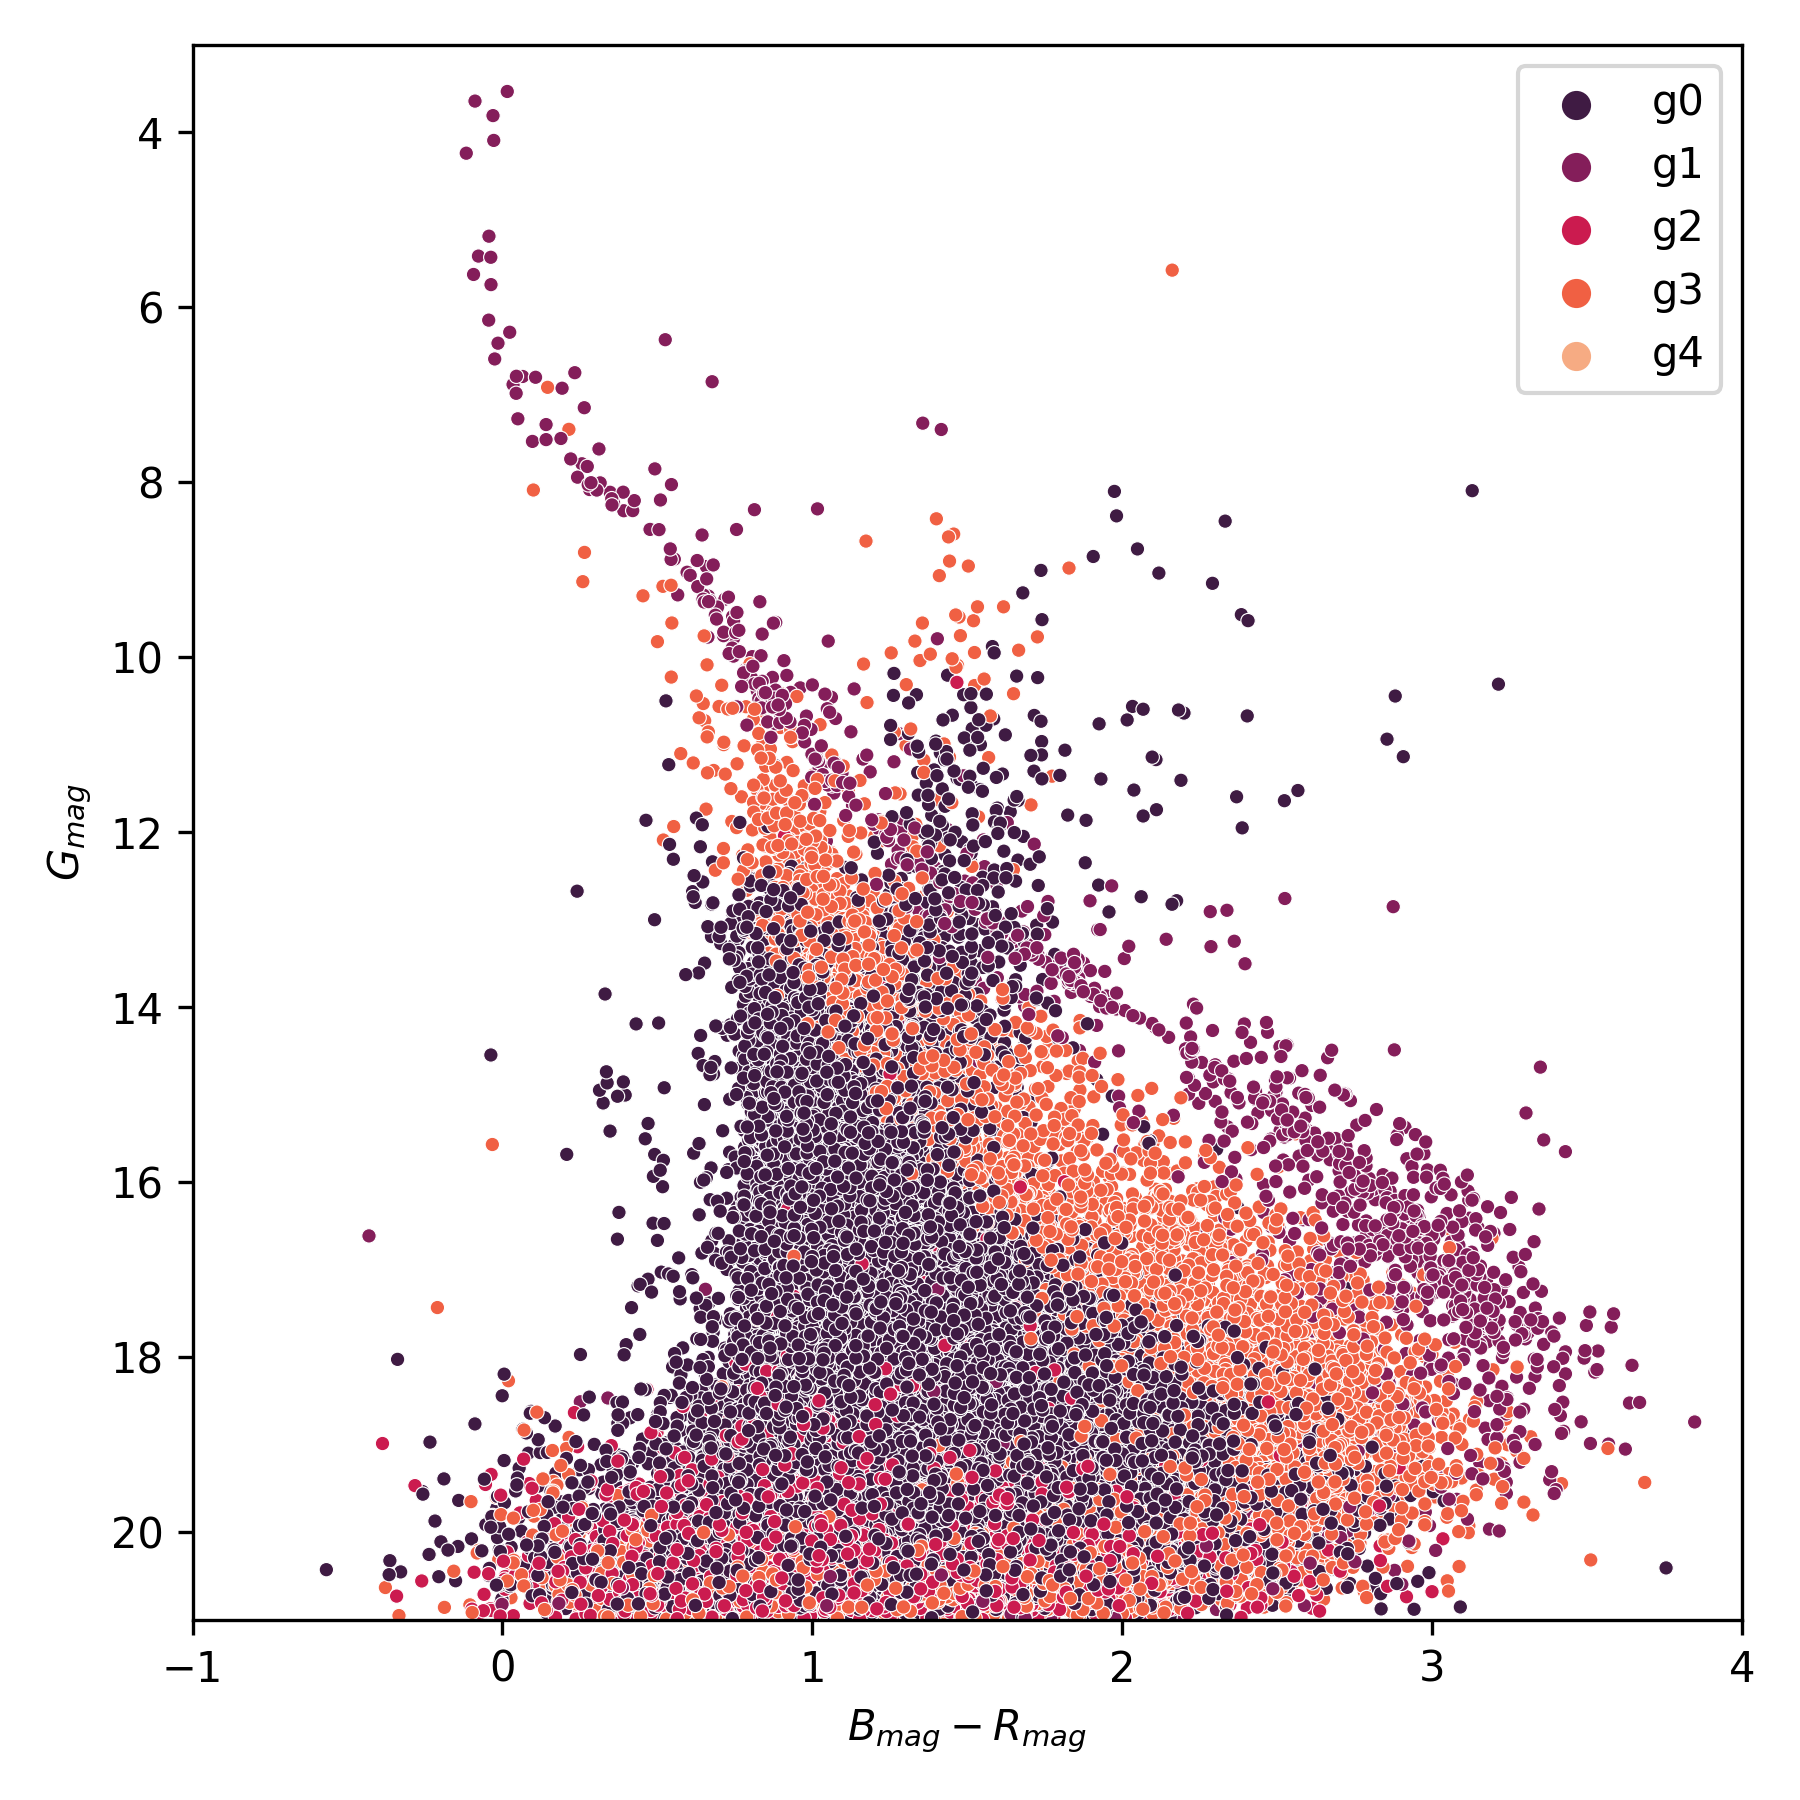
\includegraphics[width=\textwidth]{../figures/melotte_22/kmeans_hr_diagram_melotte_22.png}
  \end{subfigure}
  \caption{Melotte 22 H-R diagram with K-Means characterization}
  \label{fig:kmeans_hr_diagram_melotte_22}
\end{figure}

\section{Deep Embedded Clustering (DEC)}

Our initial approach allows us to find some groups that potentially contain the desired OC. However, as we have seen, the result is not enough
accurate. Therefore, we need a method for merging clusters by migrating stars from one group to another,
so we can end up with the minimum number of clusters while preserving the open cluster.

Since we do not have a labeled dataset which allows us to train a supervised model, we have no choice but to use an unsupervised self-trained model.

For that reason we have adapted the \emph{Unsupervised Deep Embedding for Clustering Analysis} or \emph{DEC} model \cite{xie2016unsupervised} to our work.

The implementation of this model is available in \verb|cdalvaro.ml.DEC| and it is developed with the Keras framework.

The model is composed by a \emph{deep autoencoder}, a \emph{deep encoder} and a \emph{clustering layer}.

Encoders are used to transform the input data into a latent space using a non-linear mapping function $f_{\theta} : X \rightarrow Z$.

Although, as explained in section \ref{sec:feature_selection}, the number of features we are managing is not too large, this latent space allows us to reduce
the number of features, avoiding this way the \emph{"curse of dimensionality"} \cite{bellman1961curse}.

These encoders are pretrained before fitting the model to generate predictions. Then, the encoder is used to transform input data to the
latent space $Z$. Once the data has been transformed, a K-Means clusterer is used to make an initial clustering.

With that initial configuration, the model iterates alternating between computing an auxiliary target distribution (Soft Assignment)
and minimizing the Kullback-Leiber (KL) divergence \cite{kullback1951information} to it. This unsupervised algorithm allows us to improve
the clustering.

\begin{equation}
  p_{ij} = \frac{q^{2}_{ij} / f_{j}}{\sum_{j'}q^{2}_{ij'}/f_{j'}}
  \label{eq:student_tdistribution}
\end{equation}

In the soft assignment stage, the \emph{Student's t-distribution} is used as a kernel to measure the similarity
between the embedded points and the cluster centroid. While in the KL divergence minimization the algorithm iteratively refines clusters by learning
from their high confidence assignments with the help of an auxiliary target distribution. The model is trained by matching the soft assignment to the
target distribution. The choice of this target distribution is crucial for DEC's performance. In this work we have taken the target distribution
from DEC's original paper \cite{xie2016unsupervised}, which is defined in Equation \ref{eq:student_tdistribution}.

Figure \ref{fig:dec_model_setup} shows the layer setup of our DEC model. It is simpler than the one tested on the original paper \cite{xie2016unsupervised},
since the number of selected features in our work is smaller. Therefore, using the same configuration would result in a model too
powerful that would incur in overfitting issues unable to make right predictions.

\begin{figure}[htbp]
  \centering
  \begin{subfigure}{0.9\textwidth}
    \centering
    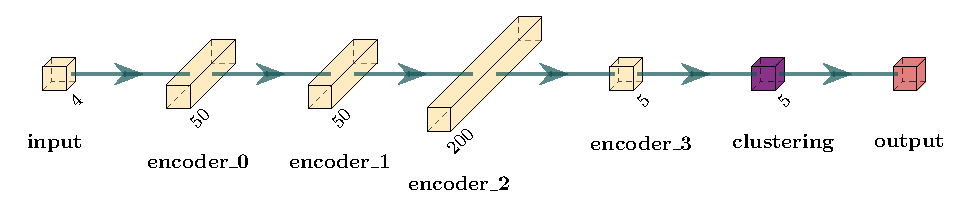
\includegraphics[width=\textwidth]{../figures/dec_diagram.pdf}
  \end{subfigure}
  \caption{DEC model layer setup}
  \label{fig:dec_model_setup}
\end{figure}

Once the model is ready, we can test it by applying it to the Melotte 22 dataset. Notebook \verb|cluster_characterization.ipynb| illustrates how DEC model
processes a region of stars trying to characterize the open cluster hidden within that region.

As shown in Figure \ref{fig:dec_melotte_22}, the DEC model is able to move stars from one group to another removing some clusters and improving the OC characterization.
This is exactly what we are looking for.

\begin{figure}[htbp]
  \centering
  \begin{subfigure}{0.9\textwidth}
    \centering
    \begin{subfigure}[t]{0.45\textwidth}
      \centering
      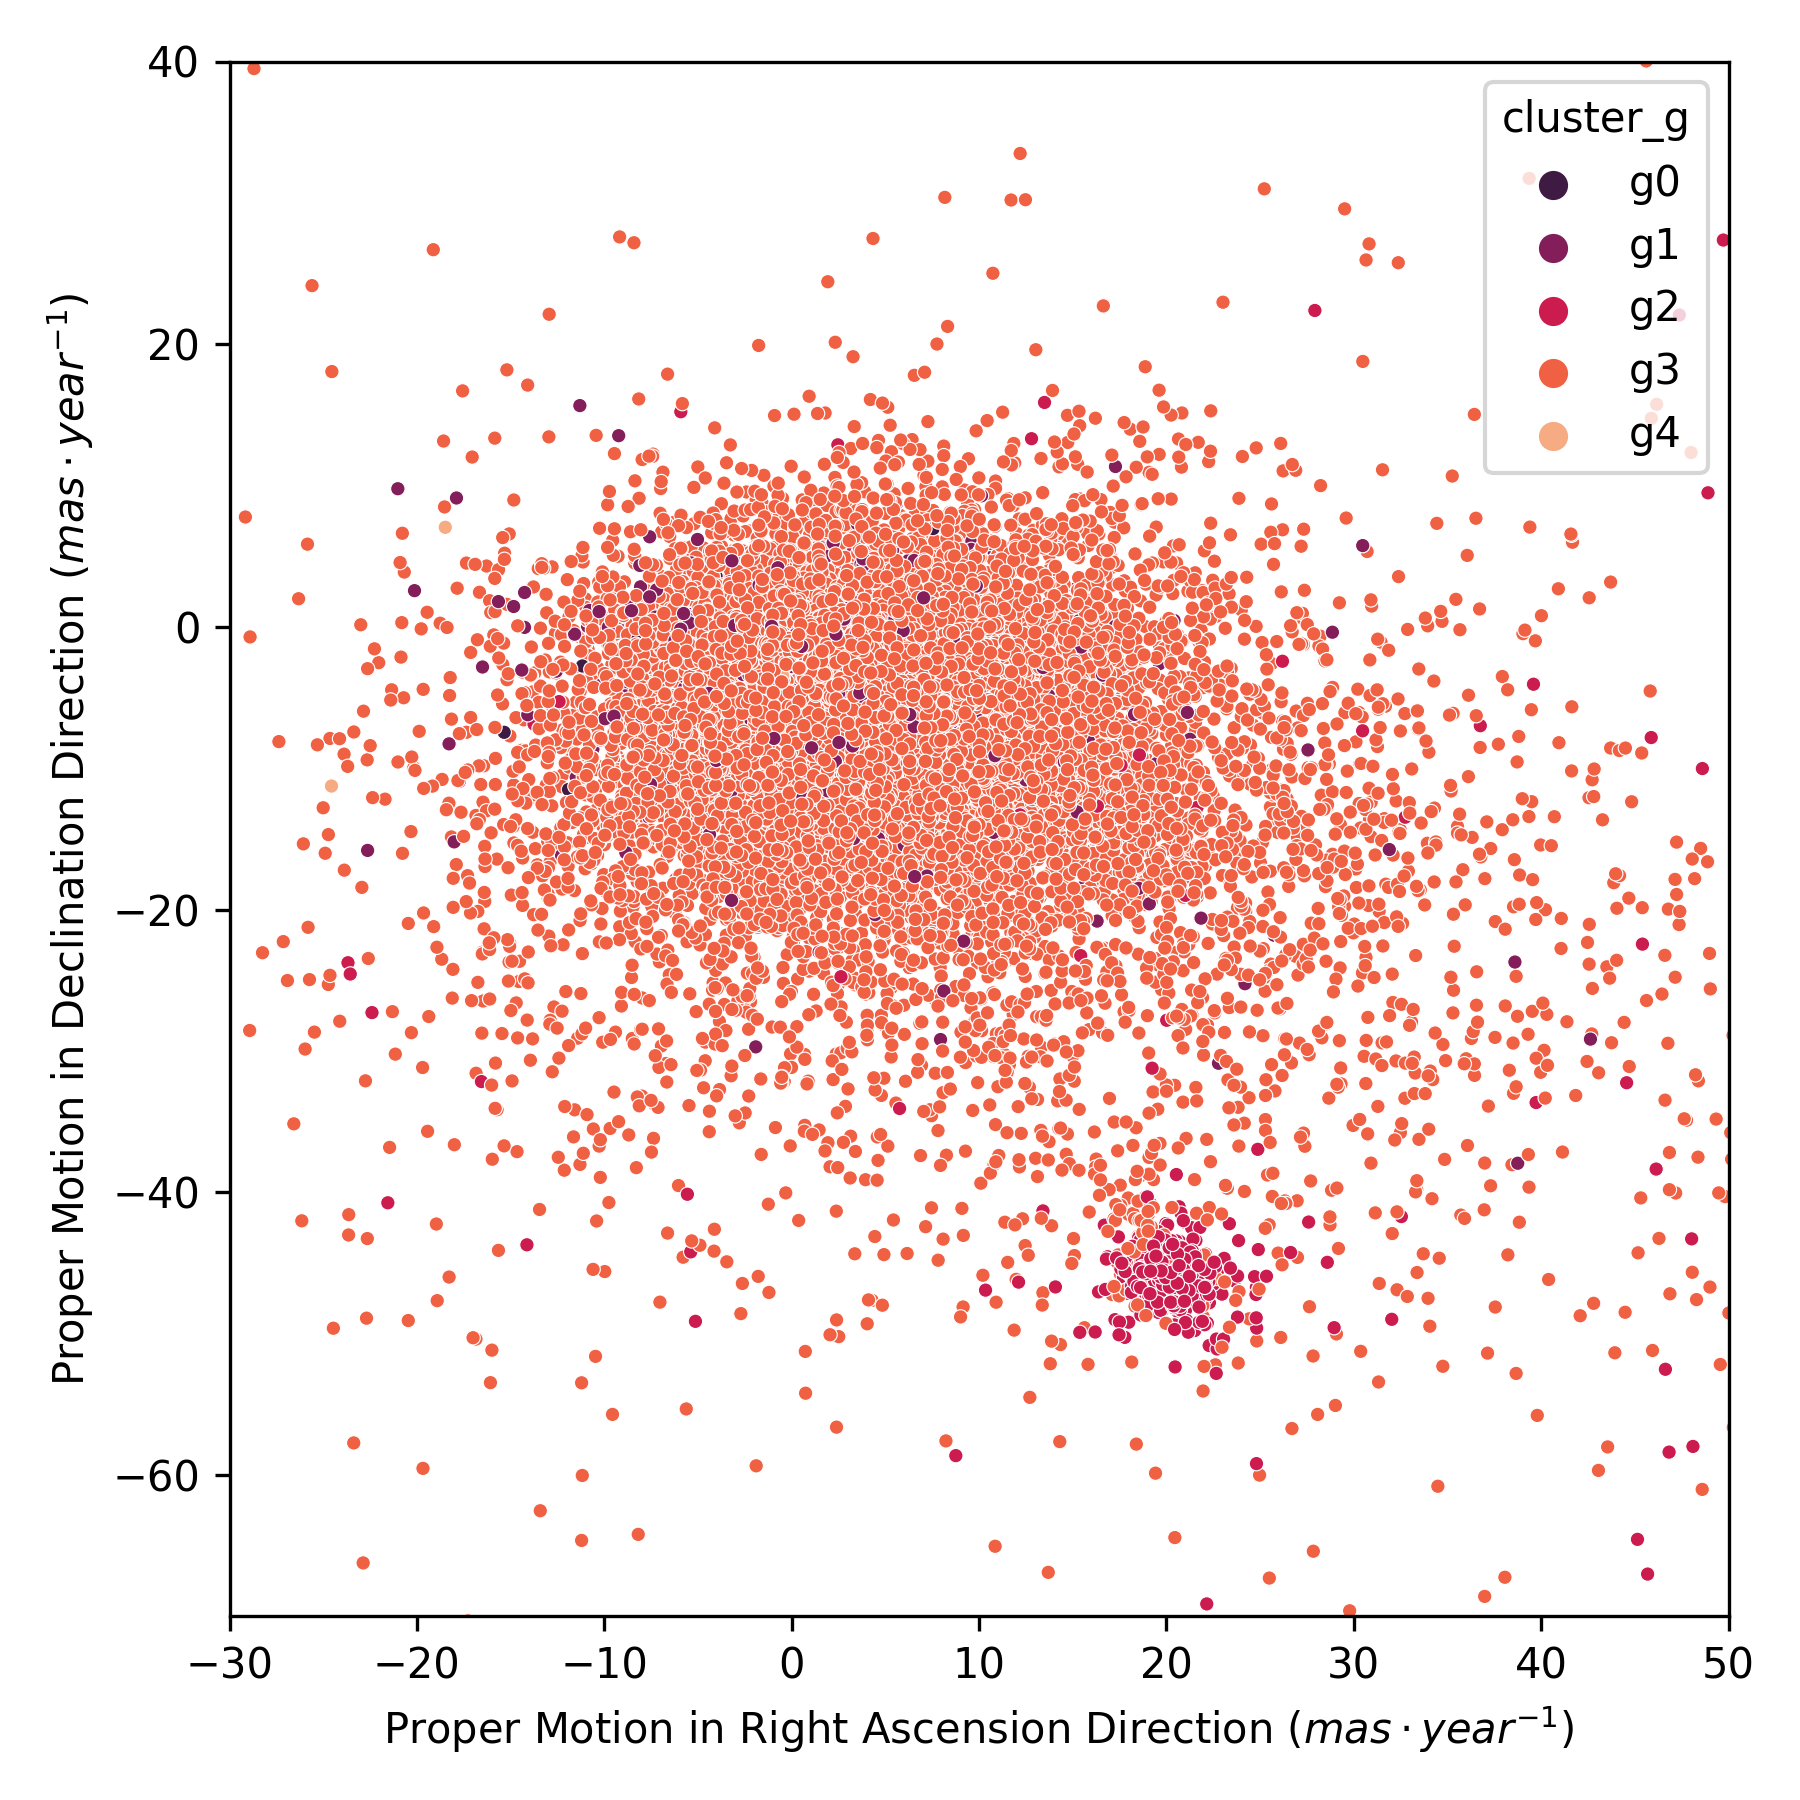
\includegraphics[width=\textwidth]{../figures/melotte_22/dec_pm_melotte_22.png}
      \caption{Proper Motion}
    \end{subfigure}
    \hfill
    \begin{subfigure}[t]{0.45\textwidth}
      \centering
      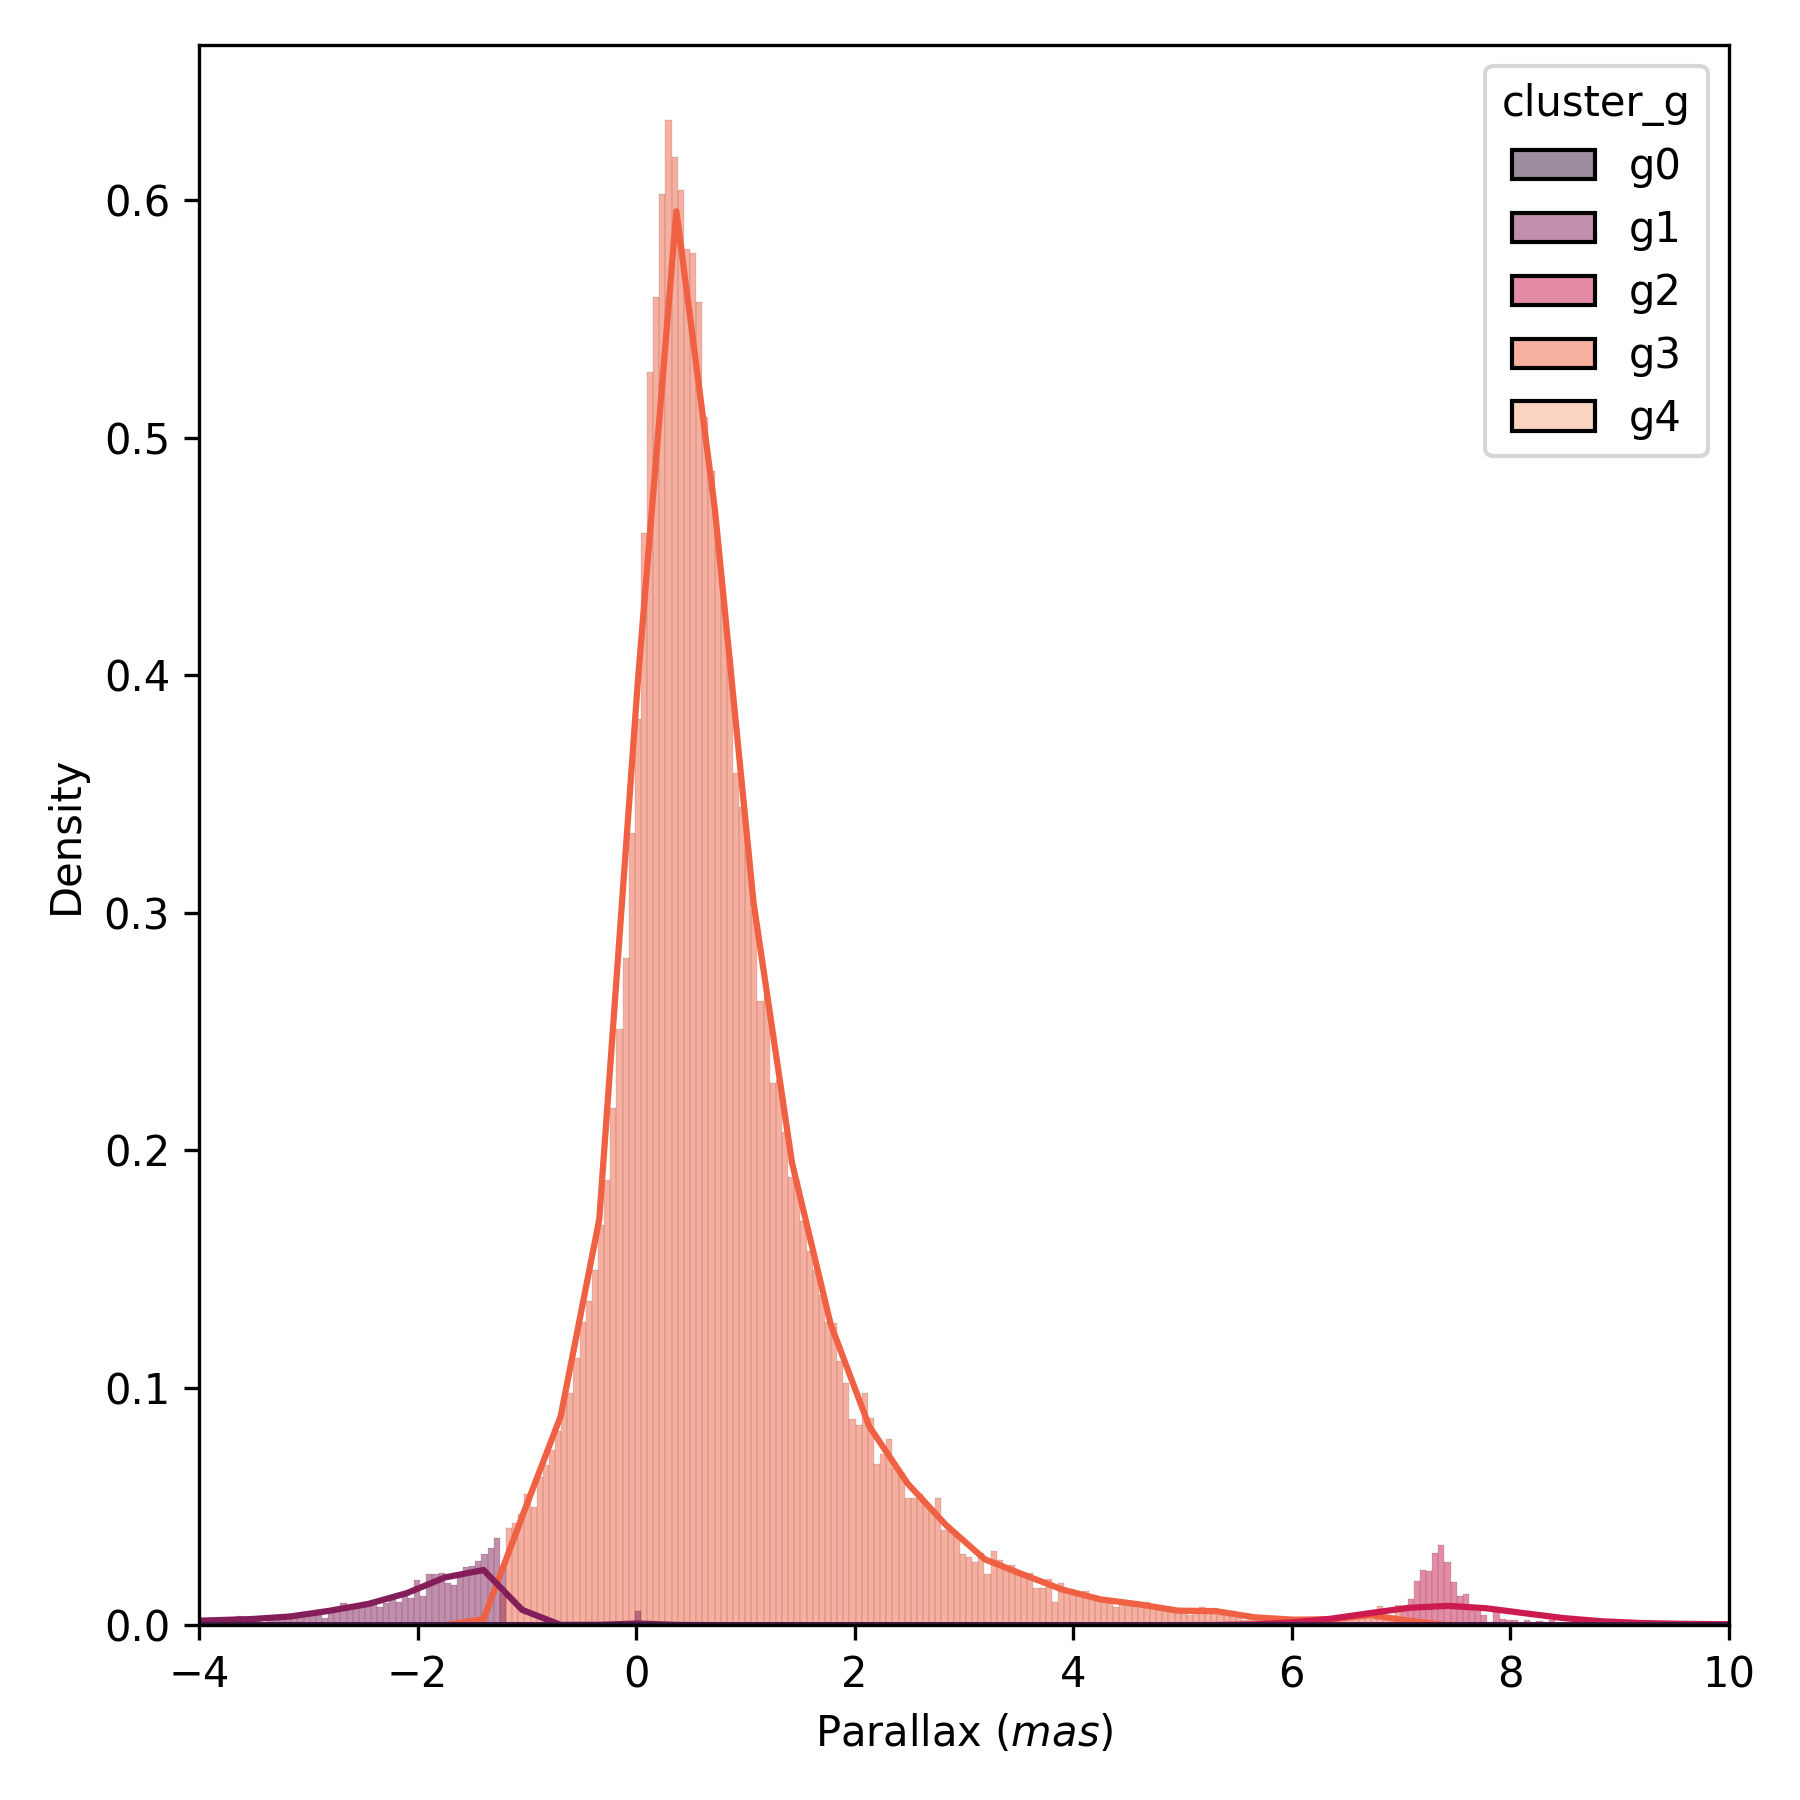
\includegraphics[width=\textwidth]{../figures/melotte_22/dec_parallax_melotte_22.png}
      \caption{Parallax}
    \end{subfigure}
  \end{subfigure}
  \caption{DEC model applied to Melotte 22}
  \label{fig:dec_melotte_22}
\end{figure}

The H-R diagram has been improved as well, and the isochrone curve of the open cluster is sharper than the one obtained with the K-Means algorithm
(Figure \ref{fig:kmeans_hr_diagram_melotte_22}).

\begin{figure}[htbp]
  \centering
  \begin{subfigure}{0.5\textwidth}
    \centering
    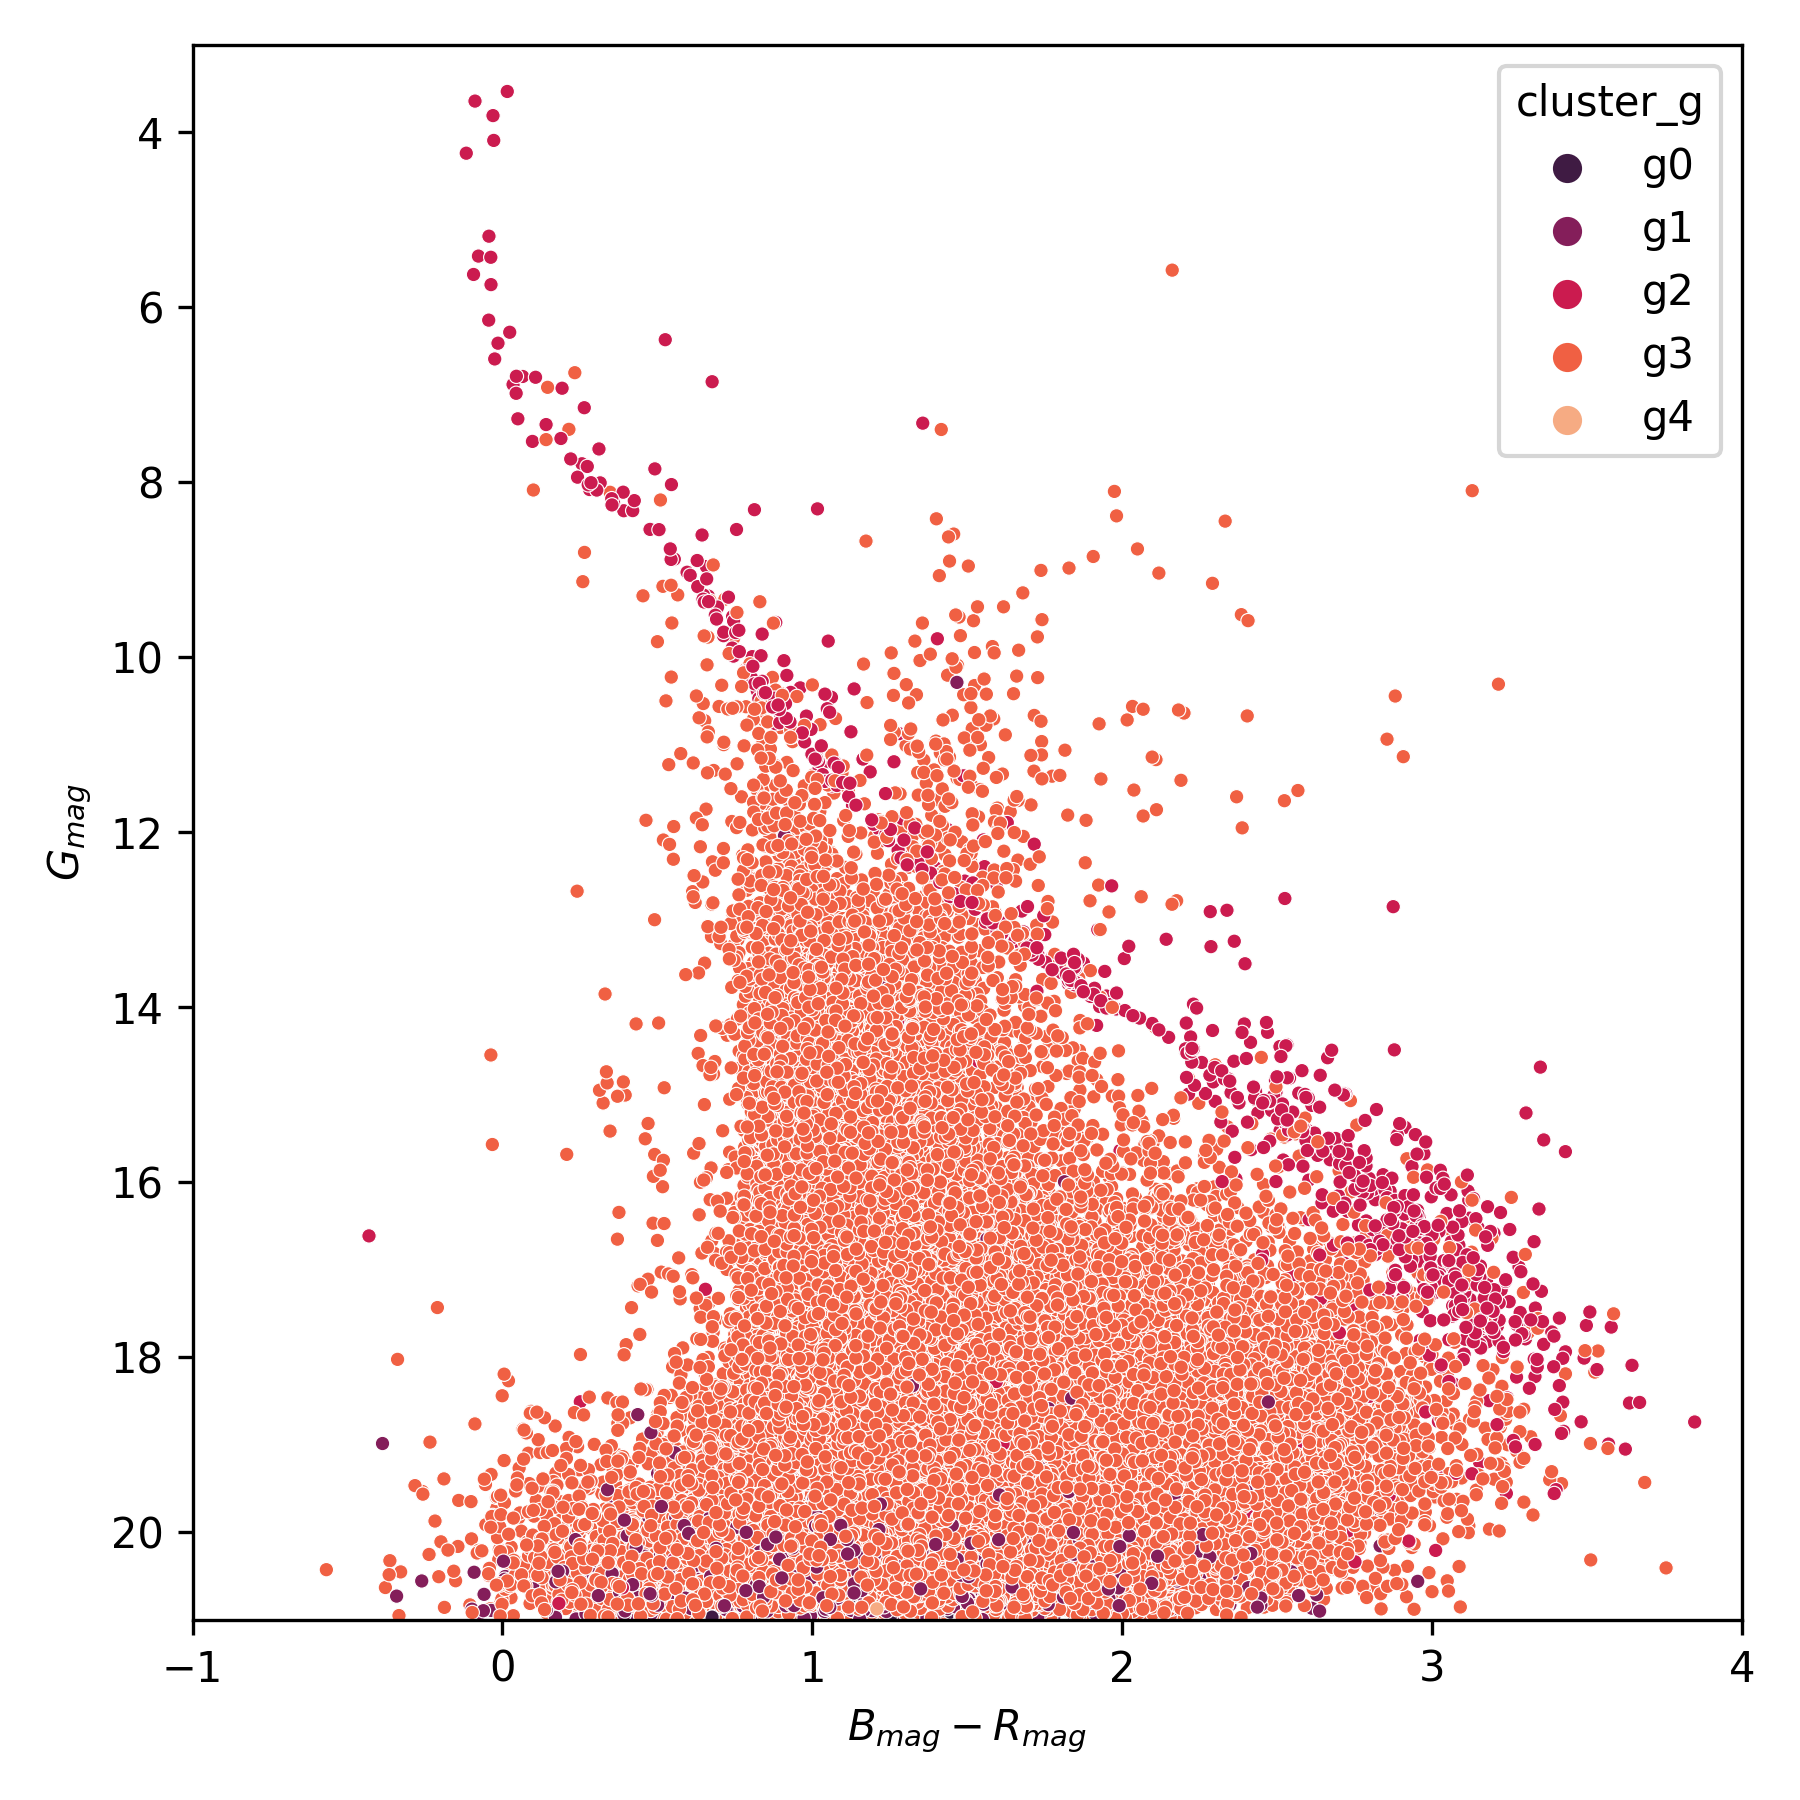
\includegraphics[width=\textwidth]{../figures/melotte_22/dec_hr_diagram_melotte_22.png}
  \end{subfigure}
  \caption{Melotte 22 H-R diagram with DEC characterization}
  \label{fig:dec_hr_diagram_melotte_22}
\end{figure}

\chapter{Results}

We have seen in the previous chapter that the DEC model is able to refine the clustering made by K-Means. This allows us to get
a more accurate characterization of the cluster.

In order to validate our model and be able to say how good or bad it is we need a different method to characterize the cluster
and compare one against each other.

For that reason we have used tools from the Virtual Observatory (VO) such as Clusterix and TOPCAT to characterize the studied clusters.

\section{Cluster Characterization with VO Tools}



\section{Comparison}

Until now, we have focus our study in Melotte 22 OC. Since our main aim is to get a model that fits well for a wide range of clusters,
we present now the results obtained for a selection of clusters with different topologies.

% TODO: Exposición de resultados y comentarios
% Es una exposición objetiva, sin valorar los resultados ni justificarlos.

\section{Discussion}

% Se aporta la discusión de los resultados presentados en el capítulo anterior. En este capítulo se puede discutir la relevancia de
% los resultados, presentar posibles explicaciones para los datos anómalos y resaltar aquellos datos que sean particularmente relevantes
% para el análisis del experimento.

\chapter{Conclusions and Future Work}

\section{Conclusions}

% Resumen final del trabajo y debe servir para informar del alcance y relevancia de la aportación.
% Suele estructurarse empezando con un resumen del problema tratado, de cómo se ha abordado y de por qué la solución sería válida.

% Es recomendable que incluya también un resumen de las contribuciones del trabajo, en el que se relacionen las contribuciones y los
% resultado obtenidos con ls objetivos planteados para el trabajo, discutiendo hasta qué punto has conseguido resolver los objetivos planteados.

\section{Further Research}

% Debería señalar las perspectivas de futuro que abre el trabajo desarrollado para el campo de estudio definido. En el fondo,
% debe justificar de qué modo puede emplearse la aportación desarrollada y en qué campos.

\listoffigures
\listoftables

\newpage

\bibliography{references}
\addcontentsline{toc}{chapter}{Bibliography}

\appendix
\chapter{Feature Selection}
\label{chap:feature_selection}

%\includepdf[pages=-]{anexo.pdf} # TODO: Descomentar cuando el artículo esté hecho
\end{document}
